%% One of these projects is the Alberta
%% Biodiversity Monitoring Initiative (ABMI) which every summer records
%% audio from over 1700 distinct locations from the entire area of the
%% province of Alberta and employs researchers to annotate the recordings
%% based on the precense of birds in order to monitor biodiversity
%% changes over time.  

%% In this work, I will describe my work in applying advanced audio
%% feature extraction, analysis and visualization tools to a variety of
%% different problem domains.  These domains include the study of Orca
%% vocalizations and the study of bird songs.  Although these application
%% areas are quite different, the tools and techniques that we use to
%% study each of them are very similar.

%% Self-Organized Maps, and Vector Quantization
%% are explored.


%% We will then examine the use of Self-Organized Maps (SOM) for
%% generating 2-dimensional representations of collections of audio that
%% are amenable for navigation by scientists.  SOMs are based an approach
%% similar to artifical neural networks, and we will examine the use of
%% artificial neural networks (ANN) to study audio.  In recent years, a
%% rexamination of the properties of real networks of neurons in living
%% systems has shown that these systems typically do not work with the
%% continuous, real valued model of traditional ANNs, but instead have
%% discrete signals that can be more accurately modelled as a sparse
%% representation.  Vector Quantization is a recent approach to the study
%% of sparse representations of audio, and we will examine the literature
%% of the use of this method, along with other methods that use a sparse
%% reprentation of audio.  We will finally provide a review of the
%% literature on recent developments in the tranformation of audio
%% features into a discrete form based on an alphabetic structure that
%% are amenable to analysis by tools from bioinformatics.  

%% The crosscorrelation of spectrogram images was explored in early work
%% by Clark \cite{clark87}.  In this work, songs of the swamp sparrow
%% were transformed into spectrograms, and a straightforward
%% cross-correlation of the spectrograms was used to get a quantitative
%% measure of their similarity.  They obtained good classification
%% results, from about 73\% for one song type to 92\% for another.

%% - Multi-pitch estimation of mixtures of signals \cite{klapuri08}
%% \cite{fujihara12}

%% - Automatic music transcription \cite{benetos12}

%% - Yin algorithm

%% The use of a Self-Organized Map for analyzing animal vocalizations
%% \cite{placer06} found that they could identify individual acoustic
%% elements in sounds, and allowed alarm calls to be classified with 91\%
%% accuracy.  They also mention that when the topological structure of
%% the SOM was transformed into a string representation, that different
%% digrams and trigrams were found to be associated with alarm calls for
%% different predators.  This paper is relevant to the current work in
%% that it shows one possible way that SOMs can be used to analyze audio,
%% and the framework described in this paper allows researchers to use a
%% SOM to analyze their own data.  It also provides another method for
%% turning audio data into a sequence of symbols, similar to the symbolic
%% approximation algorithms described in this thesis.


%% \subsection{Cochlear Models}

%% The models of the human auditory system developed by researchers
%% around the world have a fundamentally different approach in which
%% audio is filtered by a filterbank cascade that models features of the
%% human cochlea, the outputs of these filters are then processed by a
%% mechanism that is modeled on higher levels in the auditory periphery
%% that take this filterbank audio and generate two dimensional movie
%% frames that contain both frequency and an autocorrelation axis.  These
%% frames contain the fine timing information that is utilized by the
%% human hearing system to separate, localize and identify sounds.

%% Another type of audio feature extraction that is promising is features
%% based on models of the auditory cortex \cite{lyon82}.  These
%% algorithms model the properties of the cochlea and peripheral nervous
%% system\cite{lyon10}, and have at their core an adaptive filterbank
%% coupled to a triggered pulse model \cite{waltersphd}.  However, one
%% issue with these systems is that instead of a 1-dimensional (waveform)
%% or 2-dimensional (spectral), they lead to a 3-dimensional dataset in
%% which 2-D audio images change over time, which leads to a very large
%% amount of data.  Approaches using vector quantization could be used as
%% an input to our symbolic approximation algorithm in future work.

%% For my main project, I ported a new model of the human cochlea called
%% the Cascade of Asymmetric Filters and Resonators (CARFAC) \cite{lyon2011cas}  This model
%% is the latest in a series of ever more accurate and efficient models
%% of the human auditory system \cite{lyon82}.  Last summer I was
%% involved with investigating the performance of the Pole Zero Filter
%% Cascade (PZFC) model \cite{lyon10} in a variety of audio tasks, where
%% it performed very well.

%% - Correllogram

%% These algorithm 

%% - Dynamic Time Warping

%% Dynamic time warping (DTW) is a technique for measuring the similarity
%% of two sequence that many vary in time. It is mostly known in the context
%% of speech recognition \cite{sakoe78} but it has found applications in
%% many areas including video, motion and DNA sequence analysis. The use
%% of DTW to compute the similarity between two pulse rate contours in
%% the context of Orca calls has been explored in
%% \cite{brown07_orca_dtw}. In that work, a similarity matrix is
%% calculated containing all the DTW alignment costs between pairs of
%% pulse rate contours. This similarity matrix is then subsequently used
%% to calculate clusters which are then compared the ground truth call
%% labeling to assess the feasibility of call classification using this
%% approach.  

%% - Self-Organizing Maps

%% Self organizing maps have been used extensively in the visualization
%% of data for audio based music information retrieval \cite{cooper06}.
%% They have been used to analyze and organize music archives
%% \cite{rauber01a} \cite{rauber98a} \cite{rauber98b} \cite{rauber02a},
%% and to visualize the resulting music collections \cite{rauber03a}
%% \cite{pampalk04} \cite{rauber02}.  A particularily relvant study was
%% that of Palmalk in his paper Islands of Music \cite{pampalk03}.  SOMs
%% have also been used for audio retrieval, browing and constructivist
%% learning in several papers \cite{cano02} \cite{fruehwirth01}
%% \cite{honkela00}.  While the previous mentioned studies concentrated
%% on organizing whole classes of music, SOMs have also been applied to
%% smaller audio segments, including timbre \cite{toirvainen97},
%% energy-spectrum \cite{masugi04}, and musical time series analysis
%% \cite{capinteiro98}.

%% Self-organizing maps \cite{kohonen95a} are a multidimensional scaling
%% technique where a high dimension dataset is mapped to a lower,
%% typically 2-dimensional surface. SOMs and other such dimensionality
%% reduction tools allow users to visualize data relationships within
%% complex datasets.  There have been many applications of SOMs in Music
%% Information Retrieval including work by automatically analyzing and
%% organizing music archives \cite{rauber01a} \cite{rauber98b},
%% visualizing music genres \cite{pampalk03}\cite{pampalk03} and music
%% recommendation \cite{vembu05a}.  Self-organizing maps have been used
%% in Islands of Music \cite{RPM02} as well as the Databionic
%% visualization \cite{MUN05}.

%% - Vector Quantization

%% A paper highly relevant to our own, yet using very different
%% underlying audio features and Machine Learning algorithms is ``Sound
%% retrieval and ranking using sparse auditory representations''
%% \cite{lyon10} by Dick Lyon and his colleagues at Google.  In this
%% paper, the authors describe a system designed to help them to create
%% systems to understand sounds, and they use both a novel audio feature
%% representation based on models of human hearing combined with a novel
%% Machine Learning algorithm previously used for image retrieval named
%% PAMIR (Passive Aggressive Model for Image Retrieval).  In this system,
%% the data was represented as sparse vectors, which is quite different
%% from the dense feature vectors commonly used in DSP.  Sparse vectors
%% have mostly zero values, with just a few non-zero values, and dense
%% vectors have numbers in almost all their elements.  Sparse vectors are
%% commonly found in Machine Learning systems that work with text.

%% In their system, they compare the results of the typical features that
%% are used in Machine Hearing, the Mel-Frequency Cepstral Coefficients
%% \cite{Logan00melfrequency} (MFCC) with those of their novel algorithm,
%% one based on models of the human peripheral auditory system which used
%% a filterbank called the Pole-Zero Filterbank Cascade (PZFC) and used
%% this data to make a series of Stabilized Auditory Images (SAIs).
%% While on one hand the MFCC system outputs a one dimensional vector for
%% each time slice, producing an image for the sound file when these time
%% slices are stacked, the SAI system on the other hand generates a two
%% dimensional vector at each time slice, which can be represented as an
%% image which can be stacked to form a movie.  The authors describe a
%% system whereby these images are divided into a number of regions, and
%% the section of the images that are in these regions are then clustered
%% based on their similarity using vector quantization to generate a
%% dictionary using an training set of audio.  This dictionary is then
%% used to do vector quantization of test audio, and these features are
%% used as input to the PAMIR system.

%% PAMIR is a new algorithm for doing mappings from a huge sparse feature
%% set to a very large query-term set, and was traditionally used in
%% image recognition \cite{chechik10} to generate tags for images on
%% Google Image search.  In this context, PAMIR is used to tag SAI images
%% in order to add tag annotations to sound files.  The authors show
%% impressive results, with an average precision of 35\% and best
%% precision at top-1 of 73\%.

%% This paper is directly relevant to my current paper, and in fact there
%% are a number of the algorithms in this paper that we want to implement
%% in my own OpenMIR system.  However, it should be noted that while
%% these algorithms, specifically the modeling of the auditory cortex and
%% the SAI model, do show a substantial increase in performance over
%% traditional techniques, they do come with a substantial performance
%% hit, and are typically much slower than traditional algorithms since
%% they often must do an $O(n^2)$ step to calculate the SAI image while
%% traditional FFT techniques only must do an $O(n(log(n)))$ step.  In
%% any case, the method of using vector quantization, SAI images and
%% advanced Machine Learning techniques such as PAMIR shows great promise
%% in the future in my work.

%% A paper highly relevant to our own, yet using very different
%% underlying audio features and Machine Learning algorithms is ``Sound
%% retrieval and ranking using sparse auditory representations''
%% \cite{lyon10} by Dick Lyon and his colleagues at Google.  In this
%% paper, the authors describe a system designed to help them to create
%% systems to understand sounds, and they use both a novel audio feature
%% representation based on models of human hearing combined with a novel
%% Machine Learning algorithm previously used for image retrieval named
%% PAMIR (Passive Aggressive Model for Image Retrieval).  In this system,
%% the data was represented as sparse vectors, which is quite different
%% from the dense feature vectors commonly used in DSP.  Sparse vectors
%% have mostly zero values, with just a few non-zero values, and dense
%% vectors have numbers in almost all their elements.  Sparse vectors are
%% commonly found in Machine Learning systems that work with text.

%% In their system, they compare the results of the typical features that
%% are used in Machine Hearing, the Mel-Frequency Cepstral Coefficients
%% \cite{Logan00melfrequency} (MFCC) with those of their novel algorithm,
%% one based on models of the human peripheral auditory system which used
%% a filterbank called the Pole-Zero Filterbank Cascade (PZFC) and used
%% this data to make a series of Stabilized Auditory Images (SAIs).
%% While on one hand the MFCC system outputs a one dimensional vector for
%% each time slice, producing an image for the sound file when these time
%% slices are stacked, the SAI system on the other hand generates a two
%% dimensional vector at each time slice, which can be represented as an
%% image which can be stacked to form a movie.  The authors describe a
%% system whereby these images are divided into a number of regions, and
%% the section of the images that are in these regions are then clustered
%% based on their similarity using vector quantization to generate a
%% dictionary using an training set of audio.  This dictionary is then
%% used to do vector quantization of test audio, and these features are
%% used as input to the PAMIR system.

%% \section{Auditory Sparse Coding}

%% The concept of sparsity has attracted considerable interest in the
%% field of machine learning in the past few years.  Sparse feature
%% vectors contain mostly values of zero and one or a few non-zero
%% values.  Although these feature vectors can be classified by
%% traditional machine learning algorithms, such as SVM, there are various
%% recently-developed algorithms that explicitly take advantage of
%% the sparse nature of the data, leading to massive speedups in time, as
%% well as improved performance.  Some fields that have benefited from
%% the use of sparse algorithms are finance, bioinformatics, text mining
%% \cite{balakrishnan2008}, and image classification \cite{chechik2010}.
%% Because of their speed, these algorithms perform well on very large
%% collections of data \cite{bottou2007}; large collections are becoming 
%% increasingly relevant given the huge amounts of data collected and warehoused 
%% by Internet businesses.

%% This fine-timing information from the cochlea can be made use of in
%% later stages of processing to yield a three-dimensional representation
%% of audio, the stabilized auditory image (SAI)\cite{patterson2000},
%% which is a movie-like representation of sound which has a dimension of
%% `time-interval' in addition to the standard dimensions of time and
%% frequency in the spectrogram. The periodicity of the waveform gives
%% rise to a vertical banding structure in this time interval dimension,
%% which provides information about the sound which is complementary to
%% that available in the frequency dimension.

%% There is also growing evidence that in the human nervous
%% system sensory inputs are coded in a sparse manner; that is, only
%% small numbers of neurons are active at a given time
%% \cite{olshausen2004}.  Therefore, when modeling the human auditory
%% system, it may be advantageous to investigate this property of
%% sparseness in relation to the mappings that are being developed. The
%% nervous systems of animals have evolved over millions of years to be
%% highly efficient in terms of energy consumption and computation. 
%% Looking into the way sound signals are handled by the auditory
%% system could give us insights into how to make our algorithms more
%% efficient and better model the human auditory system.

%% One advantage of using sparse vectors is that such coding allows very fast
%% computation of similarity, with a trainable similarity measure 
%% \cite{chechik2010}. The efficiency results from storing, accessing, and doing 
%% arithmetic operations on only the non-zero elements of the vectors.   
%% In one study that examined the performance of sparse
%% representations in the field of natural language processing, a 20- to
%% 80-fold speedup over LIBSVM was found \cite{haffner2006}.  They
%% comment that kernel-based methods, like SVM, scale quadratically with
%% the number of training examples and discuss how sparsity can allow
%% algorithms to scale linearly based on the number of training examples.

%% In the paper ``Monitoring and Mining Insect Sounds in Visual
%% Space''\cite{hao12}, Hao et al. describe a novel method for data
%% mining large databases of insect sounds. 

%% Campana-Keogh (CK) measure \cite{campana2010} which uses the
%% concept that two images are similar if one image can be used to
%% compress the other image. 

%% \section{Bioinformatics}

%% The transcription of time series data into a character sequence that
%% can be consumed by bioinformatics sequence alignment tools is a
%% nontrivial task.  An attempt towards this goal is Symbolic Aggregate
%% Approximation (SAX) which was proposed by Lin et al. in
%% \cite{Lin2003}. The underlying idea of SAX is to parse a time series
%% using a sliding window and to generate a character sequence that
%% approximates the signal's normalized slope using a technique called
%% Piecewise Aggregate Approximation (PAA).  SAX is most useful in cases
%% where the data is not on an absolute scale.  

%% For the Machine Learning half of the project, a variety of Machine
%% Learning systems and algorithms were used and comparison of them in is
%% provided in the evaluation section.  Results have been produced for a
%% Logistic Regression system using a Stochastic Gradient Descent
%% algorithm on Mahout, a distributed Machine Learning system implemented
%% as a Java library on top of Hadoop, an open source clone of the Google
%% File System (GFS) and Google MapReduce system.  These results are
%% compared to a Logistic Regression system using a quasi Newton solver
%% as implemented in Weka, a popular system for Machine Learning and show
%% timing and classification results of this system run as a grid style
%% parallel job on Westgrid.  These results for Logistic Regression are
%% then compared to three different implementations of a Support Vector
%% Machine (SVM) classifier.  The first of these is simply the SVM mode
%% in Weka but run in a grid-style distributed manner.  The second of
%% these is a parallel version of the SVM algorithm, PSVM
%% \cite{chang07psvm}.  The third of these is a hybrid audio feature
%% extraction and SVM developed in the Marsyas framework.  These three
%% different systems will be compared and contrasted in the Evaluation
%% section.

%% In this project we will use the Mahout Machine Learning framework on
%% top of a Hadoop installation to process the audio feature vectors
%% output by Marsyas and to gain insights into the vocalization data in
%% the Orchive. 

%% Mahout is a Machine Learning framework that interacts closely with
%% Hadoop to both store the data and also run the Machine Learning
%% algorithms.  Hadoop is an open source port of the GFS
%% \cite{ghemawat03} and MapReduce \cite{dean08} infrastructure and
%% allows users to run large jobs that follow the map reduce paradigm.
%% In this scheme, a parallel job is split into two phases, a map phase
%% and a reduce phase.  In the map phase, key value pairs are generated
%% by some given algorithm from an input file, this same process occurs
%% in parallel on many other nodes, and the data that is used by a given
%% map is determined by the locality of data on that node.  These key
%% value pairs are then sorted and shuffled to a set of reduce nodes,
%% which take the collections of key value pairs and do an operation on
%% them that in some way combines, or reduces, the data.  These map and
%% reduce functions can be thought of as similar to the map and reduce
%% functions in functional programming, however, it should be noted that
%% this is a loose similarity due to the lack of higher order functions
%% in the current MapReduce implementation.  Many algorithms have been
%% ported to use this MapReduce type system, some of the most natural are
%% those that process large collections of text for building inverted
%% indexes or other tasks for searches, which is not surprising noting
%% the provenance of the MapReduce algorithm.  For other tasks, such as
%% those common in audio feature extraction, the reduce phase is simply
%% an identity reduce, where the map outputs are copied verbatim to the
%% reduce outputs.  It is easier and more natural to make some algorithms
%% more efficient in a MapReduce context than others.

%% The Mahout Machine Learning framework has implemented many different
%% Machine Learning algorithms in it's framework, including clustering,
%% recommendation and classification algorithms.  In our current work we
%% are more interested in classification than either recommendation or
%% clustering, and Mahout boasts support for the following classification
%% algorithms: Logistic Regression (SGD), Bayesian, Support Vector
%% Machines (SVM), Perceptron and Winnow, Neural Network, Random Forests,
%% Restricted Boltzmann Machines, Online Passive Aggressive, Boosting and
%% Hidden Markov Models.  However, after investigation, it appears most
%% of these algorithms are in a definite alpha state, and require
%% patching of the main source tree with external files.  The two most
%% well supported classification algorithms in Mahout are the Logistic
%% Regression classifier, using a Stochastic Gradient Descent (SGD)
%% engine, and a Naive Bayesian classifier.  Upon extensive
%% investigation, the Bayesian classifier makes many internal assumptions
%% of the input being of large bodies of written text and was not
%% suitable for our use case.  However, the Logistic Regression
%% classifier was well suited to our data and performed well in our
%% tests.

%% One advantage of using the Mahout Machine Learning framework was that
%% it stored its input and output data on HDFS, the Hadoop Distributed
%% Filesystem.  When working with the huge amounts of data that are
%% generated by audio feature extraction and Machine Learning
%% experiments, managing and transferring experimental results from the
%% grid servers to the production web servers is often a time consuming
%% and error prone procedure.  After our experience with Hadoop, we have
%% integrated it into web application and use the WebHDFS system to serve
%% all experimental results to users.  These users interact with a web
%% application that displays some data obtained from the production web
%% server but also displays the results of experiments as data served
%% live from a WebHDFS system that is being populated by the experimental
%% results from live requests from scientists.

%% - Side Band Intervals


%% - Stabilized Auditory Image


%% \section{Auditory Sparse Coding}

%% The concept of sparsity has attracted considerable interest in the
%% field of machine learning in the past few years.  Sparse feature
%% vectors contain mostly values of zero and one or a few non-zero
%% values.  Although these feature vectors can be classified by
%% traditional machine learning algorithms, such as SVM, there are
%% various recently-developed algorithms that explicitly take advantage
%% of the sparse nature of the data, leading to massive speedups in time,
%% as well as improved performance.  Some fields that have benefited from
%% the use of sparse algorithms are finance, bioinformatics, text mining
%% \cite{balakrishnan2008}, and image classification \cite{chechik2010}.
%% Because of their speed, these algorithms perform well on very large
%% collections of data \cite{bottou2007}; large collections are becoming
%% increasingly relevant given the huge amounts of data collected and
%% warehoused by Internet businesses.

%% In this chapter, we discuss the application of sparse feature vectors
%% in the field of audio analysis, and specifically their use in conjunction with 
%% preprocessing systems that model the human auditory system. We present early
%% results that demonstrate the applicability of the combination of 
%% auditory-based processing and sparse coding to content-based audio analysis 
%% tasks.

%% Traditional approaches to audio analysis problems typically employ a 
%% short-window fast Fourier transform (FFT) as the first stage of the processing 
%% pipeline. In such systems a short, perhaps 25ms, segment of audio is taken 
%% from the input signal and windowed in some way, then the FFT of that segment 
%% is taken. The window is then shifted a little, by perhaps 10ms, and the 
%% process is repeated. This technique yields a two-dimensional spectrogram of 
%% the original audio, with the frequency axis of the FFT as one dimension, and 
%% time (quantized by the step-size of the window) as the other dimension.

%% While the spectrogram is easy to compute, and a standard engineering
%% tool, it bears little resemblance to the early stages of the
%% processing pipeline in the human auditory system. The mammalian
%% cochlea can be viewed as a bank of tuned filters the output of which
%% is a set of band-pass filtered versions of the input signal that are
%% continuous in time. Because of this property, fine-timing information
%% is preserved in the output of cochlea, whereas in the spectrogram
%% described above, there is no fine-timing information available below
%% the 10ms hop-size of the windowing function.

%% This fine-timing information from the cochlea can be made use of in
%% later stages of processing to yield a three-dimensional representation
%% of audio, the stabilized auditory image (SAI)\cite{patterson2000},
%% which is a movie-like representation of sound which has a dimension of
%% `time-interval' in addition to the standard dimensions of time and
%% frequency in the spectrogram. The periodicity of the waveform gives
%% rise to a vertical banding structure in this time interval dimension,
%% which provides information about the sound which is complementary to
%% that available in the frequency dimension. A single example frame of a
%% stabilized auditory image is shown in Figure~\ref{fig:sai}.

%% While we believe that such a representation should be useful for audio
%% analysis tasks, it does come at a cost. The data rate of the SAI is
%% many times that of the original input audio, and as such some form of
%% dimensionality reduction is required in order to create features at a
%% suitable data rate for use in a recognition system. One approach to
%% this problem is to move from a the dense representation of the SAI to
%% a sparse representation, in which the overall dimensionality of the
%% features is high, but only a limit number of the dimensions are
%% nonzero at any time.

%% In recent years, machine learning algorithms that utilize the
%% properties of sparsity have begun to attract more attention and have
%% been shown to outperform approaches that use dense feature vectors.
%% One such algorithm is the passive-aggressive model for image retrieval
%% (PAMIR), a machine learning algorithm that learns a ranking function
%% from the input data, that is, it takes an input set of documents and
%% orders them based on their relevance to a query. PAMIR was originally
%% developed as a machine vision method and has demonstrated excellent
%% results in this field.

%% There is also growing evidence that in the human nervous system
%% sensory inputs are coded in a sparse manner; that is, only small
%% numbers of neurons are active at a given time \cite{olshausen2004}.
%% Therefore, when modeling the human auditory system, it may be
%% advantageous to investigate this property of sparseness in relation to
%% the mappings that are being developed. The nervous systems of animals
%% have evolved over millions of years to be highly efficient in terms of
%% energy consumption and computation.  Looking into the way sound
%% signals are handled by the auditory system could give us insights into
%% how to make our algorithms more efficient and better model the human
%% auditory system.

%% One advantage of using sparse vectors is that such coding allows very
%% fast computation of similarity, with a trainable similarity measure
%% \cite{chechik2010}. The efficiency results from storing, accessing,
%% and doing arithmetic operations on only the non-zero elements of the
%% vectors.  In one study that examined the performance of sparse
%% representations in the field of natural language processing, a 20- to
%% 80-fold speedup over LIBSVM was found \cite{haffner2006}.  They
%% comment that kernel-based methods, like SVM, scale quadratically with
%% the number of training examples and discuss how sparsity can allow
%% algorithms to scale linearly based on the number of training examples.

%% In this chapter, we use the stabilized auditory image (SAI) as the
%% basis of a sparse feature representation which is then tested in a
%% sound ranking task and a music information retrieval task. In the
%% sound raking task, we generate a two-dimensional SAI for each time
%% slice, and then sparse-code those images as input to PAMIR.  We use
%% the ability of PAMIR to learn representations of sparse data in order
%% to learn a model which maps text terms to audio features.  This PAMIR
%% model can then be used rank a list of unlabeled sound effects
%% according to their relevance to some text query. We present results
%% that show that in certain tasks our methods can outperform highly
%% tuned FFT based approaches. We also use similar sparse-coded SAI
%% features as input to a music genre classification system. This system
%% uses an SVM classifier on the sparse features, and learns text terms
%% associated with music. The system was entered into the annual music
%% information retrieval evaluation exchange evaluation (MIREX 2010).

%% Results from the sound-effects ranking task show that sparse
%% auditory-model-based features outperform standard MFCC features,
%% reaching precision about 73\% for the top-ranked sound, compared to
%% about 60\% for standard MFCC and 67\% for the best MFCC variant.
%% These experiments involved ranking sounds in response to text queries
%% through a scalable online machine learning approach to ranking.

%% In our system we have taken inspiration from the human auditory system
%% in order to come up with a rich set of audio features that are
%% intended to more closely model the audio features that we use to
%% listen and process music.  

%% Such fine timing relations are discarded by traditional spectral
%% techniques.  A motivation for using auditory models is that the
%% auditory system is very effective at identifying many sounds.  This
%% capability may be partially attributed to acoustic features that are
%% extracted at the early stages of auditory processing.  We feel that
%% there is a need to develop a representation of sounds that captures
%% the full range of auditory features that humans and animals use to
%% discriminate and identify different sounds, so that machines have a
%% chance to do so as well.

%% This SAI representation generates a 2D image from each section of
%% waveform from an audio file.  We then reduce each image in several
%% steps: first cutting the image into overlapping boxes converted to
%% fixed resolution per box; second, finding row and column sums of these
%% boxes and concatenating those into a vector; and finally vector
%% quantizing the resulting medium-dimensionality vector, using a
%% separate codebook for each box position.  The VQ codeword index is a
%% representation of a 1-of-N sparse code for each box, and the
%% concatenation of all of those sparse vectors, for all the box
%% positions, makes the sparse code for the SAI image.  The resulting
%% sparse code is accumulated across the audio file, and this histogram
%% (count of number of occurrences of each codeword) is then used as
%% input to an SVM \cite{yh05} classifier\cite{chapelle2006}.  This
%% approach is similar to that of the ``bag of words'' concept,
%% originally from natural language processing, but used heavily in
%% computer vision applications as ``bag of visual words''; here we have
%% a ``bag of auditory words'', each ``word'' being an abstract feature
%% corresponding to a VQ codeword.  The bag representation is a list of
%% occurrence counts, usually sparse.


%% \section{Algorithm}

%% In our experiments, we generate a stream of SAIs using a series of modules
%% that process an incoming audio stream through the various stages of the 
%% auditory model. The first module filters the audio using the
%% pole--zero filter cascade (PZFC) \cite{lyon10}, then subsequent modules find 
%% strobe points in this audio, and generate a stream of SAIs at a rate of 50 per 
%% second. The SAIs are then cut into boxes and are transformed into a high 
%% dimensional dense feature vector \cite{rehn2009} which is vector quantized to 
%% give a high dimensional sparse feature vector. This sparse vector is then used 
%% as input to a machine learning system which performs either ranking or 
%% classification. This whole process is shown in diagrammatic form in Figure 
%% ~\ref{fig:flowchart}

%% We first process the audio with the pole--zero filter cascade (PZFC)
%% \cite{lyon10}, a model inspired by the dynamics of the human
%% cochlea. The PZFC is a cascade of a large number of simple filters
%% with an output tap after each stage. The effect of this filter cascade
%% is to transform an incoming audio signal into a set of band-pass
%% filtered versions of the signal. In our case we used a cascade with 95
%% stages, leading to 95 output channels. Each output channel is
%% half-wave rectified to simulate the output of the inner hair cells
%% along the length of the cochlea. The PZFC also includes an automatic
%% gain control (AGC) system that mimics the effect of the dynamic
%% compression mechanisms seen in the cochlea. A smoothing network, fed
%% from the output of each channel, dynamically modifies the
%% characteristics of the individual filter stages. The AGC can respond
%% to changes in the output on the timescale of milliseconds, leading to
%% very fast-acting compression. One way of viewing this filter cascade
%% is that its outputs are an approximation of the instantaneous neuronal
%% firing rate as a function of cochlear place, modeling both the
%% frequency filtering and the automatic gain control characteristics of
%% the human cochlea \cite{lyon1990}. The PZFC parameters used for the
%% sound-effects ranking task are described in \cite{lyon10}. We did not
%% do any further tuning of this system to the problems of genre, mood or
%% song classification; this would be a fruitful area of further
%% research.

%% \subsection{Image Stabilization}

%% The output of the PZFC filterbank is then subjected to a process of
%% strobe finding where large peaks in the PZFC signal are found.  The
%% temporal locations of these peaks are then used to initiate a process
%% of temporal integration whereby the stabilized auditory image is
%% generated.  These strobe points ``stabilize'' the signal in a manner
%% analogous to the trigger mechanism in an oscilloscope.  When these
%% strobe points are found, a modified form of autocorrelation, known as
%% strobed temporal integration, which is like a sparse version of
%% autocorrelation where only the strobe points are correlated against
%% the signal. Strobed temporal integration has the advantage of being
%% considerably less computationally expensive than full autocorrelation.

%% \subsection{Box Cutting}

%% We then divide each image into a number of overlapping boxes using the
%% same process described in \cite{lyon10}.  We start with rectangles of
%% size 16 lags by 32 frequency channels, and cover the SAI with these
%% rectangles, with overlap.  Each of these rectangles is added to the
%% set of rectangles to be used for vector quantization.  We then
%% successively double the height of the rectangle up to the largest size
%% that fits in an SAI frame, but always reducing the contents of each
%% box back to 16 by 32 values.  Each of these doublings is added to the
%% set of rectangles.  We then double the width of each rectangle up to
%% the width of the SAI frame and add these rectangles to the SAI frame.
%% The output of this step is a set of 44 overlapping rectangles. The
%% process of box-cutting is shown in Figure ~\ref{fig:boxcutting}. In
%% order to reduce the dimensionality of these rectangles, we then take
%% their row and column marginals and join them together into a single
%% vector.

%% The resulting dense vectors from all the boxes of a frame are then
%% converted to a sparse representation by vector quantization.

%% \subsection{Campana}

%% In the paper ``Monitoring and Mining Insect Sounds in Visual
%% Space''\cite{hao12}, Hao et al. describe a novel method for data
%% mining large databases of insect sounds.  Their method is completely
%% automated, and does not require human experts to label data, as is the
%% case in most other systems of this type.  They perform classification
%% of sounds based on the spectrogram, a visual representation of a sound
%% that gives a frequency versus time plot of a sound.  They use a recent
%% distance measure called the Campana-Keogh (CK) measure to compare the
%% textures of two images.

%% The paper first describes the importance of monitoring and measuring
%% of the sounds of animals and insects.  In the natural habitat, the
%% sounds of animals can be used to determine how many animals are in a
%% location and what species these animals are, and can help scientists
%% measure the biodiversity of a location, and how this biodiversity
%% changes over time.  There is recent interest in this field of study
%% \cite{wimmer2010} \cite{seuer2008} as a method for determining the
%% biodiversity changes in regions over time.  The authors then say that
%% an automated system for detecting insects would also be useful from a
%% commercial point of view,

%% The paper then goes on to say that in laboratory settings, it would
%% also be advantageous to have an automated system that could segment
%% and classify recordings.  Currently this task often requires
%% researchers to annotate hundreds of recordings by hand, which is a
%% very time intensive task.  As a scientist who has done many hours of
%% hand annotating of large sound archives, I can attest to the
%% difficulty and time-consuming nature of this task.

%% The authors then say that there are many problems with current methods
%% of detecting, segmenting and classifying the sounds and vocalizations
%% of animals.  Current methods require researchers to manually annotate
%% recordings and to generate a large corpus of data to be used by
%% classification algorithms.  These algorithms often have a large number
%% of tunable parameters, some of which can be automatically determined
%% from the large amount of training data, and some which have to be
%% manually explored by the researchers.  In addition, many of these
%% algorithms are computationally expensive and cannot be deployed in the
%% field.  I have found these facts to be true in my own research, and I
%% appreciate the fact that the authors spend time discussing the
%% problems faced by researchers studying bioacoustics.

%% In this section, they first define a sound sequence as a continuous
%% sequence of real valued data.  They then go on to define a spectrogram
%% as a visual spectral representation of an acoustic signal.  They
%% define a sliding window as a local subsection of a sound sequence, and
%% define a subsequence and a way to measure distances between
%% subsequences.

%% They then move on to more interesting definitions, first of the
%% entropy of a sound sequence dataset:
%% 	\[ E(D) = -p(X)log(p(X)) - p(Y)log(p(Y)) \]

%% The information gain for a given splitting strategy is then defined as
%% 	\[ Gain = E(D) - E'(D) \]

%% Where $E(D)$ and $E'(D)$ are the entropy before and after $D$ is
%% partitioned into $D_1$ and $D_2$.

%% 	\[ E(D) = f(D_1)E(D_1) + f(D_2)E(D_2) \] 

%% Where $f(D_1)$ and $f(D_2)$ are the fraction of the objects that are
%% in $D_1$ and $D_2$, respectively.

%% They then point out that given a linear ordering of annotated objects
%% in $D$, there exist at most $|D|-1$ distinct splitting points that
%% divide the ordered objects into two distinct sets.  Finally, they
%% define a sound fingerprint for a species as the subsequence from P
%% along with its best splitting point that produces the largest
%% information gain when compared with the non-matching sequences U.

%% They then go on to provide an figure that explains in rough detail
%% what their distance measure looks like.  This is shown here in Figure
%% \ref{fig:campana_figure2}.  I found these examples to be unclear at
%% first, but on deep examination and by staring at it for quite some
%% time, I figured out what they were trying to say.  In these examples,
%% they show some sound fingerprints with arrows pointing to a line below
%% them.

%% They first describe the Brute-Force algorithm, which basically just
%% searches over all possible combinations of subsequences for P and U,
%% and computes the distance between all these subsequences.  The
%% equation for this is:

%% \[ \sum^{L_{max}}_{l=L_{min}} \sum_{S_i \in { P }} (M_i - l + 1) \]

%% While this algorithm guarantees that the best subsequence will be
%% found, it is quite expensive in terms of computer time, and even for
%% their toy dataset of 10 sound files of the insect they are looking for
%% and 10 sound files of other sounds, would take 1,377,800 calls to the
%% CK distance measure, which is the most time intensive part of the
%% whole process.

%% To reduce the computation time, they first investigate Admissible
%% Entropy Pruning, in which they note that they can easily compute the
%% upper bound of an ordering, and if this upper bound is less than the
%% best-so-far information gain of any previously determined ordering,
%% they can abandon the current search and move on to the next candidate.
%% For their toy problem, this only reduces the total number of
%% comparisons, but in a data mining context, where huge databases are
%% searched, they say this could prune the total number of calculations
%% by 95\%.  This Entropy Pruning algorithm is one of the key insights of
%% this paper.  Without it, their CK distance measure would likely be too
%% expensive to use on real datasets, and by using Entropy Pruning, they
%% are able to speed up their algorithm by a large factor.

%% The method that this paper proposes is to classify animal sounds in
%% the visual space by examining the texture of the spectrogram of the
%% sounds, and finding the smallest acoustic fingerprint that is
%% representative of the species.  The texture of an image is a concept
%% commonly used in the field of image processing and describes the
%% quantitative relationship of light and dark patterns in an image.

%% The images that this paper proposes to examine are spectrograms of an
%% audio file.  A spectrogram shows the time-frequency evolution of a
%% sound, commonly calculated by a Fast Fourier Transform (FFT).  There
%% is a long tradition involving the manual inspection of spectrograms to
%% analyse the vocalizations of organisms, one among many of these is the
%% Orca call catalog from Ford \cite{ford87}.  In these approaches, a
%% human manually inspects and classifies spectrograms.

%% I found that this is an interesting and novel way of approaching the
%% problem of classifying and annotating the sounds made by organisms.
%% Most other approaches use single time slices of spectral data, which
%% are sometimes averaged over time.  The idea of looking at sounds in
%% the visual space in fact means that instead of looking at a single
%% time point, the time evolution of sounds is instead investigated.
%% While in the sub-field of symbolic Music Information Retrieval (MIR),
%% there has been some research into the time structure of sound, in most
%% audio-based approaches to MIR, the time evolution of music is
%% explicitly ignored.  This is likely because this would dramatically
%% complicate the analysis of sound, and in most of the problems that
%% have been investigated by researchers, such as genre detection in
%% songs, this additional complexity does not significantly improve
%% results.  However, when looking at bioacoustics, the time evolution of
%% signals can be very important.

%% There are many methods in the literature for computing the similarity
%% of two images by their textures that they have.  Some of these include
%% wavelets, Fourier transforms and Gabor filters.  The authors describe
%% one problem of these methods is that they often have many tunable
%% parameters, and that the exact values of these parameters can have
%% considerable impact on their classification performance.

%% In this paper they use a previously described distance measure called
%% the Campana-Keogh (CK) measure \cite{campana2010} which uses the
%% concept that two images are similar if one image can be used to
%% compress the other image.  The CK measure uses the MPEG-1 algorithm to
%% calculate the distance between two images and its formula is shown
%% below:

%% 	\[ dist = \frac{mpegSize(x,y) + mpegSize(y,x)} {mpegSize(x,x) + mpegSize(y,y)} - 1 \]

%% This surprisingly simple measure has been shown to work well in a
%% variety of contexts, including the comparison of images of moths, wood
%% grains, nematodes and tire tracks\cite{campana2010}.

%% I find this part of the paper to be very interesting and novel.  On
%% first reading, I found it difficult to belive that such a simple
%% scheme would work, but on further reflection, the idea that two sounds
%% are similar if one can be used to compress the other could be an
%% excellent approach to the study of these signals.

%% They first describe the Brute-Force algorithm, which basically just
%% searches over all possible combinations of subsequences for P and U,
%% and computes the distance between all these subsequences.  The
%% equation for this is:

%% 	\[ \sum^{L_{max}}_{l=L_{min}} \sum_{S_i \in { P }} (M_i - l + 1) \]

%% To reduce the computation time, they first investigate Admissible
%% Entropy Pruning, in which they note that they can easily compute the
%% upper bound of an ordering, and if this upper bound is less than the
%% best-so-far information gain of any previously determined ordering,
%% they can abandon the current search and move on to the next candidate.
%% For their toy problem, this only reduces the total number of
%% comparisons, but in a data mining context, where huge databases are
%% searched, they say this could prune the total number of calculations
%% by 95\%.  This Entropy Pruning algorithm is one of the key insights of
%% this paper.  Without it, their CK distance measure would likely be too
%% expensive to use on real datasets, and by using Entropy Pruning, they
%% are able to speed up their algorithm by a large factor.

%% They then further investigate ways to speed up their algorithm by
%% introducing a proxy for the CK distance measure using euclidean
%% distances.  They note that their algorithm orders candidate solutions,
%% and that the entropy pruning algorithm can eliminate poor solutions if
%% their upper information gain bound is less than the current best
%% solution.  They then go on to say that if they could generate better
%% solutions early in the search process, they could quickly eliminate
%% unpromising solutions.  This is however as they note, a
%% chicken-and-egg problem, as they cannot know what are these better
%% solutions before they find them.  In order to overcome this, they
%% introduce a Euclidean distance measure, and show via a graph that the
%% Euclidean distance is a good proxy for the CK distance, and is much
%% less expensive to compute.


%% \subsection{SAI}

%% In our system we have taken inspiration from the human auditory system
%% in order to come up with a rich set of audio features that are
%% intended to more closely model the audio features that we use to
%% listen and process music.  To this end we use the Stabilized Auditory
%% Image (SAI) \cite{lyon1990} \cite{patterson2000}, which combines
%% several different concepts, some of which directly model auditory
%% physiology and psychoacoustics, and some which are based more on a
%% general model of human auditory perception.  A single example frame of
%% a Stabilized Auditory Image is shown in Figure ~\ref{fig:sai}

%% \begin{figure}[here]
%% 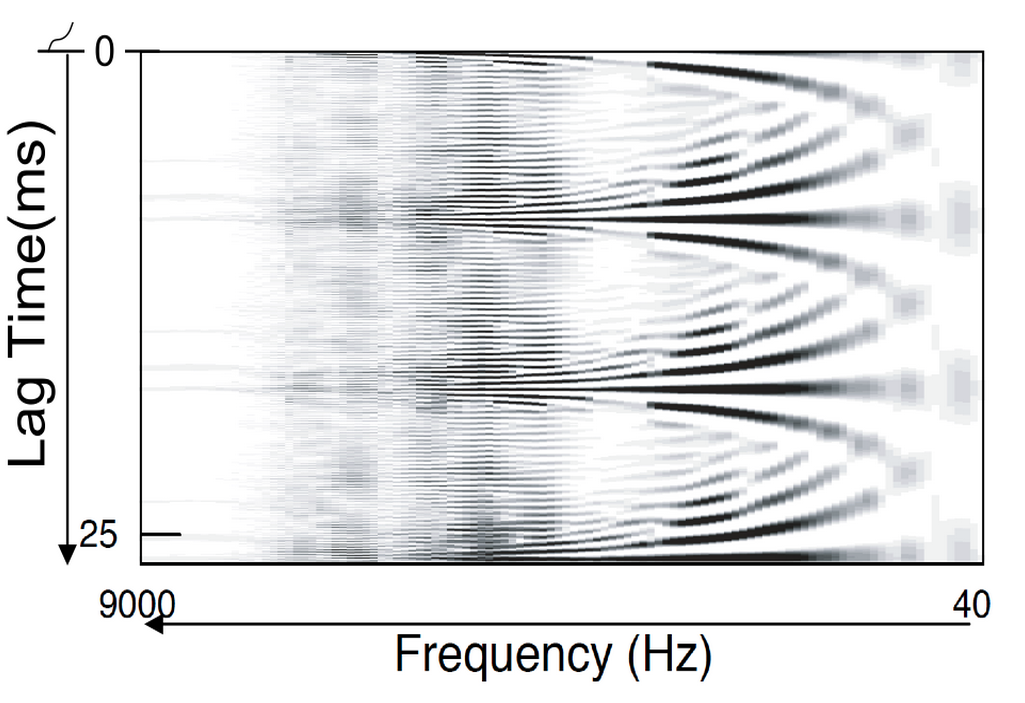
\includegraphics[width=150mm]{figures/sai}
%% \caption{Stabilized Auditory Image \label{fig:sai}}
%% \end{figure}

%% This SAI image representation generates a 2D image of each section of
%% samples from an audio file.  We then reduce this large amount of
%% information in two steps, first by cutting the image into overlapping
%% boxes and finding row and column residuals of these boxes, and then by
%% vector quantizing the resulting high dimensionality vector.  The
%% resulting spare vector is then histogrammed across the audio file, and
%% this histogram is then used as input to an SVM \cite{yh05}
%% classifier\cite{chapelle2006}.

%% The field of Music Information Retrieval (MIR) or Machine Hearing
%% \cite{marsyas} attempts to teach computers to understand music.  There
%% are a wide variety of tasks in this field that range from music
%% playlisting to analyzing Gregorian chants and Bach fugues.  Both in my
%% group at UVIC and at Google, we are specifically interested in
%% approaches that take audio as input.  From this audio we calculate a
%% variety of features, including the low, medium and high frequency
%% content and how these frequencies evolve over time.  We then use
%% advanced machine learning algorithms including Support Vector Machines
%% and Deep Belief Networks \cite{bengio2007}.

%% Most current approaches in MIR use spectral based approaches that use
%% the Fast Fourier Algorithm to decompose a signal into a set of
%% sinusoid's with a specific frequency and phase.  An example
%% spectrogram of a human voice is shown in Figure \ref{fig:spectrogram}.
%% These approaches are computationally efficient and fast, and give us a
%% good understanding of many features of music.  Using these features,
%% the field of MIR has had many successes, in the field of genre
%% recognition, for example, we often can achieve a classification
%% accuracy of 80\%.  In the past 5 years, most of the advances in MIR
%% have come from applying more and more advanced machine learning
%% algorithms to this problem.  It now appears that we have reached a
%% plateau where the performance of these systems is not increasing, and
%% it is felt that by using better audio features, performance can be
%% again improved.

%% FFT based approaches are fundamentally different from how our ear
%% actually hears sound.  FFT approaches take a window of data and
%% decompose this window into different sinusoids with a period and
%% phase.  The choice of window size involves a tradeoff between time
%% resolution and frequency resolution, and in order to increase time
%% resolution, frequency resolution must be decreased.  For certain
%% sounds produced in music, like those of sustained notes, this model
%% works well, but for many others, such as drum hits or the pulse
%% resonance phenomenon found in human voices, this model has
%% limitations.

%% The models of the human auditory system (Figure \ref{fig:humanear}
%% developed both by Dick Lyon \cite{slaney93} and other researchers
%% around the world have a fundamentally different approach in which
%% audio is filtered by a filterbank cascade that models features of the
%% human cochlea, the outputs of these filters are then processed by a
%% mechanism that is modeled on higher levels in the auditory periphery
%% that take this filterbank audio and generate two dimensional movie
%% frames that contain both frequency and an autocorrelation axis.  These
%% frames contain the fine timing information that is utilized by the
%% human hearing system to separate, localize and identify sounds.

%% This model finds trigger points in the input audio signal and
%% stabilizes the train of peaks from the CARFAC filterbank cascade into
%% a two dimensional image.  The output of the CARFAC filterbank is shown
%% in Figure \ref{fig:nap}, in this figure, the vertical axis corresponds
%% to cochlear place, with points closer to the bottom axis corresponding
%% to lower frequencies and the horizontal axis corresponding to time.
%% This plot can also be referred to as a Neural Activity Profile (NAP).
%% These peaks flow by rapidly, at the rate of pulses from the organism
%% in question, and in order to view them, one should align subsequent
%% peaks to each other.  There are many approaches to doing this, and the
%% approach commonly used is to find trigger points in the audio, that
%% is, points that correspond to pulses in the output of the vocal tract.
%% One trigger detection algorithm is shown schematically in Figure
%% \ref{fig:triggerpoints}.  In this figure the solid black line in the
%% center corresponds to the audio signal, and the red dots signify
%% trigger points.  The solid black line at the top of the figure
%% represents the current threshold value of the algorithm, and when this
%% threshold crosses the line representing the audio, a new trigger point
%% is generated.

%% In this section, we focus on retrieval rather than classification and
%% only use the ground truth labels as a way to measure retrieval
%% effectiveness. We compare different strategies over a large dataset
%% (185 calls, 4 classes) using well established retrieval effectiveness
%% measures. To the best of our knowledge this is the first systematic
%% evaluation of these different design choices.

%% \subsection{PZFC and CARFAC}
%% The CARFAC model includes a more advanced treatment of the fast acting
%% compression that the Outer Hair Cells in the cochlea perform to allow
%% the ear to hear both very loud and very soft sounds, a technique
%% formally referred to as Automatic Gain Control (AGC).  This model is
%% more advanced than the PZFC model, and this additional complexity can
%% be seen in Figure \ref{fig:dspcarfac}.

%% \begin{figure}[t]
%% \begin{center}
%% 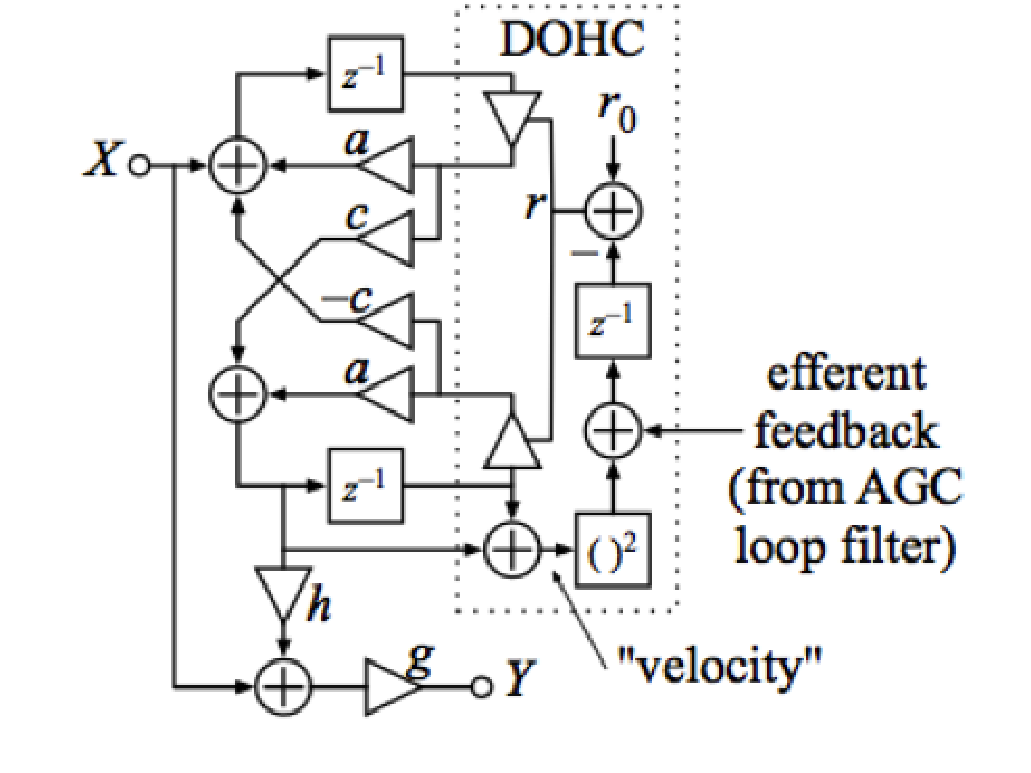
\includegraphics[width=50mm]{figures/dspcarfac}
%% \caption{
%% The Cascade of Asymmetric Filters and Resonators (CARFAC) model.  This
%% model is similar to the PZFC model, but includes an Automatic Gain
%% Control (AGC) stage, that models the action of the Outer Hair Cells in
%% the human cochlea.} 
%% \label{fig:dspcarfac} 
%% \end{center} 
%% \end{figure} 


%% The code for the CARFAC model was written in MATLAB, and it was my
%% task to take this code, port it to C++, verify that it worked
%% identically to the original code and then to optimize it to run as
%% quickly as possible.  For this, I used a software development
%% methodology called Test Driven Development \cite{fraser03} (TDD).  In
%% TDD, one inverts the normal software development process in that one
%% first writes the tests, and then the minimum code to make these tests
%% pass.  This is an ideal development strategy to use in this case,
%% since we have a working reference implementation of the algorithm in
%% MATLAB.  Using this strategy, I was able to port this MATLAB code
%% first to Python and then to C++.  The C++ code was added to the
%% Marsyas \cite{marsyas} framework and was open-sourced during my time
%% at Google, and is now available to be used by the community.

%% The process of porting the CARFAC model was straightforward but time
%% consuming.  After I had ported this model to C++, we then went back to
%% MATLAB to develop a model of binaural hearing using the output of the
%% CARFAC filter cascade.  We used the Stabilized Auditory Image (SAI) model
%% proposed by Patterson \cite{patterson92}, which works well for the
%% pulse resonance sounds created by many types of animals, from fish to
%% insects to the human voice.  In Figure \ref{fig:pulseresonance} the
%% sounds from various animals are shown, an in each one, the same
%% phenomenon is seen, where a fast impulse, or pulse is created and is
%% then resonated through the vocal tract or other sound producing organ
%% in the creature.

%% \begin{figure}[t]
%% \begin{center}
%% 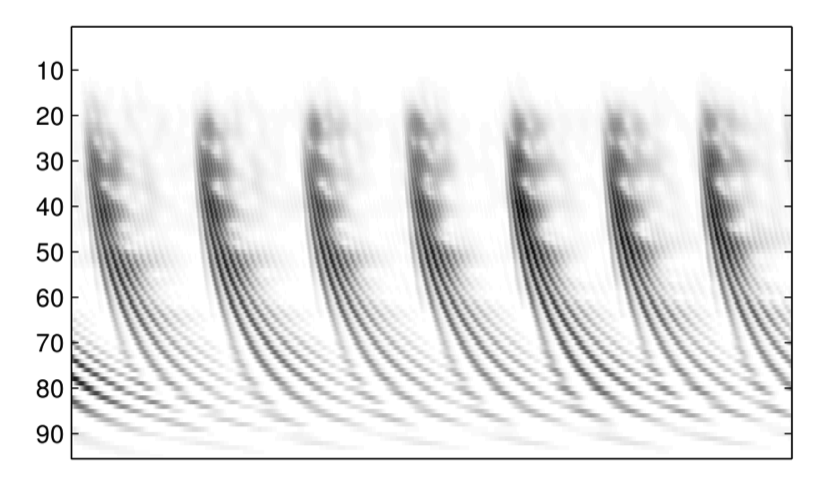
\includegraphics[width=100mm]{figures/nap}
%% \caption{ The Neural Activity Pattern (NAP) of the CARFAC model.  In
%%   this figure, the vertical axis corresponds to cochlear place, with
%%   points closer to the bottom axis corresponding to lower frequencies
%%   and the horizontal axis corresponding to time}
%% \label{fig:nap} 
%% \end{center} 
%% \end{figure} 

%% \begin{figure}[t]
%% \begin{center}
%% 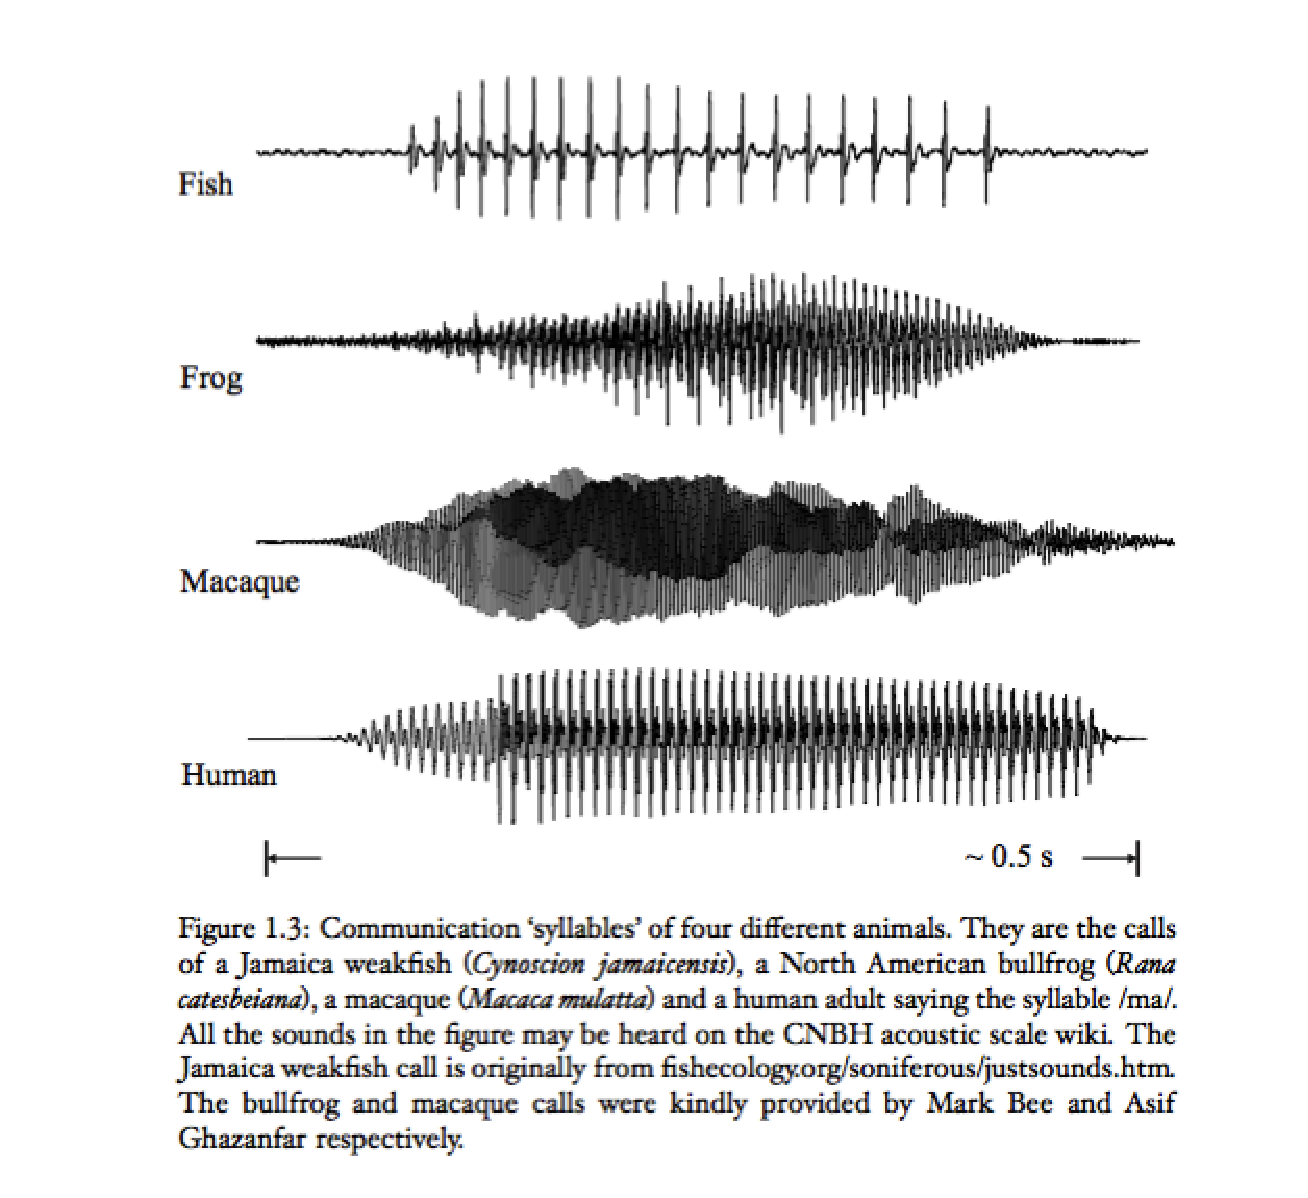
\includegraphics[width=100mm]{figures/pulseresonance}
%% \caption{ A diagram of the waveforms produced by a variety of
%%   different animals, showing the pulse and resonance structure of
%%   these vocalizations.  In each, a short pulse is generated which then
%%   reverberates through the vocal tract or sound producing organ of the
%%   organism.}
%% \label{fig:pulseresonance} 
%% \end{center} 
%% \end{figure} 

%% This model finds trigger points in the input audio signal and
%% stabilizes the train of peaks from the CARFAC filterbank cascade into
%% a two dimensional image.  The output of the CARFAC filterbank is shown
%% in Figure \ref{fig:nap}, in this figure, the vertical axis corresponds
%% to cochlear place, with points closer to the bottom axis corresponding
%% to lower frequencies and the horizontal axis corresponding to time.
%% This plot can also be referred to as a Neural Activity Profile (NAP).
%% These peaks flow by rapidly, at the rate of pulses from the organism
%% in question, and in order to view them, one should align subsequent
%% peaks to each other.  There are many approaches to doing this, and the
%% approach commonly used is to find trigger points in the audio, that
%% is, points that correspond to pulses in the output of the vocal tract.
%% One trigger detection algorithm is shown schematically in Figure
%% \ref{fig:triggerpoints}.  In this figure the solid black line in the
%% center corresponds to the audio signal, and the red dots signify
%% trigger points.  The solid black line at the top of the figure
%% represents the current threshold value of the algorithm, and when this
%% threshold crosses the line representing the audio, a new trigger point
%% is generated.

%% \begin{figure}[t]
%% \begin{center}
%% 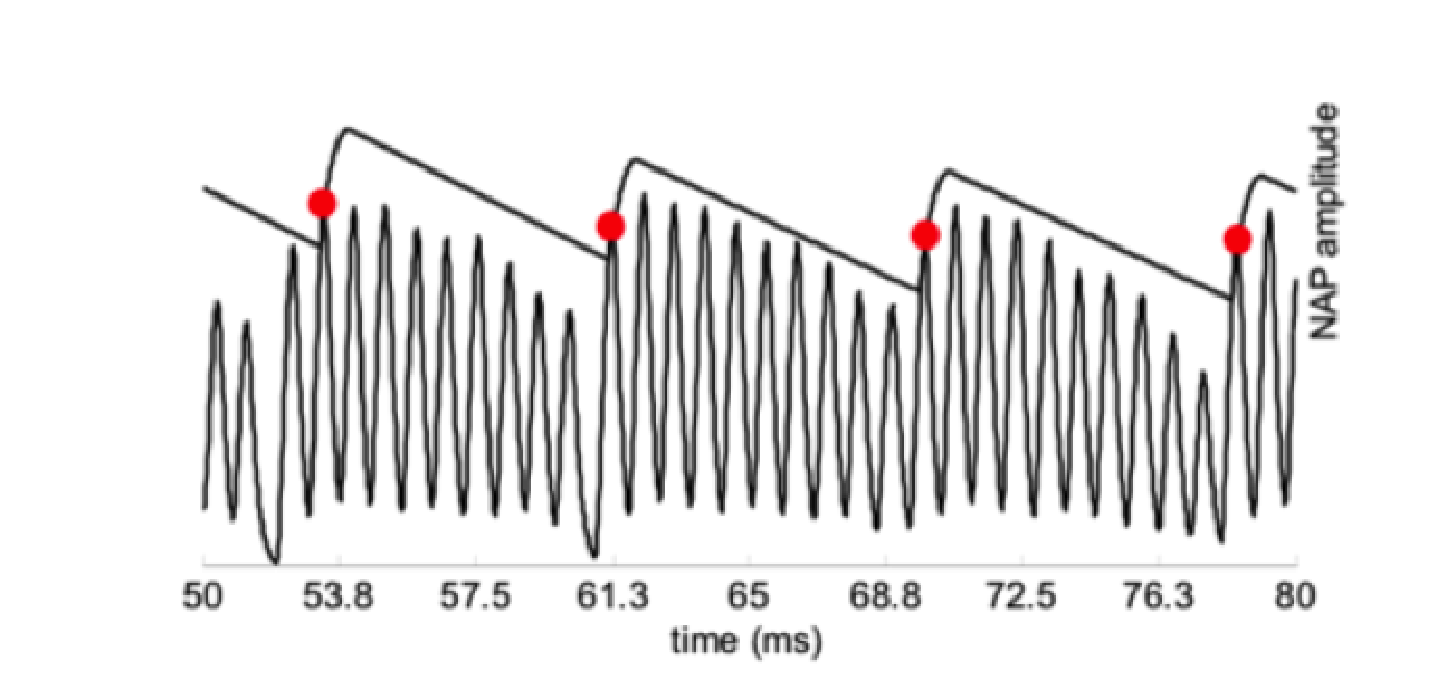
\includegraphics[width=100mm]{figures/triggerpoints}
%% \caption{ In this figure the solid black line in the center
%%   corresponds to the audio signal, and the red dots signify trigger
%%   points.  The solid black line at the top of the figure represents
%%   the current threshold value of the algorithm, and when this
%%   threshold crosses the line representing the audio, a new trigger
%%   point is generated.}
%% \label{fig:triggerpoints} 
%% \end{center} 
%% \end{figure} 

%% \begin{figure}[t]
%% \begin{center}
%% 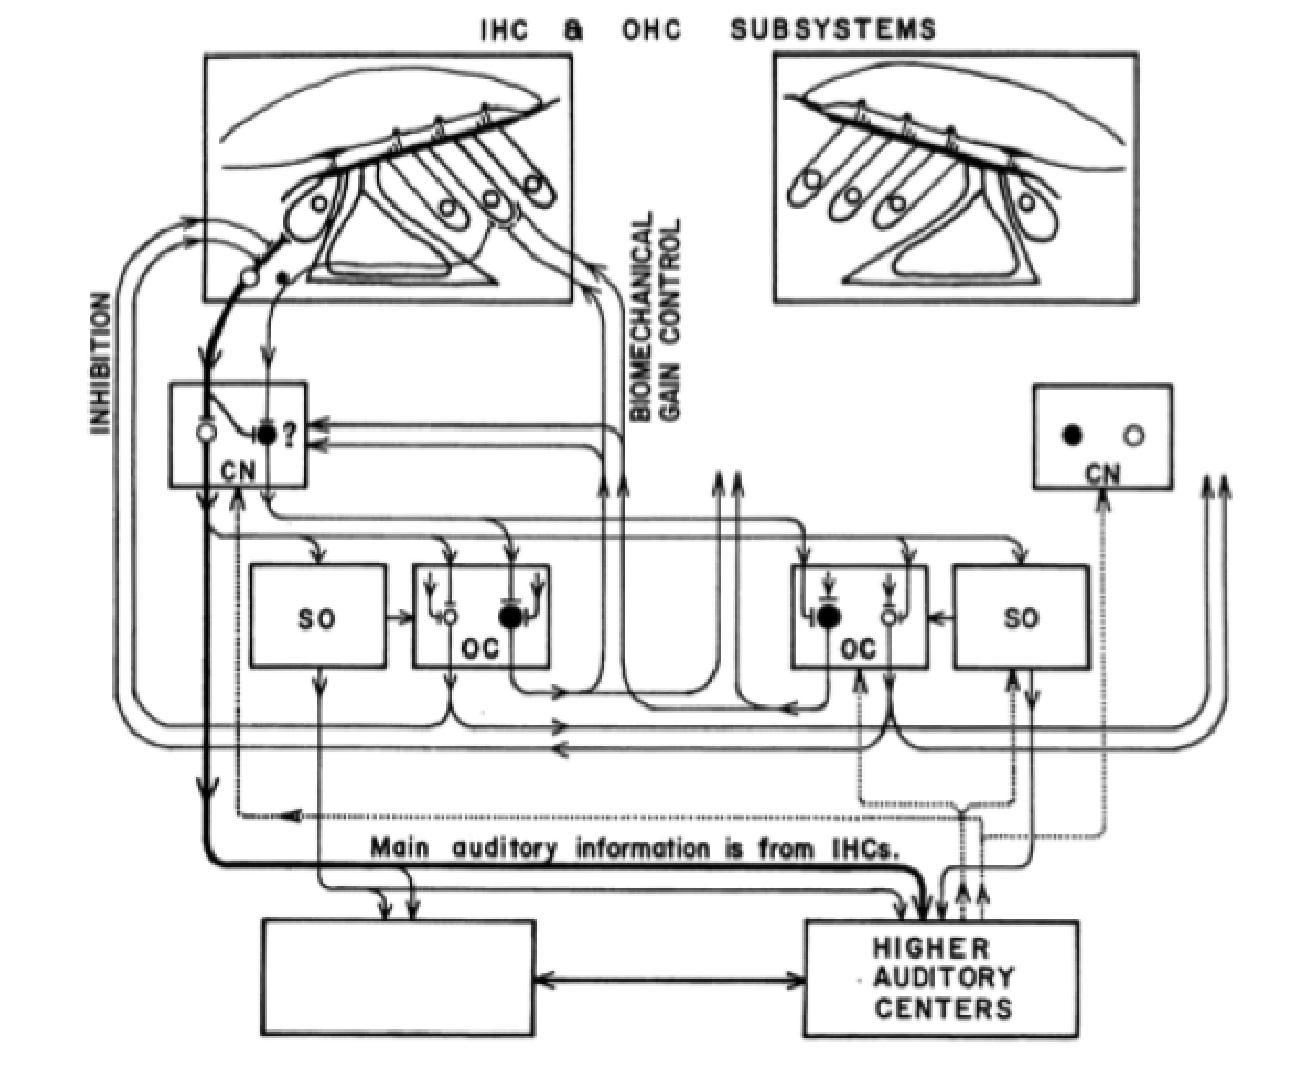
\includegraphics[width=100mm]{figures/ihcohc}
%% \caption{
%% A schematic view of the connections between the cochlea and the higher
%% levels of the auditory periphary, including connections between the
%% olivary complexes to each other and back to their respective cochleas.} 
%% \label{fig:ihcohc} 
%% \end{center} 
%% \end{figure} 

%% \subsubsection{SOM}

%% For creating the visualization layout we utilized the self-organizing
%% map (SOM) which is a type of neural network used to map a high
%% dimensional feature space to a lower dimensional representation while
%% preserving the topology of the high dimensional space. This
%% facilitates both similarity quantization and visualization
%% simultaneously. The SOM was first documented in 1982 by T. Kohonen,
%% and since then, it has been applied to a wide variety of diverse
%% clustering tasks \cite{kohonen95a}. In our system the SOM is used to
%% map the audio features (64-dimensions) corresponding to each track to
%% two discrete coordinates on a grid.

%% The traditional SOM consists of a 2D grid of neural nodes each
%% containing a $n$-dimensional vector, $ {\bf x(t)} $ of data. The goal
%% of learning in the SOM is to cause different neighbouring parts of the
%% network to respond similarly to certain input patterns. The network
%% must be fed a large number of example vectors that represent, as
%% closely as possible, the kinds of vectors expected during mapping. The
%% data associated with each node is initialized to small random values
%% before training. During training, a series of $n$-dimensional vectors
%% of sample data are added to the map.  The ``winning'' node of the map
%% known as the {\it best matching unit} (BMU) is found by computing the
%% distance between the added training vector and each of the nodes in
%% the SOM. This distance is calculated according to some pre-defined
%% distance metric which in our case is the standard Euclidean distance
%% on the normalized feature vectors.

%% Once the winning node has been defined, it and its surrounding nodes
%% reorganize their vector data to more closely resemble the added
%% training sample.  The training utilizes competitive learning. The
%% weights of the BMU and neurons close to it in the SOM lattice are
%% adjusted towards the input vector. The magnitude of the change
%% decreases with time and with distance from the BMU. The time-varying
%% learning rate and neighborhood function allow the SOM to gradually
%% converge and form clusters

%% For the Machine Learning half of the project, a variety of Machine
%% Learning systems and algorithms were used and comparison of them in is
%% provided in the evaluation section.  Results have been produced for a
%% Logistic Regression system using a Stochastic Gradient Descent
%% algorithm on Mahout, a distributed Machine Learning system implemented
%% as a Java library on top of Hadoop, an open source clone of the Google
%% File System (GFS) and Google MapReduce system.  These results are
%% compared to a Logistic Regression system using a quasi Newton solver
%% as implemented in Weka, a popular system for Machine Learning and show
%% timing and classification results of this system run as a grid style
%% parallel job on Westgrid.  These results for Logistic Regression are
%% then compared to three different implementations of a Support Vector
%% Machine (SVM) classifier.  The first of these is simply the SVM mode
%% in Weka but run in a grid-style distributed manner.  The second of
%% these is a parallel version of the SVM algorithm, PSVM
%% \cite{chang07psvm}.  The third of these is a hybrid audio feature
%% extraction and SVM developed in the Marsyas framework.  These three
%% different systems will be compared and contrasted in the Evaluation
%% section.

%% I propose to use the Westgrid system for running the huge audio
%% feature extraction task. This uses a very simple queuing system known
%% as Torque, which is the latest evolution of the ancient PBS (Parallel
%% Batch System) parallel job distribution system. PBS allows scientific
%% users to schedule large jobs to run on computers, and performs well
%% for certain scientific tasks where a single, usually large, program is
%% run on a variety of different datasets, and the results are then saved
%% to disk and later analyzed by a scientist. This type of computing was
%% traditionally known as Grid Computing.  While this system has certain
%% benefits for running specific scientific tasks, for other tasks, the
%% methodology of having separate computers running mostly independently,
%% and all coordination of tasks being the responsibility of the
%% programmer with an tool such as MPI quickly becomes difficult. The
%% MapReduce paradigm helps in the coordination of large parallel tasks,
%% and the Hadoop system allows programmers to efficiently write
%% distributed programs that run on huge numbers of computers and allows
%% for failures of individual computers. In this project we will use the
%% Mahout Machine Learning framework on top of a Hadoop installation to
%% process the audio feature vectors output by Marsyas and to gain
%% insights into the vocalization data in the Orchive. The primary task I
%% will investigate in this project will be identifying regions of the
%% Orchive with distinct orca vocalizations that are nearby to
%% hydrophones and isolated from other orca vocalizations.

%% Mahout is a Machine Learning framework that interacts closely with
%% Hadoop to both store the data and also run the Machine Learning
%% algorithms.  Hadoop is an open source port of the GFS
%% \cite{ghemawat03} and MapReduce \cite{dean08} infrastructure and
%% allows users to run large jobs that follow the map reduce paradigm.
%% In this scheme, a parallel job is split into two phases, a map phase
%% and a reduce phase.  In the map phase, key value pairs are generated
%% by some given algorithm from an input file, this same process occurs
%% in parallel on many other nodes, and the data that is used by a given
%% map is determined by the locality of data on that node.  These key
%% value pairs are then sorted and shuffled to a set of reduce nodes,
%% which take the collections of key value pairs and do an operation on
%% them that in some way combines, or reduces, the data.  These map and
%% reduce functions can be thought of as similar to the map and reduce
%% functions in functional programming, however, it should be noted that
%% this is a loose similarity due to the lack of higher order functions
%% in the current MapReduce implementation.  Many algorithms have been
%% ported to use this MapReduce type system, some of the most natural are
%% those that process large collections of text for building inverted
%% indexes or other tasks for searches, which is not surprising noting
%% the provenance of the MapReduce algorithm.  For other tasks, such as
%% those common in audio feature extraction, the reduce phase is simply
%% an identity reduce, where the map outputs are copied verbatim to the
%% reduce outputs.  It is easier and more natural to make some algorithms
%% more efficient in a MapReduce context than others.

%% The Mahout Machine Learning framework has implemented many different
%% Machine Learning algorithms in it's framework, including clustering,
%% recommendation and classification algorithms.  In our current work we
%% are more interested in classification than either recommendation or
%% clustering, and Mahout boasts support for the following classification
%% algorithms: Logistic Regression (SGD), Bayesian, Support Vector
%% Machines (SVM), Perceptron and Winnow, Neural Network, Random Forests,
%% Restricted Boltzmann Machines, Online Passive Aggressive, Boosting and
%% Hidden Markov Models.  However, after investigation, it appears most
%% of these algorithms are in a definite alpha state, and require
%% patching of the main source tree with external files.  The two most
%% well supported classification algorithms in Mahout are the Logistic
%% Regression classifier, using a Stochastic Gradient Descent (SGD)
%% engine, and a Naive Bayesian classifier.  Upon extensive
%% investigation, the Bayesian classifier makes many internal assumptions
%% of the input being of large bodies of written text and was not
%% suitable for our use case.  However, the Logistic Regression
%% classifier was well suited to our data and performed well in our
%% tests.

%% One advantage of using the Mahout Machine Learning framework was that
%% it stored its input and output data on HDFS, the Hadoop Distributed
%% Filesystem.  When working with the huge amounts of data that are
%% generated by audio feature extraction and Machine Learning
%% experiments, managing and transferring experimental results from the
%% grid servers to the production web servers is often a time consuming
%% and error prone procedure.  After our experience with Hadoop, we have
%% integrated it into web application and use the WebHDFS system to serve
%% all experimental results to users.  These users interact with a web
%% application that displays some data obtained from the production web
%% server but also displays the results of experiments as data served
%% live from a WebHDFS system that is being populated by the experimental
%% results from live requests from scientists.


%% , the porting from
%% MATLAB of the various subsystems required for the calculation of
%% Stable Auditory Images (including the Pole Zero Filter Cascade,
%% Gammatone filterbank, CARFAC, Halfwave Rectification, Stable Auditory
%% Image, Scale Stabilized Auditory Image, Box cutting, and Vector
%% Quantization), and the development and implementation of a Sideband
%% Interval detector.

%% %
%% % Stabilized auditory image
%% %

%% Another type of feature that could be used for call detection is the
%% Stablised Auditory Image.  

%% - Brief description of SAI
%% - Diagram of SAI generation

%% - Different filterbanks to use - Gammatone, PZFC, CARFAC.  These are
%% all progressively more detailed models of the cochlea, and model both
%% the filtering processes within the cochlea as well as the automatic
%% gain control mechanism in the mechanical cochlea.

%% The filterbank is followed by a halfwave linear rectification
%% algorithm which models the way that inner hair cells communicate with
%% neurons.  In this process, there is a electochemical gradient between
%% the two sides of membrane the inner hair cell is attached to, and when
%% the inner hair cell flexes in the forward direction, it physically
%% opens a channel that allows ions to pass, and when it flexes in the
%% reverse direction, this channel closes.  This gives a signal that is
%% similar to a half-wave rectified filter, in which only the positive
%% part of the signal is transmitted, and the negative part is made zero.

%% This is followed by a strobe detector, which looks for a local maximum
%% in the signal, and when a certain threshold has been detected, it
%% sends the signal to the next stage in the pipeline.  This local
%% maximum has a decaying threshold with a timeout, so that strobes are
%% guaranteed to be delivered at a certain rate, even if the signal is at
%% a low value.


%% - Different 
%% - Gives clear patterns on image when audio with a pulsed nature is
%%   used as input
%% - Show frames of SAI movie showing the different sections of audio and
%%   how well they work




%% \begin{table}
%% \begin{tabular}{|l|l|l|}
%% \hline


%% \hline
%% \end{tabular}
%% \caption{}
%% \label{table:obv-6-SAI}
%% \end{table}




%
% Downsampling
%



%% %
%% % Spectrogram cross-correlation
%% %


%% Another method that is used for call detection is spectrogram
%% cross-correlation, where a kernel is used to

%% - Description of Spectrogram Cross-correlation
%% - Take spectrograms of call catalog as kernels
%% - Run each kernel over the spectrogram


%% \begin{table}
%% \begin{tabular}{|l|l|l|l|l|}
%% \hline
%% Window Size & Hop Size & Memory & Total feature vectors & Percent Correct \\
%% \hline


%% \hline
%% \end{tabular}
%% \caption{Table of downsampling 100 (or whatever is reasonable) with weka with
%% MFCC + Spectral with different}
%% \label{table:mfccSpectralWeka}
%% \end{table}





%% %
%% % Voting
%% %

%% The previous experiments were on a feature by feature basis.  The
%% pulsed calls made by orcas extend over a span of time, typically from
%% 0.5 to 3 seconds in length, and we can take advantage of this fact by
%% using a window in which the classifications of individual feature
%% vectors can be combined using a voting paradigm.  In this experiment,
%% all the orca, background and voice clips were concatenated together
%% in order to approximate the continuous nature of the actual sounds to
%% be classified.

%% \begin{table}
%% \begin{tabular}{|l|l|l|}
%% \hline
%% \# of frames & Percent Correct \\
%% \hline


%% \hline
%% \end{tabular}
%% \caption{Table of spectral features with voting per slice}
%% \label{table:obvVoting}
%% \end{table}


%
% Image compression
%

%% \subsection{Image compression}


%% - Description of Image compression to find calls
%% - Use call catalog as kernels
%% - Spectrogram used as 

%% \begin{table}
%% \begin{tabular}{|l|l|l|l|l|}
%% \hline
%% Window Size & Hop Size & Memory & Total feature vectors & Percent Correct \\
%% \hline


%% \hline
%% \end{tabular}
%% \caption{Table of downsampling 100 (or whatever is reasonable) with weka with
%% MFCC + Spectral with different}
%% \label{table:mfccSpectralWeka}
%% \end{table}


%% %
%% % Dynamic Time Warping
%% %

%% \subsection{Dynamic Time Warping}


%% - Description of Dynamic Time Warping (DTW)
%% - Similar to spectrogram cross-correlation but also takes into account
%%   time differences
%% - Expensive for doing call detection


%% \begin{table}
%% \begin{tabular}{|l|l|l|}
%% \hline

%% \hline


%% \hline
%% \end{tabular}
%% \caption{SBI}
%% \label{table:obvSBI}
%% \end{table}

%
% Standard MIR features
%




%
% Spectrogram cross correlation
%





%
% Image compression
%





%
% Dynamic Time warping
%




%
% Vector quantization and SAX/bioinformatics
%





%
% Stabilized auditory images
%





%
% Deep belief networks on spectrograms
%

%% \subsection{Mahout}


%% \section{Distributed Computation}


%% \subsection{Grid Computing}


%% \begin{bchart}[max=50]
%% \bcbar{45}
%% \bcbar{26}
%% \bcbar{31}
%% \label{bchart:test1}
%% \end{bchart}

%% \section{Audio Feature Extraction and Machine Learning}

%% We performed an experiment in which we examined a quantitative ranking
%% task over a diverse set of audio files using tags associated with the
%% audio files.

%% In order to estimate the performance of the learned ranker, we used a
%% standard three-fold cross-validation experimental setup.  In this
%% scheme, two thirds of the data is used for training and one third is
%% used for testing; this process is then repeated for all three splits
%% of the data and results of the three are averaged.  We removed any
%% queries that had fewer than 5 documents in either the training set or
%% the test set, and if the corresponding documents had no other tags,
%% these documents were removed as well.

%% We evaluated our learned model by looking at the precision within the
%% top k audio files from the test set as ranked by each query.
%% Precision at top k is a commonly used measure in retrieval tasks such
%% as these and measures the fraction of positive results within the top
%% k results from a query.

%% The stabilized auditory image generation process has a number of
%% parameters which can be adjusted including the parameters of the PZFC
%% filter and the size of rectangles that the SAI is cut into for
%% subsequent vector quantization.  We created a default set of
%% parameters and then varied these parameters in our experiments.  The
%% default SAI box-cutting was performed with 16 lags and 32 channels,
%% which gave a total of 49 rectangles.  These rectangles were then
%% reduced to their marginal values which gives a 48 dimension vector,
%% and a codebook of size 256 was used for each box, giving a total of 49
%% x 256 = 12544 feature dimensions.  Starting from these, we then made
%% systematic variations to a number of different parameters and measured
%% their effect on precision of retrieval.  For the box-cutting step, we
%% adjusted various parameters including the smallest sized rectangle,
%% and the maximum number of rectangles used for segmentation.  We also
%% varied the codebook sizes that we used in the sparse coding step.

%% In order to evaluate our method, we compared it with results obtained
%% using a very common feature extraction method for audio analysis,
%% MFCCs (mel-frequency cepstral coefficients).  In order to compare this
%% type of feature extraction with our own, we turned these MFCC
%% coefficients into a sparse code.  These MFCC coefficients were
%% calculated with a Hamming window with initial parameters based on a
%% setting optimized for speech.  We then changed various parameters of
%% the MFCC algorithm, including the number of cepstral coefficients (13
%% for speech), the length of each frame (25ms for speech), and the
%% number of codebooks that were used to sparsify the dense MFCC features
%% for each frame.  We obtained the best performance with 40 cepstral
%% coefficients, a window size of 40ms and codebooks of size 5000.

%% We first preprocessed a collection of 1000 music files from 10 genres
%% using a PZFC filterbank followed by strobed temporal integration to
%% yield a set of SAI frames for each file .  We then take this set of
%% SAI and apply the box-cutting technique described above. The followed
%% by the calculation of row and column marginals.  These vectors are
%% then used to train dictionaries of 200 entries, representing abstract
%% ``auditory words'', for each box position, using a k-means algorithm.

%% This process requires the processing of large amounts of data, just to
%% train the VQ codebooks on a training corpus.

%% The resulting dictionaries for all boxes are then used in the MIREX
%% experiment to convert the dense features from the box cutting step on
%% the test corpus songs into a set of sparse features where each box was
%% represented by a vector of 200 elements with only one element being
%% non-zero.  The sparse vectors for each box were then concatenated, and
%% these long spare vectors are histogrammed over the entire audio file
%% to produce a sparse feature vector for each song or sound effect.
%% This operation of constructing a sparse bag of auditory words was done
%% for both the training and testing corpora.

%% \subsection{Audio Feature Extraction}

%% Our evaluation section consists of three parts, in the first we
%% optimize basic audio feature extraction parameters, in the second we
%% use different distributed Machine Learning systems to generate
%% classification results, and in the third we give a report on our
%% experiences with these different platforms for feature extraction and
%% Machine Learning.

%% Our first challenge when dealing with the Orchive is the huge size of
%% the data.  The raw uncompressed .wav files that were digitized from
%% tape take approximately 12TB on disk at the time of this analysis,
%% with more files being added all the time.  In order to determine if we
%% could use a compressed format for doing the audio feature extraction,
%% we compared the results of using a SVM machine to classify the frames
%% of audio.  For the original .wav file we got a classification accuracy
%% of 94.5\%, while a highly compressed 32kbs MP3 gave 93.6\% accuracy.
%% The disk quota on the Westgrid system is set by default at 1TB, so by
%% sacrificing a small amount of accuracy, it was possible to reduce the
%% disk space used from 12TB to 199GB, a 60x savings in space.

%% In order to test the different distributed audio classification
%% systems we first generated a set of training and testing data.  In a
%% previous paper \cite{ness2008}, we were able to obtain a
%% classification performance of 82\% when using a SVM classifier on hand
%% labelled data.  While this performance was adequate when used on a
%% small recording, when run on the entire Orchive, this performance
%% would lead to way too many false positives.  For this paper, we looked
%% in more detail at the training data, and found that while the
%% annotation boundaries were close to the start and end of the
%% vocalization, there was a small amount of silence before and after the
%% vocalization.  Using Audacity, we trimmed out all the silences of a 10
%% second region of audio of orca vocalizations, and did the same to a 10
%% second region of voice notes.  For the background data, we took one
%% hundred 0.1 second regions from random background annotations and
%% joined them together with the Linux audio utility program sox.  The
%% results for this can be found in the first line of table
%% \ref{table:handTrimmed} and had over 99.73\% of the instances
%% classified correctly.  This large jump in performance was unexpected
%% but easily understood, because if feature vectors of silence are
%% labelled as orca, this will cause issues for the classifier.  We then
%% took a 4 minute region of orca calls and voice notes and removed all
%% the silences from both of them.  We then did a preliminary test where
%% we reduced computation time by downsampling the feature vectors at a
%% rate of 100:1, this is shown in the next line of Table
%% \ref{table:handTrimmed}, and followed this by another test at 10:1
%% downsampling and one with no downsampling.  These tests gave
%% classification performance of 95.7\% to 97.7\%.  We then repeated the
%% analysis in our previous paper by using non-hand-trimmed audio, the
%% results are shown in the third section of the table.  We found results
%% from 88.1\% to 93.0\% for 100:1 and no downsampling.  The difference
%% of this result from the previous paper is likely due to the exact
%% training and testing sets used in the two papers.  In the current
%% paper, we are classifying only nearby and isolated orca vocalizations
%% and not the distant or noisy vocalizations, which was a small tweak to
%% the experimental setup that has also helped us to not only achieve
%% better classification performance but to deliver a science goal more
%% pertinent to the bioacoustics researchers who could use the Orchive.

%% \begin{table}
%% \begin{tabular}{|l|c|l|l|r|r|}
%% \hline
%%  trim & time (min)  & ds & features & \# & \% corr.  \\
%% \hline
%%  x & 10 sec  &  1   & all   &    2586  &    99.73  \\
%% \hline
%%  x & 4       & 100  & all   &     606  &    95.71  \\
%%  x & 4       & 10   & all   &    6060  &    97.19  \\ 
%%  x & 4       & 1    & all   &   60596  &    97.72  \\
%%  x & 4       & 100  & mfcc  &     606  &    94.88  \\
%%  x & 4       & 10   & mfcc  &    6060  &    96.03  \\
%%  x & 4       & 100  & yin   &     606  &    xx.xxxx  \\
%%  x & 4       & 10   & yin   &    6060  &    xx.xxxx  \\
%% \hline
%%    & 4       & 100  & all   &     621  &    88.08  \\
%%    & 4       & 10   & all   &    6202  &    92.26  \\
%%    & 4       & 1    & all   &   62023  &    93.01  \\
%%    & 4       & 100  & mfcc  &     621  &    87.76  \\
%%    & 4       & 10   & mfcc  &    6202  &    91.52  \\
%% \hline
%% \end{tabular}
%% \caption{Classification results with hand trimmed orca vocalizations
%%   using bextract to generate audio features and the SVM classifier in
%%   Weka to do a 10-fold crossvalidation of these features.}
%% \label{table:handTrimmed}
%% \end{table}

%% The next task that we worked on was to determine the optimal settings
%% for the audio extraction algorithm.  While there are a number of other
%% audio extraction frameworks in existence like jMIR \cite{mckayphd},
%% SmIrK \cite{wang07} and AIMC \cite{waltersphd}, the Marsyas framework
%% implements most, if not all, of the most popular audio feature
%% extraction algorithms, and presents them as output from the
%% ``bextract'' program as .arff files, which are the input to the Weka
%% suite of Machine Learning programs.  For all experiments here, we use
%% the audio features calculated by Marsyas, however in the future it
%% would be desirable to integrate other audio processing frameworks
%% within OpenMIR.

%% The features output by bextract include the number of zero crossings
%% per unit time, three spectral descriptors (centroid, rolloff, flux),
%% Mel-Frequency Cepstral Coefficients (MFCC) and chroma information
%% based on the western equally tempered scale.  The mean and standard
%% deviation of each of these over a window is then calculated and forms
%% the output.  The first experiment we did was to determine if the MFCC
%% coefficients contained enough information to do the classification on
%% their own, the results for this are shown in Table
%% \ref{table:handTrimmed} in the columns with ``mfcc'' in the
%% ``features'' column.  For the hand trimmed example at a downsampling
%% of 10:1, the performance goes from 97.2\% to 96.0\% which is a small
%% but meaningful difference, especially when one considers how many more
%% false positives one would get when looking at the entire Orchive.  We
%% also tried adding the Yin pitch estimator as another feature in the
%% feature vector output by bextract.  Surprisingly, as one can see in
%% the previous table, the addition of this information actually degraded
%% performance of the classifier.  We are currently investigating how to
%% better incorporate pitch tracking information in our classifiers.

%% The next set of parameters that needed to be optimized were the Window
%% Size and Hop Size of the Digital Signal Processing (DSP) algorithms
%% that take the input audio and calculate spectral information from
%% them, the fundamental basis for which is the Fast Fourier Transform
%% (FFT) algorithm.  One other important input to the bextract feature
%% extraction algorithm is the length of time over which to calculate the
%% statistical properties of the features, this is known in bextract as
%% the ``memory'' and corresponds to the number of frames of features
%% that are accumulated.  The results for this are shown in Table
%% \ref{table:dspParams}.  From this we can see that as we go to longer
%% window sizes, the classification performance increases, and as we go
%% to longer accumulation window sizes, the performance also increases.

%% For our experiments we decided that a good sweet spot was a hop size
%% size of 1024 and a memory of 40 frames, which gave a classification
%% performance of 99.7\%.  80 frames of audio at a sampling rate of 44100
%% samples/sec and a hop size of 1024 would result in a feature length of
%% 1.86 seconds, while 40 frames would only give 0.93 seconds of audio
%% per feature.  Given that orca vocalizations are usually between 0.5
%% and 3 seconds long, we chose a window size of 2048, a hop size of 1024
%% with an accumulator memory of 40 frames.  We did extensive experiments
%% with other values of hopsize, window size and memory that were
%% consistent with these results that are too long to report here.

%% \begin{table}
%% \begin{tabular}{|r|r|r|r|r|r|}
%% \hline
%%  winsize  &  hopsize  &  memory  &  total &   correct  \\
%% \hline
%%      256  &      128  &      20  &        13767   &    97.11  \\
%%      512  &      256  &      20  &        11647   &    96.11  \\
%%     1024  &      512  &      20  &         5923   &    97.74  \\
%%     2048  &     1024  &      20  &         2995   &    98.84  \\
%% \hline
%%      256  &      128  &      40  &        23311   &    96.18  \\
%%      512  &      256  &      40  &        11829   &    97.61  \\
%%     1024  &      512  &      40  &         5991   &    98.86  \\
%%     2048  &     1024  &      40  &         3022   &    99.74  \\
%% \hline
%%      256  &      128  &      80  &        23628   &    97.48  \\
%%      512  &      256  &      80  &        11963   &    98.71  \\
%%     1024  &      512  &      80  &         6044   &    99.74  \\
%%     2048  &     1024  &      80  &         3027   &    99.90  \\
%% \hline
%% \end{tabular}
%% \caption{DSP parameters}
%% \label{table:dspParams}
%% \end{table}

%% \subsection{Machine Learning}

%% The main distributed Machine Learning framework we used was Mahout,
%% which as we previous described is a Java framework for Machine
%% Learning that operates on top of Hadoop.  We investigated a number of
%% its algorithms and found that the Logistic Regression algorithm was
%% the only classification algorithm that was both suitable for our
%% problem and incorporated into the main source code trunk of the code.
%% Our first experiment was just to test the two parameters suggested for
%% tuning this algorithm are shown in Table
%% \ref{table:logisticRegressionTests}, and from these brief experiments
%% it appears the default parameters work best on this data.

%% \begin{table}
%% \begin{tabular}{|r|r|l|}
%% \hline
%%  Passes  & Rate  & Percent Correct                                         \\
%% \hline
%%     100  &    50  &  85.5  \\
%%    1000  &    50  &  85.5  \\
%%     100  &     5  &  83.0  \\
%%     100  &   500  &  85.5  \\
%% \hline
%% \end{tabular}
%% \caption{Logistic regression tests with different parameters.}
%% \label{table:logisticRegressionTests}
%% \end{table}

%% We then took a randomly selected 13GB portion of the 500GB of total
%% (one of the original 37 shards from feature extraction) audio features
%% calculated in the previous section and ran a comparison of the Mahout
%% Logistic Regression algorithm against a simple parallel
%% implementation using a script that runs Weka jobs on multiple
%% computers using the Torque/PBS system on the Westgrid cluster.

%% For this we had our choice of a number of systems on which to run a
%% Mahout/Hadoop cluster on and investigated all of them.  The first was
%% Emulab, which is a fine platform and is very useful for a number of
%% use cases, but for this case of obtaining 10-20 computers and storing
%% substantial amounts of long lived data on them did not fit the Emulab
%% model of running distributed programs on different types of emulated
%% networks on short lived borrowed computers.  While it would have been
%% possible to use Emulab, we were hoping for a longer term solution.
%% Planetlab allows for longer leases, but the large memory and CPU
%% requirements of our program made this less feasible as well.  We
%% attempted to obtain machines on the GeniCloud at HP, but were unable
%% to obtain the machines in the end.  The best solution we felt was to
%% use the six GreenGeni nodes at UVIC and setup a Hadoop cluster on
%% these.  We attempted to do this for quite some time, but ran into a
%% number of odd port issues.  We suspect the problem are concurrently
%% running Swift and Disco installs on these machines that might be
%% utilizing these ephemerally used ports.  The problem could also be due
%% to a misconfiguration of the networking hardware.  Another solution
%% would be to use the Amazon EC2 cluster service, or even their Elastic
%% MapReduce service, a service that is easy to setup and use, however,
%% costs for it can add up quickly.  For the results in this paper we use
%% a mini 2-node Hadoop cluster that was setup in our lab in a controlled
%% setting, this was simple to install and get results from.  In the near
%% future we hope to setup a larger Hadoop cluster and to rerun these
%% jobs with more processors.

%% For all of our analysis here, we took one of the 37 splits of the
%% original data analyzed by bextract.  This file was 13GB in size and
%% contained 22486467 lines.  For the following experiments we took the
%% first $n$ lines of this file where $n$ started at 10 and increased to
%% 10,000,000 in powers of 10.

%% For the first experimental condition, the Logistic Regression
%% Classifier as implemented in Mahout was used, and Hadoop was used as
%% the underlying system below Mahout.  The Logistic Regression
%% classifier as implemented by default in Mahout can only take two
%% classes as input, so for all these experiments we used only orca and
%% background as the training data.  The timing results of Logistic
%% Regression in Mahout are shown in Table
%% \ref{table:machineLearningTiming1}.  As we can see, the system is very
%% fast, even classifying a million instances only takes one minute on a
%% small two node cluster.  As the number of instances increases, the
%% time increases quickly, it would be interesting to see this with a
%% larger cluster of 10 or more nodes.

%% For the second experimental condition, we used the Weka Machine
%% Learning package and ran it with it's Logistic Regression engine.
%% This was run on the Hermes cluster at Westgrid, and for these tests,
%% only 10 nodes were run at one time, although scaling up is as simple
%% as splitting the input file into more chunks and starting more jobs.
%% Weka is a Java program, and thus incurs a certain startup time when
%% creating and setting up the JVM and other resources.  This is
%% reflected in the results in Table \ref{table:machineLearningTiming2}
%% where up to 100000 instances the run times are all around 6 seconds.
%% The third experimental condition was to use Weka again, but this time
%% with its SVM engine.  Interestingly, the time that the SVM took to run
%% was about the same as the Logistic Regression, even though SVM is
%% typically be a considerably better classifier than Logistic
%% Regression.

%% In the final experiment, PSVM was run on the Checkers cluster at
%% Westgrid.  It was unable to be run on the Hermes and Nestor clusters
%% due to the use of MPICH2 by PSVM and the use of the original MPI
%% version 1.0 on the clusters.  This program takes advantage of the MPI
%% message passing library to communicate between a number of different
%% computers, and for the experiments shown below, we used 4 processors.
%% It should be noted that at least on the Checkers cluster, it is
%% difficult to reserve a block of 5 computers at once, much more
%% difficult than starting 5 individual jobs.  Depending on the cluster
%% you have access to, this may or may not be a problem.


%% \begin{table}
%% \begin{tabular}{|l|r|r|r|}
%% \hline
%%  system  &  \# proc.  &  num instances  &  time (sec)  \\
%% \hline
%%  Mahout  &     2          &            100  &       0.55  \\
%%  Mahout  &     2          &           1000  &       0.89  \\
%%  Mahout  &     2          &          10000  &       1.45  \\
%%  Mahout  &     2          &         100000  &       6.69  \\
%%  Mahout  &     2          &        1000000  &      57.90  \\
%%  Mahout  &     2          &       10000000  &     566.35  \\
%%  Mahout  &     2          &       22486467  &     566.35  \\
%% \hline
%%  PSVM     &           10  &            100  &     2  \\
%%  PSVM     &           10  &           1000  &     1  \\
%%  PSVM     &           10  &          10000  &     1  \\
%%  PSVM     &           10  &         100000  &     50  \\
%%  PSVM     &           10  &        1000000  &     635  \\
%%  PSVM     &           10  &       10000000  &       \\
%%  PSVM     &           10  &       22486467  &       \\
%% \hline
%% \end{tabular}
%% \caption{Timing results for all Machine Learning Algorithms}
%% \label{table:machineLearningTiming1}
%% \end{table}

%% \begin{table}
%% \begin{tabular}{|l|r|r|r|}
%% \hline
%%  system  &  \# proc.  &  num instances  &  time (sec)  \\
%% \hline
%%  Weka : LogReg    &           10  &            100  &        6.03  \\
%%  Weka : LogReg    &           10  &           1000  &        6.05  \\
%%  Weka : LogReg    &           10  &          10000  &        6.09  \\
%%  Weka : LogReg    &           10  &         100000  &        7.55  \\
%%  Weka : LogReg    &           10  &        1000000  &       31.24  \\
%%  Weka : LogReg    &           10  &       10000000  &      183.74  \\
%%  Weka : LogReg    &           10  &       22486467  &      233.99  \\
%% \hline
%%  Weka : SVM     &           10  &            100  &        5.38  \\
%%  Weka : SVM     &           10  &           1000  &        5.35  \\
%%  Weka : SVM     &           10  &          10000  &        5.15  \\
%%  Weka : SVM     &           10  &         100000  &        7.53  \\
%%  Weka : SVM     &           10  &        1000000  &       28.66  \\
%%  Weka : SVM     &           10  &       10000000  &      182.61  \\
%%  Weka : SVM     &           10  &       22486467  &      	  \\
%% \hline
%% \end{tabular}
%% \caption{Timing results for all Machine Learning Algorithms}
%% \label{table:machineLearningTiming2}
%% \end{table}


%% \section{Orca}

%% \begin{table}
%% \caption{Classification Performance}
%% \begin{tabular}{|c|c|c|} \hline

%% Dataset&Correctly Classified Instances&Percent Correct\\ \hline

%% 446A & 30403 & 90.31\\ \hline
%% 446B & 33701 & 81.97\\ \hline
%% 447B & 23013 & 73.65\\ \hline
%% 448A & 15307 & 58.04\\ \hline
%% 448B & 20822 & 74.61\\ \hline
%% 449B & 25239 & 81.17\\ \hline
%% 450A & 31872 & 87.85\\ \hline
%% 450B & 23916 & 93.51\\ \hline
%% 451A & 54281 & 89.74\\ \hline
%% 451B & 25528 & 69.91\\ \hline
%% \hline\end{tabular}
%% \end{table}


%% \begin{table}
%% \centering
%% \caption{Recording-specific classification performance}
%% \begin{tabular}{|c|c|c|c|c|} \hline

%% &\multicolumn{2}{|c|}{Naive bayes}&\multicolumn{2}{|c|}{SMO}\\
%% &\multicolumn{2}{|c|}{\% correct}&\multicolumn{2}{|c|}{\% correct}\\ \hline
%% &self&train with&self&train with\\
%% &&remaining&&remaining\\ \hline

%% 446A  &  89.42  &  93.10  &  95.00  &  73.39\\ \hline
%% 446B  &  63.45  &  77.66  &  85.85  &  70.23\\ \hline
%% 447B  &  75.46  &  57.32  &  82.02  &  68.17\\ \hline
%% 448A  &  52.18  &  61.02  &  81.57  &  62.24\\ \hline
%% 448B  &  84.63  &  67.62  &  83.64  &  67.87\\ \hline
%% 449B  &  82.24  &  51.85  &  86.41  &  75.72\\ \hline
%% 450A  &  94.66  &  90.91  &  96.12  &  91.58\\ \hline
%% 450B  &  83.65  &  96.27  &  99.29  &  94.92\\ \hline
%% 451A  &  70.92  &  89.58  &  97.04  &  78.72\\ \hline
%% 451B  &  74.18  &  33.73  &  82.34  &  50.88\\ \hline
%% \end{tabular}
%% \label{table:classification}
%% \end{table}


%% In order to explore whether this idea would work for our data, we 
%% created a representative database consisting of 10 excerpts from 
%% our recordings with each excerpt lasting between 5 and 10 minutes. 
%% Table ~\ref{table:classification} shows classification results using 
%% 10-fold cross-validation for each particular recording using a
%% recording specific classifier as well as using a classifier trained 
%% on the entire dataset. Two classifiers are used: a simple Naive Bayes
%% classifier (NBS), as well as a Support Vector Machine (SVM). The results shown 
%% are based on the use of the standard Mel-Frequency Cepstral
%% Coefficients (MFCC) as audio features. The ``self'' column shows the 
%% classification accuracy results of using a recording-specific
%% classifier, whereas the ``remaining'' columns 
%% shows the classification accuracy results using the remaining nine
%% recordings. As can be seen, recording-specific classifier can generate
%% significantly better results than generalized classifiers, which is not 
%% surprising as they adapt to the specific data of the recording. This
%% justifies the use of their annotation results to labeled the unlabeled 
%% parts of the audio recording. 


%% In order to systematically explore the different strategies for Orca
%% call retrieval we utilized a dataset consisting of 185 recordings of
%% vocalizations. They have been annotated using the Orchive
%% collaborative user interface and classified into 4 discrete call types
%% by volunteers. The ground truth labels have been verified by
%% experts. Table ~\ref{table:dataset} shows the composition of the
%% dataset used for evaluation. We use two established evaluation metrics
%% that measure the retrieval effectiveness. Precision at 1 is simply the
%% number of queries for which the first retrieved call has the same
%% class as the query. The mean average precision (MAP) is the most
%% frequently used summary measure of a ranked retrieval run. Average
%% precision of a single query is the mean of the precision scores after
%% each relevant document has been retrieved. The value for the run (a
%% set of queries) is the mean of the individual average precision
%% scores. MAP combines aspects of both precision and recall and rewards
%% returned relevant items higher in the list.


%% \begin{table} 
%% \begin{center}
%% \caption{Dataset composition and MAP scores for best configuration
%%   (Hertz frequency scale, SACF pitch extractor and DTW matching) } 
%% \begin{tabular}{|l|c|c|c|c|}
%% \hline
%% Call Type     & N1      & N3      & N4 & N47 \\ 
%% \hline 
%% Instances     & 36      & 56      & 60  &  33 \\ 
%% \hline 
%% MAP            & 0.63   &  0.94   & 0.78  & 0.58  \\ 
%% %  Precision@1 &      &       &      &       \\ 
%% \hline 
%% \end{tabular} 
%% \label{table:dataset}
%% \end{center}
%% \end{table} 


%% Table ~\ref{table:dataset} shows the best MAP scores achieved for each
%% type of call. As can be seen there is large variance in the MAP score
%% for different types of calls. For example retrieval of N3 calls is
%% very robust but retrieval of the N47 calls is not as much. These
%% differences are also observed in the human classification of these
%% calls. 

%% Table ~\ref{table:dataset_map} shows the MAP scores and
%% average precision score at 1 over the entire dataset for combinations
%% of different representations and pulse rate extraction strategies. As
%% can be seen, the SACF pitch extractor is the best performing pitch
%% extraction method independently of the retrieval strategy. The DTW
%% matching is also the best performing retrieval strategy. It is hard to
%% draw any conclusions with respect to SACF performing better than the
%% other two pitch extractors. The better results obtained using the DTW
%% retrieval strategy indicate there is important non-uniform timing
%% variation in the structure of these calls. 

%% We have also conducted experiments with different frequency scale
%% representations such as the Bark-scale \cite{zwicker1961} and
%% logarithmic frequency but in all configurations they performed worst
%% than the default linear frequency representation in Hertz.

%% \begin{table} 
%% \begin{center}
%% \caption{Mean Average Precision Scores for different pitch extraction 
%% and retrieval strategies} 
%% \begin{tabular}{|l|c|c|c|}
%% \hline   
%%               & Features           & Contour      & DTW   \\
%% \hline 
%% PRAAT         & 0.38               & 0.52         & 0.67  \\
%% \hline 
%% YIN           & 0.50               & 0.51         & 0.72  \\ 
%% \hline 
%% SACF          & 0.63               & 0.66         & 0.77  \\ 
%% \hline 
%% \end{tabular} 
%% \label{table:dataset_map}
%% \end{center}
%% \end{table} 


%% \begin{table} 
%% \begin{center}
%% \caption{Average Precision at 1 scores for different pitch extraction 
%% and retrieval strategies} 
%% \begin{tabular}{|l|c|c|c|}
%% \hline   
%%               & Features & Contour & DTW   \\
%% \hline 
%% PRAAT         &    0.38  & 0.40    &  0.40  \\ 
%% \hline 
%% YIN           &    0.77  & 0.72    &  0.95 \\ 
%% \hline 
%% SACF          &    0.79  &  0.82   &  0.95 \\ 
%% \hline 
%% \end{tabular} 
%% \label{table:dataset_prec1}
%% \end{center}
%% \end{table} 


%% \begin{table}
%% \begin{tabular}{|l|l|l|l|}
%% top-k & SAI & MFCC & percent error reduction \\ \hline
%% 1 & 27 & 33 & 18 \% \\
%% 2 & 39 & 44 & 12 \% \\
%% 5 & 60 & 62 & 4 \% \\
%% 10 & 72 & 74 & 3 \% \\
%% 20 & 81 & 84 & 4 \% \\
%% \end{tabular}
%% \caption{A comparison of the best SAI and MFCC configurations.  This
%%   table shows the percent error at top-k, where error is defined as 1
%%   - precision.}
%% \label{table:topk}
%% \end{table}

%% \begin{table}
%% \centering
%% \begin{tabular}{|l|l|}
%% Algorithm & Classification Accuracy \\\hline
%% SAI/VQ & 0.4987 \\
%% Marsyas MFCC & 0.4430 \\
%% Best & 0.6526 \\
%% Average & 0.455 \\
%% \end{tabular}
%% \caption{Orca call train/test classification task}
%% \label{table:classical}
%% \end{table}

%% \begin{table}
%% \centering
%% \begin{tabular}{|l|l|}
%% Algorithm & Classification Accuracy \\\hline
%% SAI/VQ &  0.4861 \\
%% Marsyas MFCC & 0.5750\\
%% Best &  0.6417 \\
%% Average &  0.49 \\
%% \end{tabular}
%% \caption{Bird song train/test classification task}
%% \label{table:mood}
%% \end{table}

%% There are three main areas that we investigate in this work.  The
%% first is to determine which of the approximately 22,000 recordings in
%% the Orchive contain acceptably low levels of boat noise.  The second
%% is to pull out individual clips of orca vocalizations from these
%% quieter recordings.  The third task is to classify these individual
%% vocalizations into call classes according to classes previously
%% identified by whale researchers.

%% In this work we subdivide our work into three sections, in the first,
%% we classify whole recordings into ``silent'' and ``noisy'', in the
%% second we segment the audio recording into ``background'', ``orca'',
%% and ``voice note''.  In the third we classify small clips of known
%% orca vocalizations into different call types, as identified in a
%% pre-existing orca call catalog.

%% \subsection{Silent and Noisy recordings}

%% To classify whole recordings into the classes silent and noisy, we
%% first collected a set of 100 examples of silent recordings, and a set
%% of 100 examples of noisy recordings.  We then extracted audio features
%% from these recordings and output these as a .arff file.  This file was
%% then processed with the SMO SVM classifier in Weka to generate the
%% classification accuracy numbers shown in the next section.  To
%% classify recordings, we extracted audio features from each clip of an
%% audio file which were output as a .arff file and used a C++ program
%% that used libSVM to classify each 1 second clip of the audio file.

%% \subsection{Orca, Voice Note, Background}

%% To segment recordings into Orca, Voice Note and Background, we used a
%% C++ program that combined an audio feature extraction engine with an
%% SVM classifier. We trained this classifier on different amounts of
%% data and evaluated the performance of each of the resulting Support
%% Vector Machines.  The C++ program classified each frame of audio
%% features into a class, and then performed a neighborhood voting
%% scheme, where a 1 second window of multiple 20ms frames were used, and
%% the class that had the most number of frames that were classified as
%% that class was output.  For example, if 80 frames were classified as
%% orca, 15 as voice and 5 as background, the classifier would output
%% ``orca 80'' for that 1 second section of audio.

%% In order to classify orca calls according to a pre-defined call
%% catalog, 325 clips containing orca vocalizations were classified by
%% hand into six classes of common calls, which were ``N1'', ``N3'',
%% ``N4'', ``N7'', ``N9'' and ``N47''.  A single audio feature vector for
%% each clip was calculated which contained the mean and standard
%% deviation for the audio features mentioned above.  This gave a feature
%% vector of size 68 which was output in .arff format.  These files were
%% then used as input to Weka and three different classifiers were used,
%% including J48, Naive Bayes and the SMO SVM classifier.

%% \section{Results}\label{sec:results}

%% \subsection{Audio Feature Extraction}

%% We did a parameter search over window size, hop size and memory size.
%% The results of this are shown in Table \ref{table:afe}.  From this
%% table we can see that the optimal setting of window size and hop size
%% is 2048 and 1024 and the optimal window size is 40 frames.  While it
%% would be possible to go to large window sizes, in our experience this
%% blurs out the frequency to an unacceptable level in other Machine
%% Hearing tasks and makes segmentation of the audio problematic.

%% \begin{table}
%% \centering
%% \caption{Audio Feature Extraction}
%% \begin{tabular}{ccccc} 
%% \hline
%% Window Size & Hop Size & Memory & \% correct & \# data points \\  \hline
%% \\ 
%% 1024 & 512  & 1  & 83.5 & 282899 \\
%% 1024 & 512  & 10 & 87.7 & 282899 \\
%% 1024 & 512  & 40 & 92.5 & 282899 \\
%% 2048 & 1024 & 1  & 84.1 & 143049 \\
%% 2048 & 1024 & 10 & 91.3 & 143049 \\
%% 2048 & 1024 & 40 & 93.7 & 143049 \\
%% \\ \hline
%% \end{tabular}
%% \label{table:afe}
%% \end{table}


%% \subsection{Silent and Noisy recordings}

%% As training data for this task, we labeled 100 instances of audio as
%% ``silent'' and 100 instances of ``not-silent'' and extracted a variety
%% of audio features from these files, including MFCC coefficients,
%% general spectral descriptors such as the centroid frequency, Rolloff
%% frequency and flux, and the number of zero crossings per window.

%% For this experiment, we extracted a single summary vector for each
%% audio clip containing 68 elements, which were the mean and standard
%% deviation for each of the audio features given above.  We generated
%% audio features for these 200 instances and classified them using the
%% SMO SVM classifier in Weka.  From this we obtained a classification
%% accuracy of 82.5\%.

%% To provide a summary of the recordings in the Orchive, 6 clips of 1
%% second in duration were extracted from each recording.  This gave a
%% total of 125,347 clips, totaling 2089 hours of audio.  We extracted
%% the same features as those extracted from the training data above and
%% output these vectors as a .arff file.  These vectors were then used as
%% training data for an SVM classifier implemented in C++ and using
%% libSVM \cite{cc01} as the classifier. We took each of the 125,347
%% clips of audio and classified each one of them into the classes
%% ``noisy'' and ``silent''.  Of these, 87,657 were classified as noisy
%% and 37,690 were classified as quiet.  The quiet recordings would
%% provide for a good dataset for researchers to examine first, and could
%% then move on to progressively more difficult recordings as their
%% research project required more data.

%% \subsection{Orca, Voice Note, Background}

%% As an initial study, a total number of 3265 samples of data labeled
%% with ``orca'', ``voice'' and ``background'' was used to train a Naive
%% Bayes classifier in Weka with default parameters.  This gave a
%% classification accuracy of 68.3\%.  The same data was also used to
%% train a SVM using the SMO classifier in Weka with default parameters
%% which gave a classification accuracy of 77.6\%.  The confusion matrix
%% is shown below.

%% \begin{verbatim}
%%     a    b    c   <-- classified as
%%   886  298    2 |    a = b
%%   376 1516    3 |    b = o
%%    34   17  133 |    c = v
%% \end{verbatim}

%% It can be seen from this confusion matrix that background and orca
%% vocalizations are labeled as each other quite often.  In the Orchive,
%% the majority of the audio data is of background recordings, and an
%% important task is for the machine learning system to distinguish
%% background recordings from orca vocalizations.  If our classifier
%% gives a large number of false positives, it will be difficult for
%% researchers to use this data to find orca vocalizations.

%% Upon further examination it became clear that the problem was that the
%% large amount of background noise in the recordings was difficult for
%% our chosen audio features.  It was then decided to instead train a
%% classifier to identify clearly identifiable orca vocalizations, and
%% then extract these clear vocalizations from the archive for further
%% processing.  From the results of the previous section, where we
%% identified a large number of recordings with silence in them, this
%% limited amount of data would still represent a large dataset to study.

%% To improve classification accuracy, a set of 725 audible orca recordings
%% was chosen using the orcaGame interface.  534 clear voice recordings
%% were also collected, and 1539 background recordings were collected.
%% We then randomized selected subsets of 10, 50 and 500 recordings from
%% each of these collections and trained a machine learning classifier on
%% each of these collections.  To test these classifers, we used a
%% separate set of recordings, and used a neighbourhood voting method,
%% where each 20ms section of audio was classified by a SVM classifier,
%% and then the results of 1 second of these were collected.  The scheme
%% we used is described in the Data Mining section above.

%% The results from this are shown in Table \ref{table:obv}.  From this
%% we can see that the classification performance for classifying orca,
%% background and voice is approximately 85\%-89\%.  We are currently
%% running this classifier on all recordings in the Orchive, but due to
%% it's slow speed, are looking for ways to downsample this data and
%% provide a performance boost.


%% \begin{table}
%% \centering
%% \caption{Orca / Background / Voice}
%% \begin{tabular}{cccccc} 
%% \hline
%% \# Training & Time & Time to classify & \% correct & \% background & \% voice  \\  
%% samples & to train & classify 1 sec & orca & background & voice \\ \hline
%% \\ 
%% 150   & 525    & 0.1 sec  & 64.1 \%  & 46.7 \%  & 91.7 \% \\
%% 300   & 2103   & 0.5 sec  & 79.6 \%  & 66.0 \%  & 93.5 \% \\
%% 1500  & 29025  &   2 sec  & 84.6 \%  & 85.3 \%  & 88.9 \% \\
%% \\ \hline
%% \end{tabular}
%% \label{table:obv}
%% \end{table}


%% \subsection{Orca call classification}

%% Using the Orchive and orcaGame web interfaces, we created a collection
%% of 319 calls of 6 classes, these included the common calls ``N1'',
%% ``N3'', ``N4'', ``N7'', ``N9'' and ``N47''.  Audio features for each
%% 20ms audio frame of these files were generated, these included the
%% MFCC coefficients, Centroid, Rolloff, Flux and Zero crossings.  The
%% mean and standard deviation for each of these features were then
%% calculated and were output as a .arff file.  

%% These were then classified with Weka using the J48 tree classifier,
%% which gave an accuracy of 58\%.  We next tried the Naive Bayes
%% classifier which gave an accuracy of 64.6\%.  The SMO SVM classifier
%% produced the best results, giving an accuracy of 75.9\%.

%% The confusion matrix for the SVM classifier is shown below.  From this
%% we can see that most of the classes are classified correctly.  One
%% interesting point is that there is some confusion between the N7 and
%% N9 calls, and it can be noted that these calls are often confused with
%% each other by humans as well.

%% \begin{verbatim}
%%  a  b  c  d  e  f   <-- classified as
%%  30  0  0  1  0  4 |  a = N1
%%   1 53  2  0  0  0 |  b = N3
%%   0  1 80  9  1  2 |  c = N4
%%   0  0 32  0  0  1 |  d = N47
%%   0  2  1  0 15 13 |  e = N7
%%   3  0  2  0  2 64 |  f = N9
%% \end{verbatim}


%% In this work we first annotated a large number of clips from the
%% Orchive, and in doing so, doubled the number of annotations in the
%% Orchive that had been generated by 29 scientists over 4 years.  This
%% set of annotations labeled clips as orca, background or voiceover.

%% Because of the amount of boat noise in a large number of these clips,
%% early results with a SVM classifier gave the disappointing result of
%% approximately 77\% accuracy.  We then used the orcaGame citizen
%% science mini-game to refine the classification of these clips into
%% distant orcas and more clear orca calls, and also used this interface
%% to classify clips into the classes noisy and silent.

%% These noisy and silent clips were used to train a machine learning
%% classifier that was then used to classify all the recordings in the
%% orchive into silent and noisy, which gave a total of 37,690 silent
%% clips that would be useful for early work on call classification.

%% We then used the clear orca calls, background calls and voice notes to
%% train a machine learning classifier to segment recordings and pull out
%% clips of isolated orca vocalizations.  With 1500 training clips we
%% were able to get an accuracy of 84.6\% in classifying orca calls and
%% approximately the same accuracy with background and voice clips.

%% Finally, we classified a sample of orca vocalizations by hand into a
%% set of 6 call classes, and using an SVM classifier were able to get a
%% classification accuracy of 75.9\%.

%% In conclusion, this project was quite successful, and also more
%% importantly, has laid the groundwork for an ongoing study in which we
%% are classifying all the audio in the entire Orchive.

%% In order to systematically explore the different strategies for Orca
%% call retrieval we utilized a dataset consisting of 185 recordings of
%% vocalizations. They have been annotated using the Orchive
%% collaborative user interface and classified into 4 discrete call types
%% by volunteers. The ground truth labels have been verified by
%% experts. Table ~\ref{table:dataset} shows the composition of the
%% dataset used for evaluation. We use two established evaluation metrics
%% that measure the retrieval effectiveness. Precision at 1 is simply the
%% number of queries for which the first retrieved call has the same
%% class as the query. The mean average precision (MAP) is the most
%% frequently used summary measure of a ranked retrieval run. Average
%% precision of a single query is the mean of the precision scores after
%% each relevant document has been retrieved. The value for the run (a
%% set of queries) is the mean of the individual average precision
%% scores. MAP combines aspects of both precision and recall and rewards
%% returned relevant items higher in the list.


%% \begin{table} 
%% \begin{center}
%% \begin{tabular}{|l|c|c|c|c|}
%% \hline
%% Call Type     & N1      & N3      & N4 & N47 \\ 
%% \hline 
%% Instances     & 36      & 56      & 60  &  33 \\ 
%% \hline 
%% MAP            & 0.63   &  0.94   & 0.78  & 0.58  \\ 
%% %  Precision@1 &      &       &      &       \\ 
%% \hline 
%% \end{tabular} 
%% \caption{Dataset composition and MAP scores for best configuration
%%   (Hertz frequency scale, SACF pitch extractor and DTW matching) } 
%% \label{table:dataset}
%% \end{center}
%% \end{table} 


%% Table ~\ref{table:dataset} shows the best MAP scores achieved for each
%% type of call. Table ~\ref{table:dataset_map} shows the MAP scores and
%% average precision score at 1 over the entire dataset for combinations
%% of different representations and pulse rate extraction strategies. As
%% can be seen, the SACF pitch extractor is the best performing
%% independently of the retrieval strategy. The DTW matching is also the
%% best performing retrieval strategy.

%% We have also conducted experiments with different frequency scale 
%% representations such as the Bark-scale \cite{} and logarithmic frequency 
%% but in all configurations they performed worst than the default linear
%% frequency reprsentation in Hertz. 

%% \section{Evaluation}

%% Our evaluation section consists of three parts, in the first we
%% optimize basic audio feature extraction parameters, in the second we
%% use different distributed Machine Learning systems to generate
%% classification results, and in the third we give a report on our
%% experiences with these different platforms for feature extraction and
%% Machine Learning.

%% \subsection{Audio Feature Extraction}

%% Our first challenge when dealing with the Orchive is the huge size of
%% the data.  The raw uncompressed .wav files that were digitized from
%% tape take approximately 12TB on disk at the time of this analysis,
%% with more files being added all the time.  In order to determine if we
%% could use a compressed format for doing the audio feature extraction,
%% we compared the results of using a SVM machine to classify the frames
%% of audio.  For the original .wav file we got a classification accuracy
%% of 94.5\%, while a highly compressed 32kbs MP3 gave 93.6\% accuracy.
%% The disk quota on the Westgrid system is set by default at 1TB, so by
%% sacrificing a small amount of accuracy, it was possible to reduce the
%% disk space used from 12TB to 199GB, a 60x savings in space.

%% In order to test the different distributed audio classification
%% systems we first generated a set of training and testing data.  In a
%% previous paper \cite{ness2008}, we were able to obtain a
%% classification performance of 82\% when using a SVM classifier on hand
%% labelled data.  While this performance was adequate when used on a
%% small recording, when run on the entire Orchive, this performance
%% would lead to way too many false positives.  For this paper, we looked
%% in more detail at the training data, and found that while the
%% annotation boundaries were close to the start and end of the
%% vocalization, there was a small amount of silence before and after the
%% vocalization.  Using Audacity, we trimmed out all the silences of a 10
%% second region of audio of orca vocalizations, and did the same to a 10
%% second region of voice notes.  For the background data, we took one
%% hundred 0.1 second regions from random background annotations and
%% joined them together with the Linux audio utility program sox.  The
%% results for this can be found in the first line of table
%% \ref{table:handTrimmed} and had over 99.73\% of the instances
%% classified correctly.  This large jump in performance was unexpected
%% but easily understood, because if feature vectors of silence are
%% labelled as orca, this will cause issues for the classifier.  We then
%% took a 4 minute region of orca calls and voice notes and removed all
%% the silences from both of them.  We then did a preliminary test where
%% we reduced computation time by downsampling the feature vectors at a
%% rate of 100:1, this is shown in the next line of Table
%% \ref{table:handTrimmed}, and followed this by another test at 10:1
%% downsampling and one with no downsampling.  These tests gave
%% classification performance of 95.7\% to 97.7\%.  We then repeated the
%% analysis in our previous paper by using non-hand-trimmed audio, the
%% results are shown in the third section of the table.  We found results
%% from 88.1\% to 93.0\% for 100:1 and no downsampling.  The difference
%% of this result from the previous paper is likely due to the exact
%% training and testing sets used in the two papers.  In the current
%% paper, we are classifying only nearby and isolated orca vocalizations
%% and not the distant or noisy vocalizations, which was a small tweak to
%% the experimental setup that has also helped us to not only achieve
%% better classification performance but to deliver a science goal more
%% pertinent to the bioacoustics researchers who could use the Orchive.

%% \begin{table}
%% \begin{tabular}{|l|c|l|l|r|r|}
%% \hline
%%  trim & time (min)  & ds & features & \# & \% corr.  \\
%% \hline
%%  x & 10 sec  &  1   & all   &    2586  &    99.73  \\
%% \hline
%%  x & 4       & 100  & all   &     606  &    95.71  \\
%%  x & 4       & 10   & all   &    6060  &    97.19  \\ 
%%  x & 4       & 1    & all   &   60596  &    97.72  \\
%%  x & 4       & 100  & mfcc  &     606  &    94.88  \\
%%  x & 4       & 10   & mfcc  &    6060  &    96.03  \\
%%  x & 4       & 100  & yin   &     606  &    xx.xxxx  \\
%%  x & 4       & 10   & yin   &    6060  &    xx.xxxx  \\
%% \hline
%%    & 4       & 100  & all   &     621  &    88.08  \\
%%    & 4       & 10   & all   &    6202  &    92.26  \\
%%    & 4       & 1    & all   &   62023  &    93.01  \\
%%    & 4       & 100  & mfcc  &     621  &    87.76  \\
%%    & 4       & 10   & mfcc  &    6202  &    91.52  \\
%% \hline
%% \end{tabular}
%% \caption{Classification results with hand trimmed orca vocalizations
%%   using bextract to generate audio features and the SVM classifier in
%%   Weka to do a 10-fold crossvalidation of these features.}
%% \label{table:handTrimmed}
%% \end{table}

%% The next task that we worked on was to determine the optimal settings
%% for the audio extraction algorithm.  While there are a number of other
%% audio extraction frameworks in existence like jMIR \cite{mckayphd},
%% SmIrK \cite{wang07} and AIMC \cite{waltersphd}, the Marsyas framework
%% implements most, if not all, of the most popular audio feature
%% extraction algorithms, and presents them as output from the
%% ``bextract'' program as .arff files, which are the input to the Weka
%% suite of Machine Learning programs.  For all experiments here, we use
%% the audio features calculated by Marsyas, however in the future it
%% would be desirable to integrate other audio processing frameworks
%% within OpenMIR.

%% The features output by bextract include the number of zero crossings
%% per unit time, three spectral descriptors (centroid, rolloff, flux),
%% Mel-Frequency Cepstral Coefficients (MFCC) and chroma information
%% based on the western equally tempered scale.  The mean and standard
%% deviation of each of these over a window is then calculated and forms
%% the output.  The first experiment we did was to determine if the MFCC
%% coefficients contained enough information to do the classification on
%% their own, the results for this are shown in Table
%% \ref{table:handTrimmed} in the columns with ``mfcc'' in the
%% ``features'' column.  For the hand trimmed example at a downsampling
%% of 10:1, the performance goes from 97.2\% to 96.0\% which is a small
%% but meaningful difference, especially when one considers how many more
%% false positives one would get when looking at the entire Orchive.  We
%% also tried adding the Yin pitch estimator as another feature in the
%% feature vector output by bextract.  Surprisingly, as one can see in
%% the previous table, the addition of this information actually degraded
%% performance of the classifier.  We are currently investigating how to
%% better incorporate pitch tracking information in our classifiers.

%% The next set of parameters that needed to be optimized were the Window
%% Size and Hop Size of the Digital Signal Processing (DSP) algorithms
%% that take the input audio and calculate spectral information from
%% them, the fundamental basis for which is the Fast Fourier Transform
%% (FFT) algorithm.  One other important input to the bextract feature
%% extraction algorithm is the length of time over which to calculate the
%% statistical properties of the features, this is known in bextract as
%% the ``memory'' and corresponds to the number of frames of features
%% that are accumulated.  The results for this are shown in Table
%% \ref{table:dspParams}.  From this we can see that as we go to longer
%% window sizes, the classification performance increases, and as we go
%% to longer accumulation window sizes, the performance also increases.

%% For our experiments we decided that a good sweet spot was a hop size
%% size of 1024 and a memory of 40 frames, which gave a classification
%% performance of 99.7\%.  80 frames of audio at a sampling rate of 44100
%% samples/sec and a hop size of 1024 would result in a feature length of
%% 1.86 seconds, while 40 frames would only give 0.93 seconds of audio
%% per feature.  Given that orca vocalizations are usually between 0.5
%% and 3 seconds long, we chose a window size of 2048, a hop size of 1024
%% with an accumulator memory of 40 frames.  We did extensive experiments
%% with other values of hopsize, window size and memory that were
%% consistent with these results that are too long to report here.

%% \begin{table}
%% \begin{tabular}{|r|r|r|r|r|r|}
%% \hline
%%  winsize  &  hopsize  &  memory  &  total &   correct  \\
%% \hline
%%      256  &      128  &      20  &        13767   &    97.11  \\
%%      512  &      256  &      20  &        11647   &    96.11  \\
%%     1024  &      512  &      20  &         5923   &    97.74  \\
%%     2048  &     1024  &      20  &         2995   &    98.84  \\
%% \hline
%%      256  &      128  &      40  &        23311   &    96.18  \\
%%      512  &      256  &      40  &        11829   &    97.61  \\
%%     1024  &      512  &      40  &         5991   &    98.86  \\
%%     2048  &     1024  &      40  &         3022   &    99.74  \\
%% \hline
%%      256  &      128  &      80  &        23628   &    97.48  \\
%%      512  &      256  &      80  &        11963   &    98.71  \\
%%     1024  &      512  &      80  &         6044   &    99.74  \\
%%     2048  &     1024  &      80  &         3027   &    99.90  \\
%% \hline
%% \end{tabular}
%% \caption{DSP parameters}
%% \label{table:dspParams}
%% \end{table}

%% \subsection{Machine Learning}

%% The main distributed Machine Learning framework we used was Mahout,
%% which as we previous described is a Java framework for Machine
%% Learning that operates on top of Hadoop.  We investigated a number of
%% its algorithms and found that the Logistic Regression algorithm was
%% the only classification algorithm that was both suitable for our
%% problem and incorporated into the main source code trunk of the code.
%% Our first experiment was just to test the two parameters suggested for
%% tuning this algorithm are shown in Table
%% \ref{table:logisticRegressionTests}, and from these brief experiments
%% it appears the default parameters work best on this data.

%% \begin{table}
%% \begin{tabular}{|r|r|l|}
%% \hline
%%  Passes  & Rate  & Percent Correct                                         \\
%% \hline
%%     100  &    50  &  85.5  \\
%%    1000  &    50  &  85.5  \\
%%     100  &     5  &  83.0  \\
%%     100  &   500  &  85.5  \\
%% \hline
%% \end{tabular}
%% \caption{Logistic regression tests with different parameters.}
%% \label{table:logisticRegressionTests}
%% \end{table}

%% We then took a randomly selected 13GB portion of the 500GB of total
%% (one of the original 37 shards from feature extraction) audio features
%% calculated in the previous section and ran a comparison of the Mahout
%% Logistic Regression algorithm against a simple parallel
%% implementation using a script that runs Weka jobs on multiple
%% computers using the Torque/PBS system on the Westgrid cluster.

%% For this we had our choice of a number of systems on which to run a
%% Mahout/Hadoop cluster on and investigated all of them.  The first was
%% Emulab, which is a fine platform and is very useful for a number of
%% use cases, but for this case of obtaining 10-20 computers and storing
%% substantial amounts of long lived data on them did not fit the Emulab
%% model of running distributed programs on different types of emulated
%% networks on short lived borrowed computers.  While it would have been
%% possible to use Emulab, we were hoping for a longer term solution.
%% Planetlab allows for longer leases, but the large memory and CPU
%% requirements of our program made this less feasible as well.  We
%% attempted to obtain machines on the GeniCloud at HP, but were unable
%% to obtain the machines in the end.  The best solution we felt was to
%% use the six GreenGeni nodes at UVIC and setup a Hadoop cluster on
%% these.  We attempted to do this for quite some time, but ran into a
%% number of odd port issues.  We suspect the problem are concurrently
%% running Swift and Disco installs on these machines that might be
%% utilizing these ephemerally used ports.  The problem could also be due
%% to a misconfiguration of the networking hardware.  Another solution
%% would be to use the Amazon EC2 cluster service, or even their Elastic
%% MapReduce service, a service that is easy to setup and use, however,
%% costs for it can add up quickly.  For the results in this paper we use
%% a mini 2-node Hadoop cluster that was setup in our lab in a controlled
%% setting, this was simple to install and get results from.  In the near
%% future we hope to setup a larger Hadoop cluster and to rerun these
%% jobs with more processors.

%% For all of our analysis here, we took one of the 37 splits of the
%% original data analyzed by bextract.  This file was 13GB in size and
%% contained 22486467 lines.  For the following experiments we took the
%% first $n$ lines of this file where $n$ started at 10 and increased to
%% 10,000,000 in powers of 10.

%% For the first experimental condition, the Logistic Regression
%% Classifier as implemented in Mahout was used, and Hadoop was used as
%% the underlying system below Mahout.  The Logistic Regression
%% classifier as implemented by default in Mahout can only take two
%% classes as input, so for all these experiments we used only orca and
%% background as the training data.  The timing results of Logistic
%% Regression in Mahout are shown in Table
%% \ref{table:machineLearningTiming1}.  As we can see, the system is very
%% fast, even classifying a million instances only takes one minute on a
%% small two node cluster.  As the number of instances increases, the
%% time increases quickly, it would be interesting to see this with a
%% larger cluster of 10 or more nodes.

%% For the second experimental condition, we used the Weka Machine
%% Learning package and ran it with it's Logistic Regression engine.
%% This was run on the Hermes cluster at Westgrid, and for these tests,
%% only 10 nodes were run at one time, although scaling up is as simple
%% as splitting the input file into more chunks and starting more jobs.
%% Weka is a Java program, and thus incurs a certain startup time when
%% creating and setting up the JVM and other resources.  This is
%% reflected in the results in Table \ref{table:machineLearningTiming2}
%% where up to 100000 instances the run times are all around 6 seconds.
%% The third experimental condition was to use Weka again, but this time
%% with its SVM engine.  Interestingly, the time that the SVM took to run
%% was about the same as the Logistic Regression, even though SVM is
%% typically be a considerably better classifier than Logistic
%% Regression.

%% In the final experiment, PSVM was run on the Checkers cluster at
%% Westgrid.  It was unable to be run on the Hermes and Nestor clusters
%% due to the use of MPICH2 by PSVM and the use of the original MPI
%% version 1.0 on the clusters.  This program takes advantage of the MPI
%% message passing library to communicate between a number of different
%% computers, and for the experiments shown below, we used 4 processors.
%% It should be noted that at least on the Checkers cluster, it is
%% difficult to reserve a block of 5 computers at once, much more
%% difficult than starting 5 individual jobs.  Depending on the cluster
%% you have access to, this may or may not be a problem.


%% \begin{table}
%% \begin{tabular}{|l|r|r|r|}
%% \hline
%%  system  &  \# proc.  &  num instances  &  time (sec)  \\
%% \hline
%%  Mahout  &     2          &            100  &       0.55  \\
%%  Mahout  &     2          &           1000  &       0.89  \\
%%  Mahout  &     2          &          10000  &       1.45  \\
%%  Mahout  &     2          &         100000  &       6.69  \\
%%  Mahout  &     2          &        1000000  &      57.90  \\
%%  Mahout  &     2          &       10000000  &     566.35  \\
%%  Mahout  &     2          &       22486467  &     566.35  \\
%% \hline
%%  PSVM     &           10  &            100  &     2  \\
%%  PSVM     &           10  &           1000  &     1  \\
%%  PSVM     &           10  &          10000  &     1  \\
%%  PSVM     &           10  &         100000  &     50  \\
%%  PSVM     &           10  &        1000000  &     635  \\
%%  PSVM     &           10  &       10000000  &       \\
%%  PSVM     &           10  &       22486467  &       \\
%% \hline
%% \end{tabular}
%% \caption{Timing results for all Machine Learning Algorithms}
%% \label{table:machineLearningTiming1}
%% \end{table}

%% \begin{table}
%% \begin{tabular}{|l|r|r|r|}
%% \hline
%%  system  &  \# proc.  &  num instances  &  time (sec)  \\
%% \hline
%%  Weka : LogReg    &           10  &            100  &        6.03  \\
%%  Weka : LogReg    &           10  &           1000  &        6.05  \\
%%  Weka : LogReg    &           10  &          10000  &        6.09  \\
%%  Weka : LogReg    &           10  &         100000  &        7.55  \\
%%  Weka : LogReg    &           10  &        1000000  &       31.24  \\
%%  Weka : LogReg    &           10  &       10000000  &      183.74  \\
%%  Weka : LogReg    &           10  &       22486467  &      233.99  \\
%% \hline
%%  Weka : SVM     &           10  &            100  &        5.38  \\
%%  Weka : SVM     &           10  &           1000  &        5.35  \\
%%  Weka : SVM     &           10  &          10000  &        5.15  \\
%%  Weka : SVM     &           10  &         100000  &        7.53  \\
%%  Weka : SVM     &           10  &        1000000  &       28.66  \\
%%  Weka : SVM     &           10  &       10000000  &      182.61  \\
%%  Weka : SVM     &           10  &       22486467  &      	  \\
%% \hline
%% \end{tabular}
%% \caption{Timing results for all Machine Learning Algorithms}
%% \label{table:machineLearningTiming2}
%% \end{table}



%% \section{Time Series Quantization}

%% The transcription of time series data into a character sequence that
%% can be consumed by bioinformatics sequence alignment tools is a
%% nontrivial task.  An attempt towards this goal is Symbolic Aggregate
%% Approximation (SAX) which was proposed by Lin et al. in
%% \cite{Lin2003}. The underlying idea of SAX is to parse a time series
%% using a sliding window and to generate a character sequence that
%% approximates the signal's normalized slope using a technique called
%% Piecewise Aggregate Approximation (PAA).  SAX is most useful in cases
%% where the data is not on an absolute scale.  In order to investigate
%% the utility of SAX on this dataset, we plotted the fundamental
%% frequency curves of a number of examples of calls to each other, two
%% of these plots are shown in Figure \ref{fig:pitch-N04} and Figure
%% \ref{fig:pitch-N05}.  From these we can see that the absolute pitch of
%% these calls is well conserved, a result that has been previously
%% observed \cite{ford87}.  It is of interest to note that the N05 call
%% voiced by the A35 matriline is of a lower pitch than the others, this
%% matriline is in the A4 pod, while the calls by the A12 and A36
%% matrilines are of more similar pitch to one another.  This information
%% could be used to help classify which pod is vocalizing a particular
%% call.

%% \begin{figure}[h]
%% \centering
%% 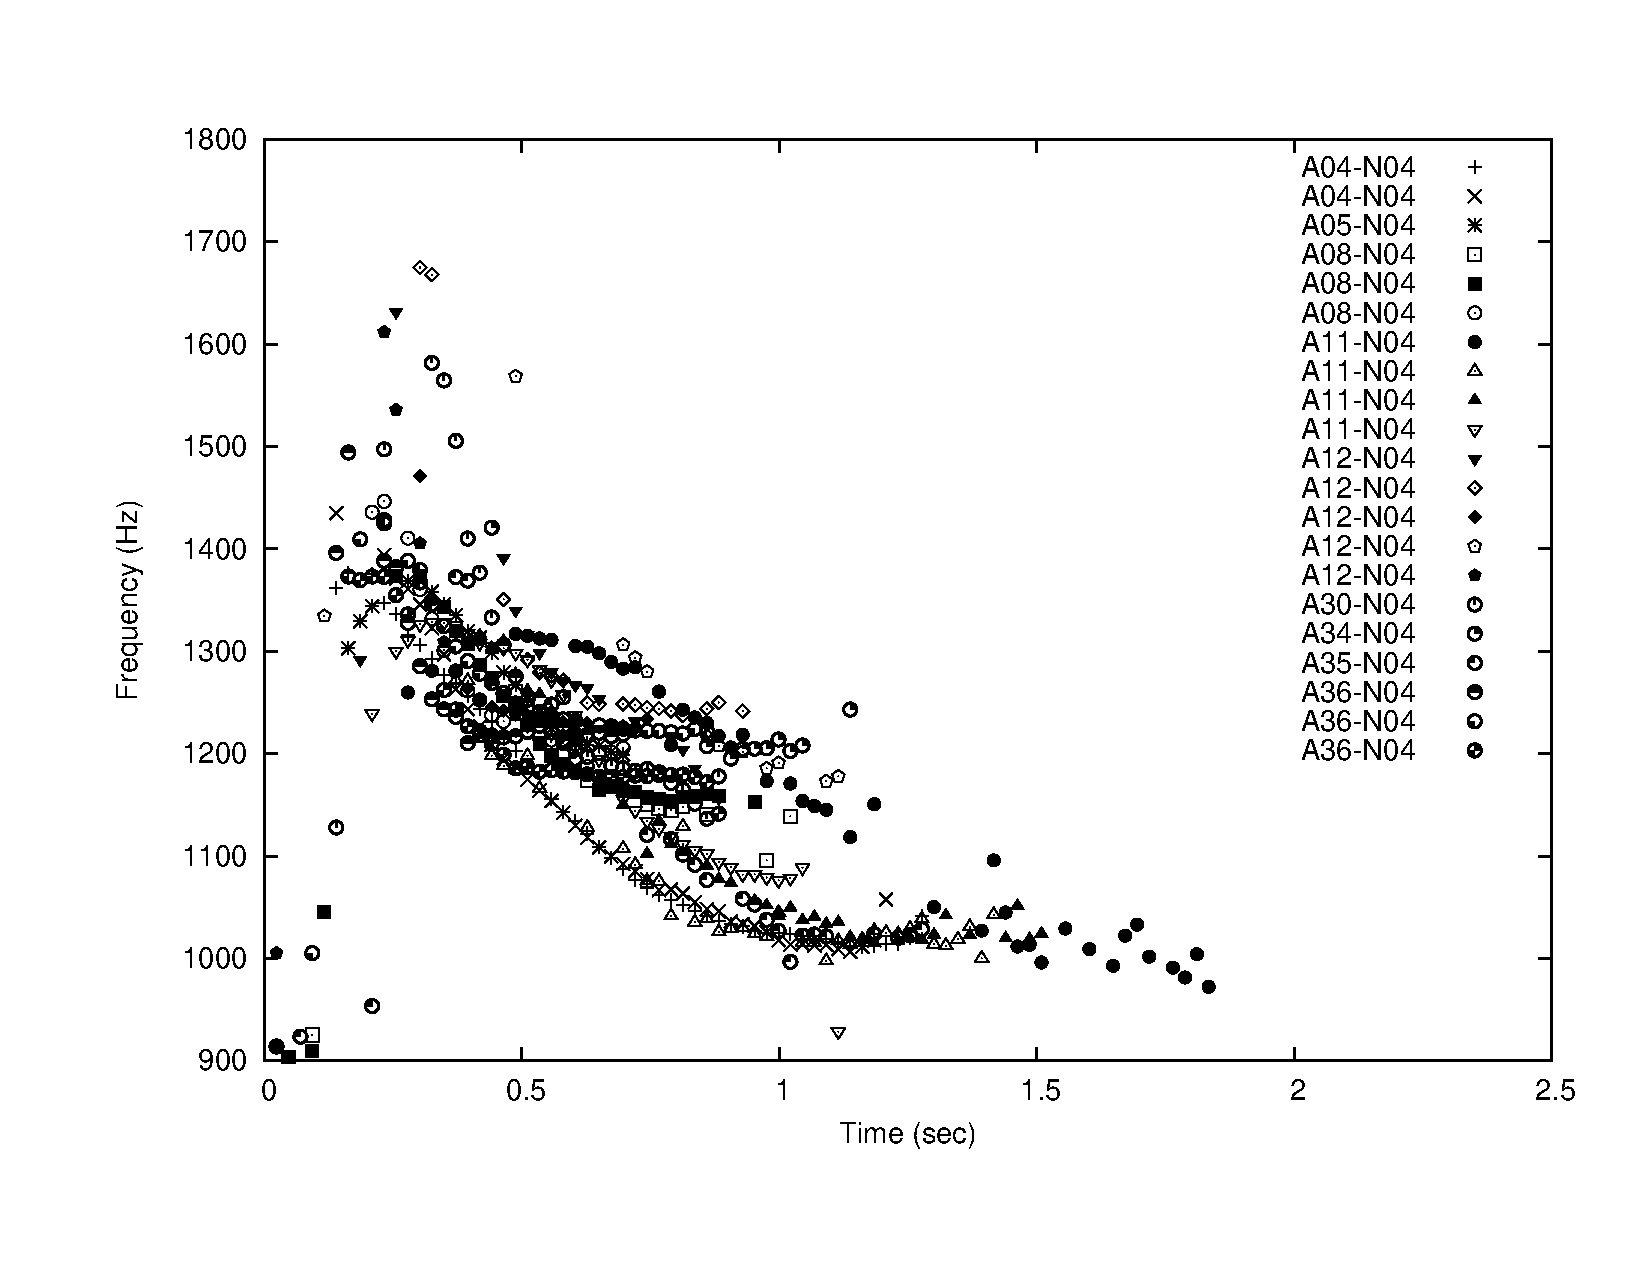
\includegraphics[width=90mm]{figures/pitch-N04}
%% \caption{F0 contour for 21 examples of the N04 call.}
%% \label{fig:pitch-N04}
%% \end{figure}

%% \begin{figure}[h]
%% \centering
%% 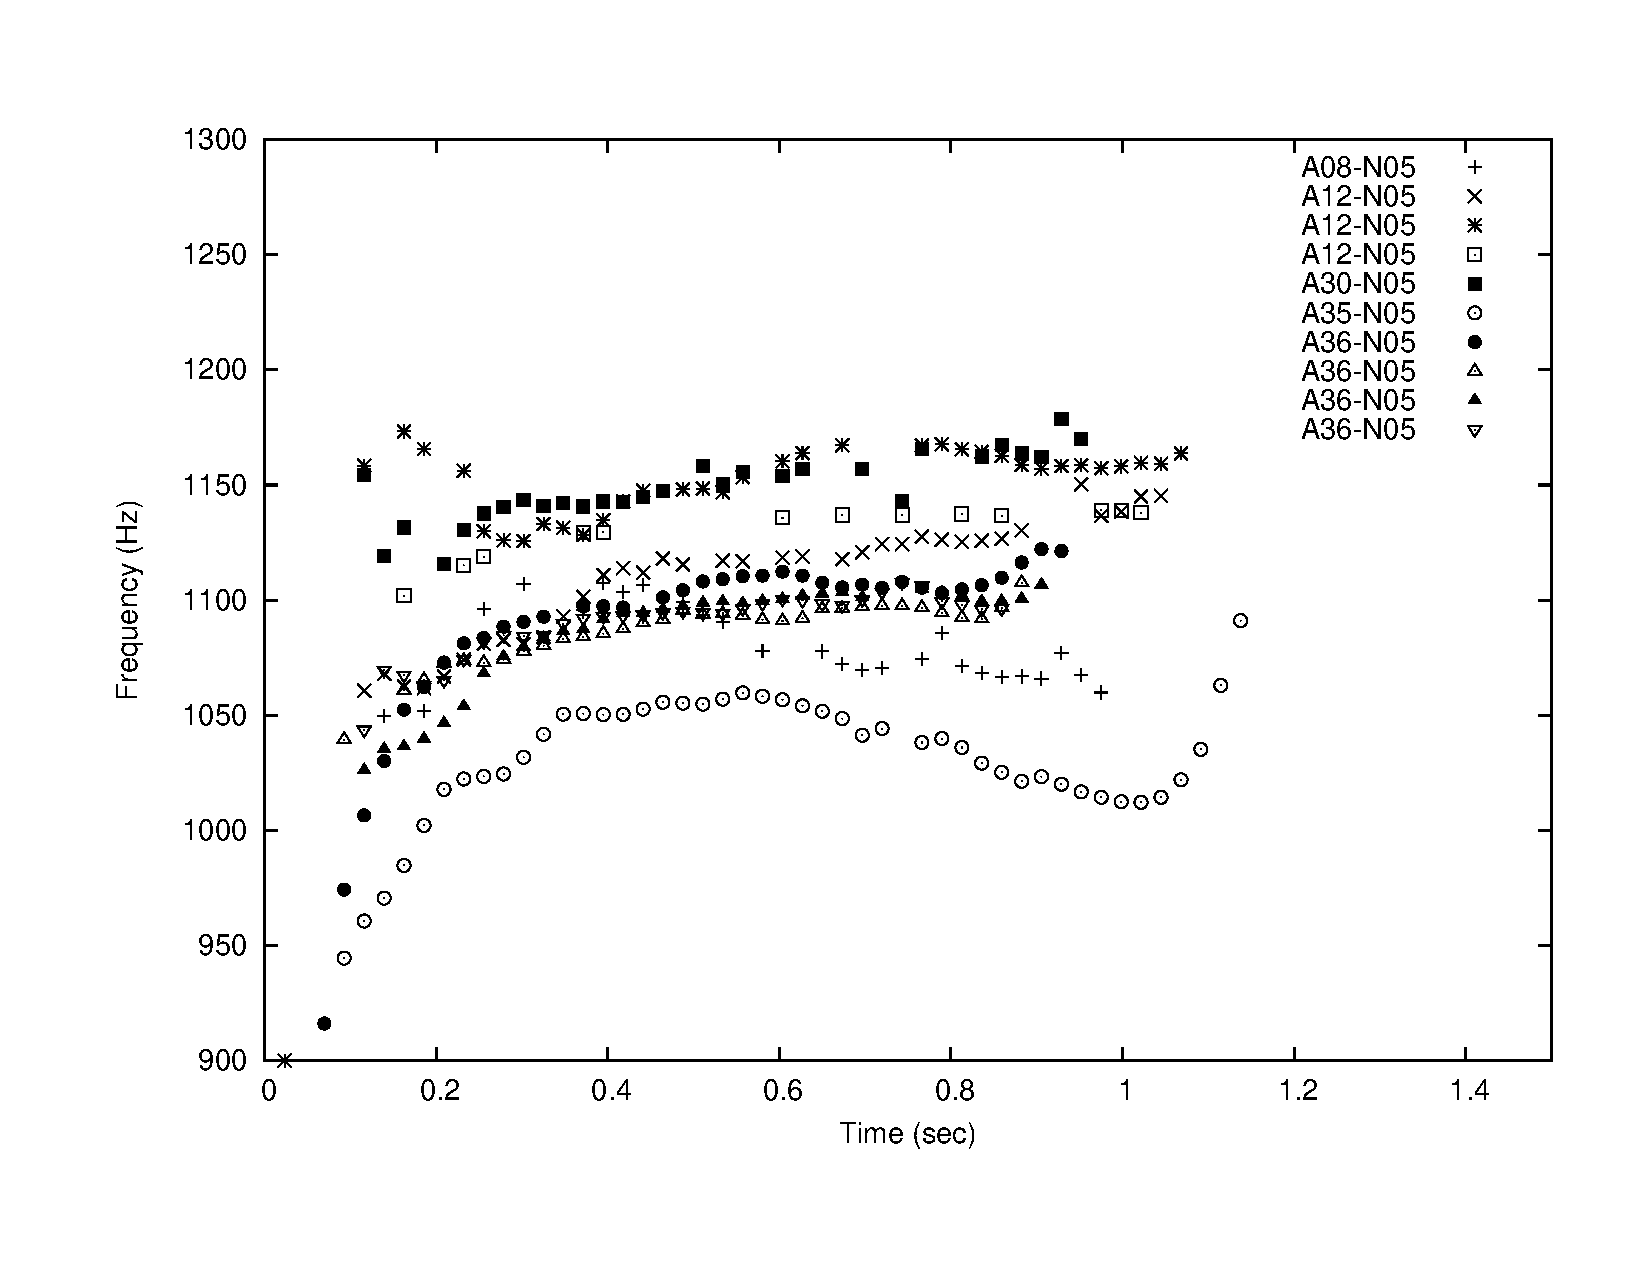
\includegraphics[width=90mm]{figures/pitch-N05}
%% \caption{F0 Contour for 10 examples of N05 call.}
%% \label{fig:pitch-N05}
%% \end{figure}

%% This approach is certainly valid if slope changes within a given
%% window characterize the signal well and the signal is fairly free of
%% noise. We therefore have examined SAX for a possible avenue to
%% transcribe Orca vocalizations. We determined, however, that
%% considering windowed slope fragments of Orca vocalizations does
%% produce sequences that are of lower quality than those produced by our
%% transcription technique which we refer to as FTSQ (Fundamental
%% Frequency Time Series Quantization).  The FTSQ procedure is outlined
%% in detail below. We do not provide classification results for SAX
%% sequences because the majority of SAX sequences were too long in order
%% to be processed by our dynamic programming based alignment algorithm
%% and hence a direct comparison can't be impartial. Further, we observed
%% that the fundamental frequency of Orca vocalizations carries a lot of
%% information, that is, it seems to be stable, and within a certain
%% range that is unique to a large portion of the vocalizations in our call
%% catalog. Since SAX is normalizing the signal slope within a sliding
%% window it cannot take advantage of this important feature.

%% \subsection{Signal Pre-processing and FTSQ}

%% Fundamental Frequency Time Series Quantization is a time series
%% quantization approach that transcribes an audio time series based on
%% an estimate of it's fundamental frequency ($F_0$).

%% In general it is not feasible to analyze Orca vocalizations as a raw
%% time series, since these signals are a complex mixture of sinusoids and
%% noise (see Figure \ref{fig:audio_raw}).  Figure \ref{fig:freqspec}
%% shows a spectrogram representation of the N01 and N09 Orca
%% vocalizations.  When comparing Figures \ref{fig:audio_raw} and
%% \ref{fig:freqspec} it is easy to see that the frequency components of
%% the audio signal reveals much more about the structure of the signal
%% than a raw audio time series by itself.

%% \begin{figure}[h]
%% \centering
%% 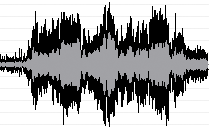
\includegraphics[width=0.4\columnwidth]{figures/audio_raw}
%% \caption{Raw audio signal of Orca vocalization N01.}
%% \label{fig:audio_raw}
%% \end{figure}
%% \begin{figure}[h]
%% \centering
%% 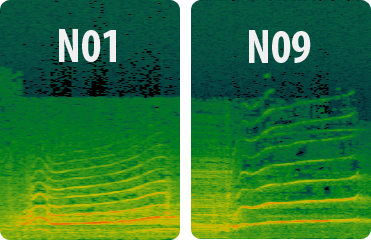
\includegraphics[width=0.60\columnwidth]{figures/freq_N01N09.png}
%% \caption{Frequency spectrum of Orca vocalizations N01 and N09.}
%% \label{fig:freqspec}
%% \end{figure}

%% Quantizing the fundamental frequency of an audio signal is am approach that makes 
%% use of the underlying structure in the frequency bands of the audio signal.
%% Loosely speaking one may think of the fundamental frequency as the pitch of a sound signal.
%% For our FTSQ technique we use Yin \cite{Cheveigne2002} a robust fundamental frequency 
%% estimation algorithm developed by Cheveigne et al.
%% Processing the audio waveform from Figure~\ref{fig:audio_raw} with Yin yields the 
%% fundamental frequency (in octaves relative to 440 Hz) shown in the top plot of Figure \ref{fig:yin}.
%% The two plots below the fundamental frequency show the aperiodicity and the
%% period-smoothed instantaneous power of the signal; they give estimate in the 
%% confidence on the approximation of $F_0$ and are used to identify meaningful
%% regions of interest within the $F_0$ signal.
%% \begin{figure}[h]
%% \centering
%% 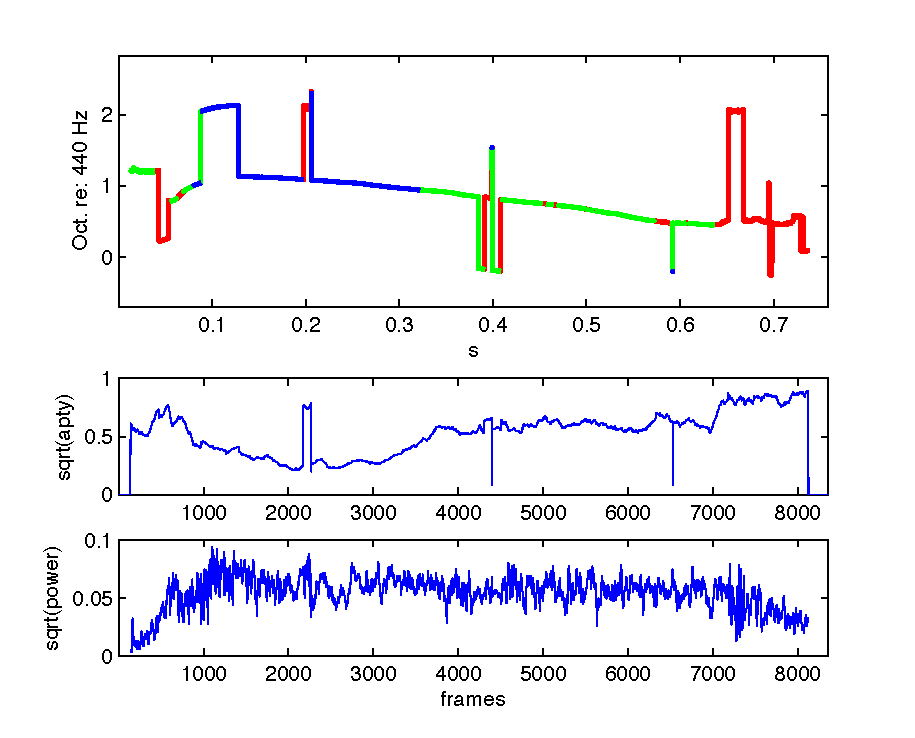
\includegraphics[width=\columnwidth]{figures/yin}
%% \caption{Frequency spectrum of Orca vocalizations N01 and N09}
%% \label{fig:yin}
%% \end{figure}


%% A further issue that is encountered commonly in the process of
%% determining a pitch contour for an audio recording is the optimization
%% of all the parameters of the pitch detection algorithm to perform well
%% on the particular dataset that is being used.  There are many such
%% parameters for each different algorithm, the important ones in the Yin
%% algorithm include the window size and hop size of the FFT, the high
%% and low frequency cutoffs, the high and low frequencies around which
%% the pitches will be wrapped using modulo arithmetic, the tolerance of
%% the Yin algorithm which determines which peaks in the autocorrelation
%% will be used for the pitch determination, the window size for the
%% median filter, and the number of histogram bins in which to divide the
%% frequency range into.  In our previous work, this was done by hand by
%% plotting points using MATLAB or Gnuplot, which can be a long and
%% labour intensive process.

%% For this project, we added custom visualization tools to our OpenMIR
%% platform to view the original audio as a spectrogram, to allow the
%% user to listen to this audio, to show a pitch contour with dynamic
%% controls over these various parameters, and an energy display that
%% shows the RMS energy of the audio signal.  This interface is shown in
%% Figure \ref{fig:openmir}.  This software allowed us to quickly
%% iterate over a large number of parameters, and to determine the
%% optimal parameters for the Yin algorithm.  The most important of these
%% was the median filter size, and a median filter of size 11 is shown in
%% Figure \ref{fig:openmir}.

%% \begin{figure}[t]
%% \centering
%% 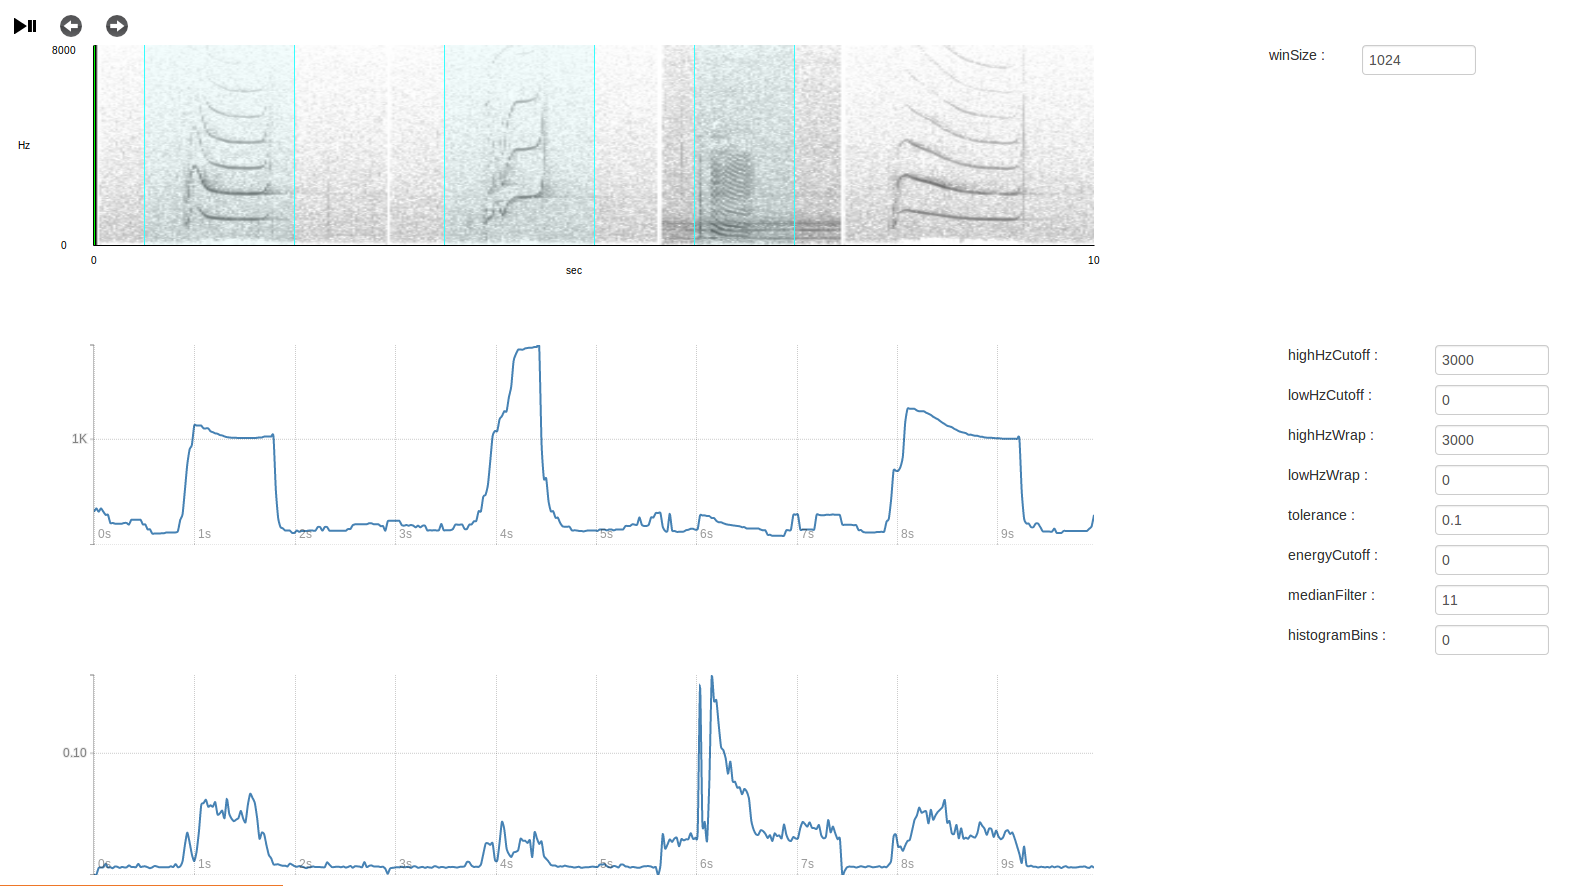
\includegraphics[width=\columnwidth]{figures/openmir}
%% \caption{Spectrogram, pitch and RMS view of a small portion of the Orchive
%% catalog viewed with the OpenMIR interface. }
%% \label{fig:openmir}
%% \end{figure}

%% \subsubsection{Octave Errors}
%% The output of Yin does not always give a proper estimate of $F_0$.
%% Indeed, the $F_0$ signal in Figure \ref{fig:yin} displays several
%% estimation errors that we herein refer to as \emph{octave errors}.
%% Octave errors manifest themselves as sudden jumps in a multiple of the
%% core $F_0$ frequency. Figure \ref{fig:yin} displays multiple octave
%% errors the first one at about 0.1 seconds. When quantizing the $F_0$
%% signal into a letter representation over a finite alphabet. Octave
%% errors result in mis-mapped letters in the output sequence. To a
%% certain degree we are able to handle octave errors by crafting a
%% custom substitution matrix in our sequence alignment
%% algorithm. However, doing so ultimately lowers the confidence in our
%% alignment score and might confuse legitimate frequency jumps with
%% octave errors and as a result would not penalize mismatches
%% appropriately. Therefore, we have developed a technique that can
%% automatically correct for the majority of octave errors and as a net
%% effect produces a more accurate letter representation.

%% We first run the $F_0$ signal obtained from Yin through a median filter, 
%% which smoothes the signal and eliminates small transients that occur due
%% to noise in the original signal. We then threshold the aperiodicity and the
%% period-smoothed instantaneous power to obtain $F_0$ signal regions at which
%% the $F_0$ signal is estimated with high confidence. After down-sampling the
%% signal we obtain the representation shown in Figure
%% \ref{fig:clean_yin}.

%% \begin{figure}[h]
%% \centering
%% 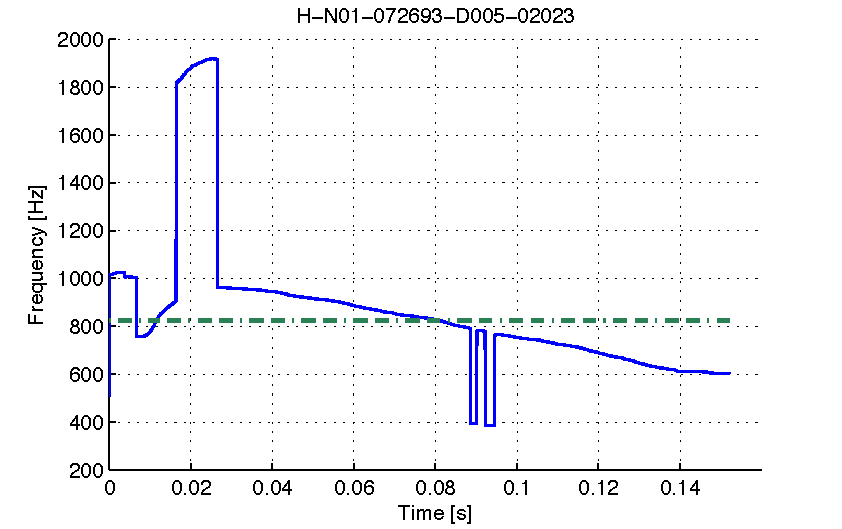
\includegraphics[width=\columnwidth]{figures/yin_clean}
%% \caption{Thresholded and down-sampled $F_0$ signal of a N01 call.}
%% \label{fig:clean_yin}
%% \end{figure}

%% The green line represents the median of the original $F_0$ signal
%% drawn in blue. The octave errors are clearly identifiable as such in
%% Figure \ref{fig:octave_yin} which shows versions of the $F_0$ signal
%% one octave above (purple) and on octave below (red) the original
%% (blue).  $F_0$ signal. To correct for octave errors we simply piece
%% the portions of the three versions of the $F_0$ signal together
%% according to which ever signal is closest to a slightly upwards biased
%% median of the original signal (blue). This yields the black $F_0$
%% curve wich shows the now automatically corrected version of the $F_0$
%% signal.
%% \begin{figure}[h]
%% \centering
%% 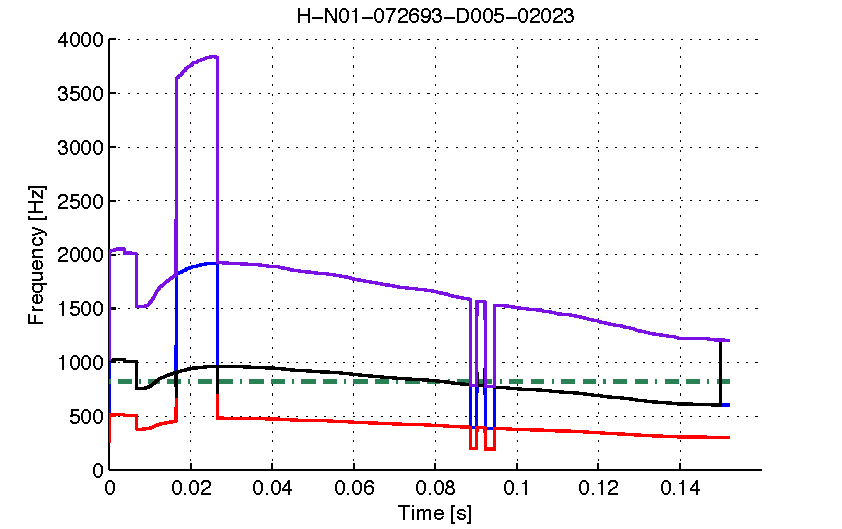
\includegraphics[width=\columnwidth]{figures/octave_fix}
%% \caption{Octave errors within a $F_0$ signal of a N01 call.}
%% \label{fig:octave_yin}
%% \end{figure}

%% \subsection{Log-Normal Signal Quantization}
%% When transcribing the $F_0$ signal into a letter representation suitable 
%% for sequence alignment tools it is natural to ask how these letters should be
%% assigned over the range of possible $F_0$ frequency values. A naive approach
%% would be to map $F_0$ frequencies to letters in a linear fashion. However, while
%% this approach does work well in practice, we investigated if a non-linear mapping
%% might potentially be more appropriate. For this purpose we plotted
%% the distribution of $F_0$ frequencies over time for the whole catalog of
%% Orca vocalizations in Figure \ref{fig:freq_dist}. The dynamic range of
%% $F_0$ incorporates frequencies from about 80 to 2400Hz, with three high density bands
%% at around 250, 700 and 1200Hz. Ideally one would therefore quantize the $F_0$ signal
%% using a three-modal distribution. However, for simplicity we chose a log-normal 
%% distribution (see Figure \ref{fig:log_norm}), which provides us with a fine resolution
%% for the more common $F_0$ frequencies and quantizes high $F_0$ frequencies at a coarser level.
%% \begin{figure}[h]
%% \centering
%% 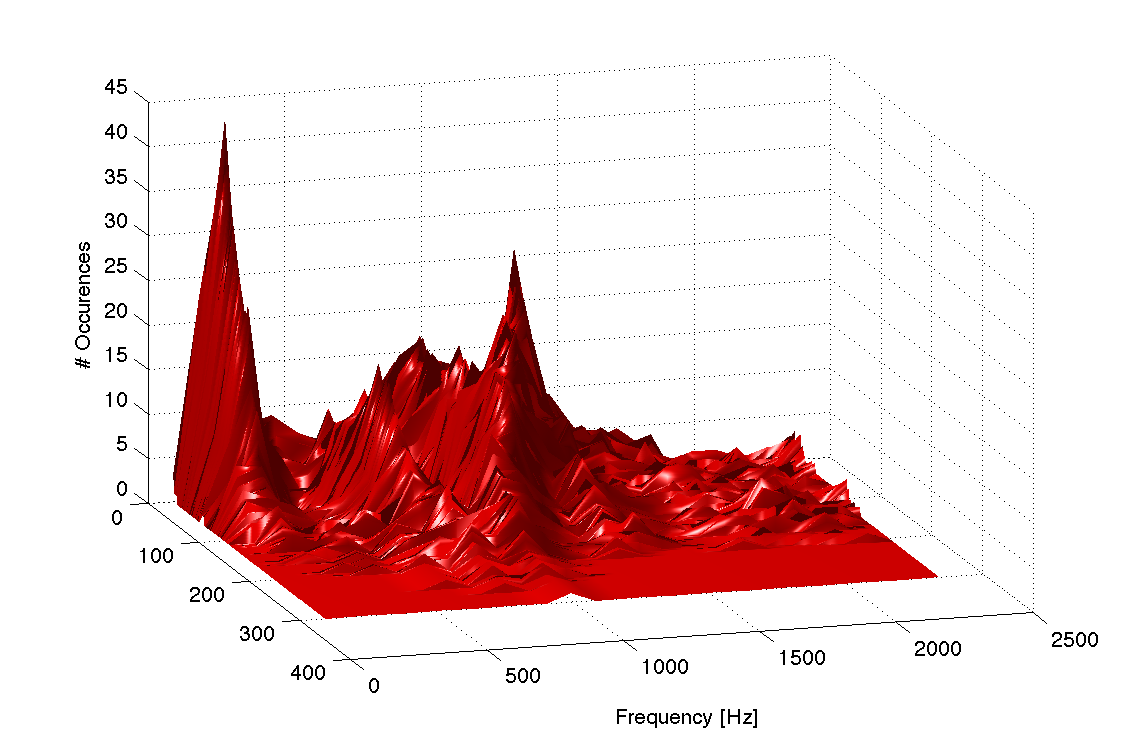
\includegraphics[width=\columnwidth]{figures/freq_dist}
%% \caption{Distribution of $F_0$ frequencies of call catalog.}
%% \label{fig:freq_dist}
%% \end{figure}

%% \begin{figure}[h]
%% \centering
%% 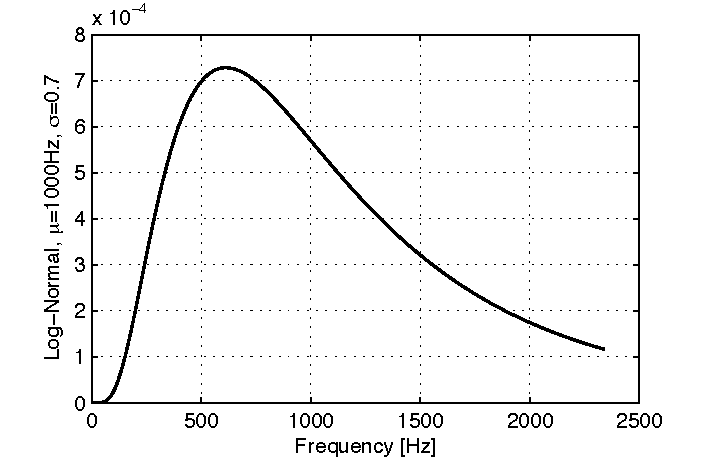
\includegraphics[width=0.7\columnwidth]{figures/log_norm}
%% \caption{Log-normal distribution for quantization}
%% \label{fig:log_norm}
%% \end{figure}

%% The result of log-normal quantization of the $F_0$ trace in Figure
%% \ref{fig:octave_yin} is provided in Figure
%% \ref{fig:letter_curve}. Finally, the resulting letter sequence is
%% given by \texttt{LLHHJJKKKKKKKKKKKKJJJJJJJII--IIIIIHHHHHHHGGGGGFFFFFF}
%% which can readily be consumed by a dynamic programming sequence
%% alignment algorithm.

%% \begin{figure}[h]
%% \centering
%% 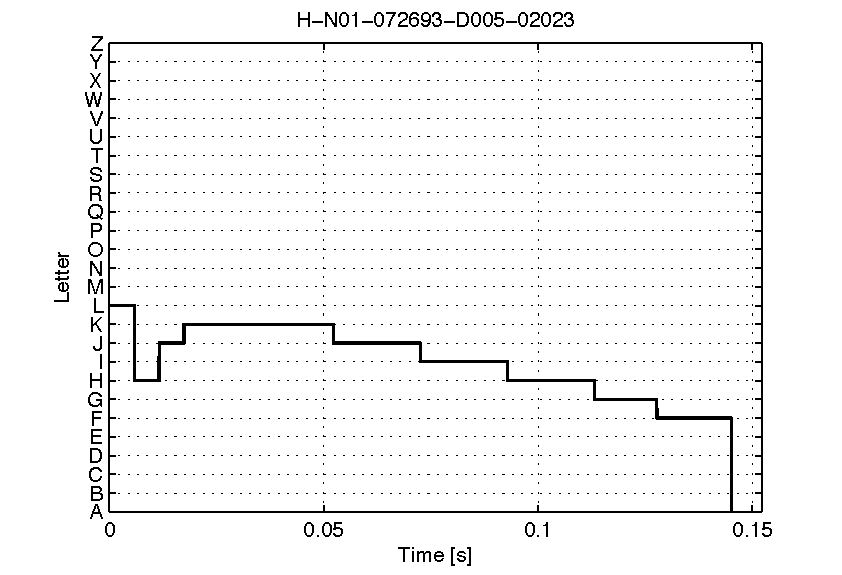
\includegraphics[width=\columnwidth]{figures/letter_curve}
%% \caption{$F_0$ signal of N01 call quantized to a finite alphabet}
%% \label{fig:letter_curve}
%% \end{figure}

%% \begin{table}
%% \centering
%% \begin{tabular}{|c|c|} 
%% \hline
%% Data Set                         &  Global Accuracy  \\
%% \hline
%% Original                         &              64\%  \\
%% Octave Removal - Linear          &              81\%  \\
%% Octave Removal - NonLinear 900   &              80\%  \\
%% Octave Removal - NonLinear 1200  &              81\%  \\
%% J48                              &              58\%  \\
%% Naive Bayes                      &              65\%  \\
%% SVM                              &              75\%  \\
%% \hline
%% \end{tabular}
%% \caption{Global accuracy for different methods of converting a Yin
%%   pitch contour into an alphabet using FTSQ}
%% \label{table:performance}
%% \end{table}


%% \begin{table}
%% \centering
%% \begin{tabular}{|c|c|} 
%% \hline
%%  Call  &  Accuracy  \\
%% \hline
%%  N47   &     0.400  \\
%%  N01   &     0.969  \\
%%  N12   &     0.583  \\
%%  N05   &     0.785  \\
%%  N04   &     1.000  \\
%%  N03   &      0.75  \\
%%  N09   &     0.772  \\
%% \hline
%% \end{tabular}
%% \caption{Global accuracy for different call types using Octave Removal
%%   NonLinear 1200 parameters with the FTSQ algorithm.}
%% \label{table:performance}
%% \end{table}

%% \section{Alphabetic Sequence Representation}

%% In order for sequence comparison algorithms to work well, it is
%% necessary that the combination of the letters and the scoring matrix
%% are compatible and output meaningful results.  In the two sections
%% below, we show the result of quantizing the signal using the nonlinear
%% histogram approach for two of the more common calls vocalized by
%% A-clan Northern Resident whales.  The first is the very common N4
%% call, which consists of a quick up swing in pitch, followed by a
%% downswing and then a constant tone.  In it we can clearly see long
%% regions of the repeated letters, P,O,N,M,L,K.  Even from a quick
%% visual inspection these repeated letters show that our method of
%% converting frequencies into a discrete alphabet is promising.

%% {\tiny
%% \begin{verbatim}
%% N04 A04 HIKNOOOOOPPPPOOOOOOOOOOOONNNNNNNNNNNNMMMMMMMMMMMMLLLLLLLLLLLLLLLLLLKKKKKKKKKKKKKKK
%% N04 A04 IJNOPPPPPPPPPPPOOOOOOOOONNNNNNNNMMMMMMMMMMMMMMLLLLLLLLLLLLLLLLLLLLLLKKKKKKKKKKKKKK
%% N04 A05 NLKLMNOOOOOOOOOOOOOOOOOOOOOOOOOONNNNNNNNNNNNNNNNNNNNMHGQ
%% N04 A08 RILMNNOOOOOOOOIIOOOOOOOOOOONNNNNNNNNNNNNNNNNNNNNMMMMMMMMMMMMMMMMMMMMMLLLLLLLMLLLLL
%% N04 A08 SIIJJKNPQQRPIIOOOOOOOONNNNNNNNNNNNNNMMMMMMMMMMMMMMMMMMMMMMMMMMDCCCMMM
%% \end{verbatim}
%% }

%% Even more promising were the results for another call, N5, which
%% consists of a constant tone.  These calls are from the A36 matriline
%% of orcas, which now consists of only two whales, the brothers A37 and
%% A46, although the grandmother whale, A12 often now associates with
%% this matriline after A34, her daughter's matriline, grew large in
%% size.  From these calls, we can see that the frequency represented by
%% the letter L is very constant throughout the entire call, and is a
%% clear indication that this is an N5 call.

%% {\tiny
%% \begin{verbatim}
%% N05,A36,A36-N05-070806-D012-13913,IIJJJKKKKKLLLLLLLLLLLLLLLLLLLLLLLLLLLLLLLLLLLLLLLLLLLLLL
%% N05,A36,A36-N05-070806-D012-13917,JJJKKLLFLLLLLLLLLLLLLLLLLLLLLLLLLLLLLLLLLLLLLLLLLLLLLLLL
%% N05,A36,A36-N05-070806-D012-13921,IIJJKKKKKKKKKLLLLLLLLLLLLGLLLLLLLLLLLLLLLLLLLLLLLLLLLLLL
%% N05,A36,A36-N05-071506-D017-11311,IQHJKLLLLLLLLLLLLLLLLLLLLLLLLLLLLLLLLLLLLLLLLLLLLLLLLLLL
%% \end{verbatim}
%% }


%% Praat \cite{boersma93} is another modern pitch determination
%% algorithm, it is an autocorrelation based approach that provides good
%% robustness by making the assumption that pitch is stable in a small
%% window.  It uses a Hanning or Gaussian window to smooth the edges of
%% the window to be analyzed and finds peaks that occur after the zero
%% lag peak.  It has been shown to work well for estimatating the pitch
%% of human speech signals.


%% We have compared three pitch extraction methods for obtaining the
%% pulse rate contour. The first method ({\bf PRAAT}) is based on
%% time-domain autocorrelation and is similar to the pitch extraction
%% algorithm implemented in Praat \cite{boersma93}. It is based on
%% calculating the time-domain autocorrelation of the signal:

%% \begin{equation} 
%% R(\tau) = \frac{1}{N} \sum_{n=0}^{N-1-m} x[n] x[n+m] \;\;\;\; 0 \leq m
%% < M 
%% \end{equation} 

%% The peaks of the autocorrelation function correspond to the lags 
%% in which the signal is self-similar. The signal is processed in
%% windows and the autocorrelation of the windowed signal $R_{xw}$ is divided 
%% by the autocorrelation of the window $R_{w}$ providing better robustness to 
%% noise and better accuracy. 

%% \begin{equation}
%% R_{x}(\tau) = R_{xw}(\tau) / R_{w}(\tau)
%% \end{equation} 


%% %
%% % Deep Belief Network
%% %

%% \subsection{Deep Belief Network}


%% - description of Deep Belief Networks

%% \begin{table}
%% \begin{tabular}{|l|l|l|l|l|}
%% \hline
%% Window Size & Hop Size & Memory & Total feature vectors & Percent Correct \\
%% \hline


%% \hline
%% \end{tabular}
%% \caption{Table of downsampling 100 (or whatever is reasonable) with weka with
%% MFCC + Spectral with different}
%% \label{table:mfccSpectralWeka}
%% \end{table}



%% Mahout is an excellent system, with many powerful capabilities and
%% with deep integration into Hadoop.  In our tests, we found the most
%% difficult thing as a student was to get the resources to run a
%% reasonably large (10-20 node) Hadoop cluster.  As we described in the
%% report, it is no small feat to get the Hadoop cluster installed and
%% running, especially on unknown hardware, but once this is done, Mahout
%% is simple to use and allows the storage of results on HDFS, the use of
%% which is almost essential, given the quantity of final and
%% intermediate results that need to be stored for a typical experimental
%% setup.  

%% Ethnomusicology (Musicology) - a sub-discipline of Musicology that
%% focuses on the study of the socio-cultural aspects of music in
%% societies around the world.  \\

%% Folksonomy (Computer Science) - a system of classification that comes from a group of users collaboratively creating and managing tags in an effort to annotate and categorize content
%% \\

%% Ontology (Computer Science) - a formal representation of ideas or
%% concepts and the relation between them.  This Computer Science
%% definition of ontology is a subset of the broader philosophical idea
%% of ontology, which is a study of what exists and what can exist.  \\

%% Syrinx - One of the structures in birds that is used to produce sound

%% Cantillion : \url{http://cantillion.sness.net}.
%% \\

%% Audioscapes : \url{http://audioscapes.sness.net}
%% \\

%% Dynamic time warping (DTW) is a technique for measuring the similarity
%% of two sequence that many vary in time. It mostly known in the context
%% of speech recognition \cite{sakoe78} but it has found applications in
%% many areas including video, motion and DNA sequence analysis. The use
%% of DTW to compute the similarity between two pulse rate contours in
%% the context of Orca calls has been explored in
%% \cite{brown07_orca_dtw}. In that work, a similarity matrix is
%% calculated containing all the DTW alignment costs between pairs of
%% pulse rate contours. This similarity matrix is then subsequently used
%% to calculate clusters which are then compared the ground truth call
%% labeling to assess the feasibility of call classification using this
%% approach.



%% \section{Introduction}\label{sec:introduction}

%% There are a number of large bioacoustic archives that have been
%% described in the literature, and as computer storage grows ever
%% larger, more of these archives are being created.  In this work, we
%% will focus on two such large bioacoustic datasets, The Orchive, and
%% the recordings made by the Alberta Biodiversity Monitoring Institute
%% (ABMI).  The Orchive is an archive of sounds collected by a network of
%% stationary, permanently mounted hydrophones, and the primary sound
%% that was of interest to the researchers was that of Orcas.  The ABMI
%% dataset is collected at a series of 1700 sites in Alberta using
%% a specialized stereo microphone device.

%% While these two datasets on the surface would appear to be very
%% different, the underlying data collected by both is audio, and the
%% tools to study both these sources of data are in large part very
%% similar.  These tools include a web-based interface to allow
%% researchers to listen to, view and annotate this audio, tools to
%% extract and view audio features from this data, and tools to run
%% machine learning software and view the results of this analysis.


%% The approach of Symbolic Aggregate Approximation (SAX) is one such
%% approach, and we will examine the use of these types of algorithms to
%% the study of large collections of data.


%% In addition, in many cases, because of the large amount of data
%% traditional algorithms cannot be used to analyze this data.  For
%% example, one algorithm used traditionally in analyzing audio is the
%% Dynamic Time Warping algorithm.  In a naive implementation, this
%% algorithm requires $O(n^2)$ time and space complexity, when run on
%% small datasets, this is acceptable, but is not when run on datasets
%% of many thousands of hours.  In many cases, the we must search for
%% linear ($O(n)$) algorithms in order to make the problem tractable,
%% however, algorithms that exhibit constant time performance ($O(1)$)
%% would be even more preferable.

%% In order to study these complex and oft-time messy datasets, one
%% must use a hybrid approach that combines tools that allow for
%% exploration of datasets to allow for the formation of hypotheses.


%% 7) Transformation of audio features into string based representations,
%% and the use of tools from bioinformatics to search through these
%% datasets, and the results showing the benefits of using these
%% algorithms on bioacoustic data.


%% Although this project concentrated on classification, it is the
%% clustering capabilities of Mahout that would be useful for this task,
%% and would be even more appropriate for doing large scale clustering
%% than for doing classification.

%% We will then examine the use Machine Hearing algorithms based on
%% models of the human peripheral auditory system, these algorithms
%% typically first use a filterbank to model the function of the
%% cochlea, followed by a strobed temporal detection system to model
%% the medial superior olive brain center, which provides an
%% autocorrelation-like output for each channel of the filterbank.  We
%% will review literature on the use of the output of this system, the
%% correllogram, and it's use for the recognition of sounds.


%% In humans sounds pass through the ear canal and impact on the ear
%% drum, which is connected to three small bones, terminating in the
%% stapes (stirrup) which is connected to the oval window of the cochlea.
%% The cochlea is a fluid-filled spiral shaped organ which contains a
%% variety of structures, including the scala vestibuli, the scala
%% tympani and the basilar membrane.  The vibrations transmitted to the
%% oval window travel through the scala vestibuli and different
%% frequencies crest at different locations on the basilar membrane.
%% These vibrations move small cilia which are connected to nerves that
%% send electric impulses to the Medial Superior Olive, a nexus of
%% neurons that performs a peak triggering function similar to
%% autocorrelation \cite{lyon10}.  This means that the human hearing
%% system is sensitive to different frequencies, but is also sensitive to
%% the fine-timing relations of peaks in the waveform in the different
%% freqency bands correpsonding to place along the basilar membrane.
%% \cite{waltersphd}.

%% - Importance of not including background noise in the classification
%% - Initial clips from expert users had quite a bit of silence before and after.
%% - Tested to see how this affected the results

%% \begin{table}
%% \begin{tabular}{|l|c|l|l|r|r|}
%% \hline
%% Training       & length  & \% corr.     \\
%% dataset        &  (sec)  &  10-fold     \\
%% \hline
%% non trimmed    &         &              \\
%% hand trimmed   &         &              \\
%% \hline
%% \end{tabular}
%% \caption{Classification results with hand trimmed orca vocalizations
%%   using bextract using an SMO SVM classifier.}
%% \label{table:handTrimmed}
%% \end{table}

%% From these results, it was determined that it was important to trim
%% the clips from the experts into clips that just contained orca calls.
%% This process was done by concatenating all the xxxxx clips labelled
%% orca into one recording and then to use the new expert interface to
%% make clips of just the orca vocalizations with no background.  This
%% resulted in xxxx clips of orca vocalizations.

%% A similar procedure was used for the background clips to ensure the
%% clips labelled background contained no orca vocalizations.  From this
%% it was found that only a very small fraction of the clips labelled
%% background were misclassified by the experts (3 such clips were found
%% out of xxxx total).

%% To obtain clips containing only voice notes, xxxx voice clips were
%% joined together and Audacity \cite{audacity} was used to remove all
%% small sections of silence from this recording.  When these voice notes
%% were recorded by OrcaLab, they were recorded onto only one channel of
%% the tape, typically the right channel.  This makes the identification
%% of voice clips substantially easier for a machine learning system than
%% finding clips containing orca, so this small set of data for voice
%% over was considered to be sufficient.  In addition, the primary goal
%% of the current to find clips containing orca vocalizations, so the
%% exact labelling of voice regions was considered to be of lesser
%% importance.  However, visual inspection of a substantial number of
%% recordings shows that good precision and recall of voice notes was
%% also found.



%% %
%% % Spectrogram image
%% %

%% Spectrogram image



%% \begin{table}
%% \begin{tabular}{|l|l|l|l|l|}
%% \hline


%% \hline
%% \end{tabular}
%% \caption{}
%% \label{table:obv-5-spectrogramImage}
%% \end{table}




%% In this paper, we will examine the combination of three components of
%% distributed cognition to help work on the problem of analyzing orca
%% vocalizations:

%% - Collaborative technologies to enable distributed cognition between
%% expert users in with potentially diverse domain knowledge

%% - The use of machine learning algorithms to provide technologies for
%% Intelligence Augmentation

%% - The use of large numbers of people from the general public in a
%% crowdsourcing methodology to mine through and annotate large databases
%% of information

%%   One approach to classifying sounds is the use of Dynamic Time
%% Warping, an approach used in the analysis of human speech, and
%% which has had success in the study of biacoustics.


%% A literature review of papers on the use of machine learning
%% algorithms on the output of audio feature extraction algorithms to
%% analyze sound will then be presented.  Although this is a relatively
%% new field of study, the literature on this subject is vast, and the
%% primary focus will be on the use of machine learning algorithms in the
%% study of bioacoustics.  This is distinct from the study of music and
%% other forms of audio using these same algorithms.  We will briefly
%% examine the use of older methods such as tree building algorithms and
%% multilayer perceptrons as well other machine learning algorithms.  

%% will then focus our attention on the use of Support Vector Machines
%% for audio classification.


%% Their system has a Master Node computer that coordinates all tasks,
%% Library Nodes that coordinate tasks for a single library and Worker
%% Nodes that perform feature extraction.  In their system, Library Nodes
%% store the raw data and distribute it to the Worker Nodes.  One
%% possible sub-optimal case would be if a single Library Node got
%% overwhelmed with requests, in this case, it would be challenging to
%% get other Library Nodes to serve requests to new Worker Nodes.



%% We explore three retrieval strategies/representations. Statistical
%% features characterizing the entire pulse rate contour are computed and
%% each call is characterized by a single vector of features. The
%% features are normalized by max-min normalization so that they range
%% from 0 to 1 over the entire dataset. Similarities are then computed by
%% taking the Euclidean distance in the normalized space. This strategy
%% is used as reasonable baseline. The features used in this work are the
%% mean, median, standard deviation, min and max of the pulse rate
%% contour. The second strategy consists of resampling the pulse rate
%% contour using linear interpolation to a fixed number of points. This
%% strategy is similar to the one used in Deecke
%% \cite{deecke99_quantifying_orca}. Essentially it assumes that the
%% duration of the call does not play a major role in its
%% characterization and temporal scaling is applied uniformly across the
%% contour. The third strategy utilizes dynamic time warping to align the
%% pulse rate contours. The alignment cost is used to measure the
%% similarity between calls. The two sequences to be matched are arranged
%% on the sides of a grid. To find the best match between the sequences
%% we can find a path through the grid that minimizes the total distance
%% between them. More details can be found in \cite{sakoe78}.

%% Another modern pitch detectors that we used in previous work is the
%% SWIPEP \cite{camachophd} algorithm which determines clusters of
%% pitched and unpitched sounds.  This algorithm was less appropriate to
%% use on the mostly pitched discrete calls that orcas produce, but could
%% be of benefit when studying bird calls that contain both pitched and
%% unpitched regions.


%% Dolphins (and presumably orcas) have about the same number
%% of inner hair cells but have 3 times as many gangilon cells.  (How
%% would this affect things?)

%% - We then did a test to see if adding other features helped the
%% classification using the window size, hop size and memory from the
%% last experiment.
%% - We added spectral features including Centroid, Rolloff, and Flux
%% - Description of Centroid, Rolloff, Flux, Kurtosis
%% - Added Linear Prediction Coefficients
%% - LPCC - Convert LPC coefficients to Cepstrum coefficients.
%% - LSP - Linear Spectral Pair
%% - Spectral Crest Factor
%% - Spectral Flatness Measure 
%% - Zero crossings
%% - Added pitch detector - Yin
%% - Added Chroma


%% Another algorithm that is useful for studying sounds with multiple
%% pitches is the SACF algorithm of Tolonen and Karjalainen
%% \cite{tolonen00}.  In this algorithm, the signal is decomposed into
%% two frequency bands (below and above 1000 Hz) and amplitude envelopes
%% are extracted for each frequency band. The envelope extraction is
%% performed by applying half-wave rectification and low-pass filtering.
%% The envelopes are summed and an enhanced autocorrelation function is
%% computed so that the effect of integer multiples of the peak
%% frequencies to multiple pitch detection is reduced.

%% One widely used method is based on the {\bf YIN} pitch extraction
%% method.  The YIN method is based on the difference function which is
%% similar to the autocorrelation:

%% \begin{equation}
%% d{t} = \sum_{n=0}^{N-1} (x[n] - x[n+\tau])^{2}
%% \end{equation} 

%% The dips in the difference function correspond to periodicities. 
%% In order to reduce the occurrence of subharmonic errors, YIN employs a
%% cumulative mean function which de-emphasizes higher period dips 
%% in the difference function. 

%% The third method ({\bf SACF}) is based on the multipitch detection
%% algorithm described by Tolonen and Karjalainen \cite{tolonen00}.  In
%% this algorithm, the signal is decomposed into two frequency bands
%% (below and above 1000 Hz) and amplitude envelopes are extracted for
%% each frequency band. The envelope extraction is performed by applying
%% half-wave rectification and low-pass filtering.  The envelopes are
%% summed and an enhanced autocorrelation function is computed so that
%% the effect of integer multiples of the peak frequencies to multiple
%% pitch detection is reduced.

%% The discrete calls of killer whales are pulsed signals in which a tone
%% (of a certain tonal frequency) is not emitted continuously but in
%% pulses given by the pulse-repetition rate. Unlike the tonal signals of
%% many birds and other delphinids, the highest energy is not always
%% contained in the first or second harmonic
%% \cite{deecke99_quantifying_orca}. The high levels of background noise
%% and variety of recording conditions compound the difficulty of
%% obtaining pulse rate contours. The pulse rate contour is used as the
%% primary representation for Orca calls because it is more robust as
%% compared to spectral features to levels of background noise typical in
%% field recordings.



%% The Music Information Retrieval tools used to analyze this audio are
%% also impractical to use on a single computer, the time it takes to
%% analyze the audio, and the amount of storage space makes it
%% impractical to analyze large collections of audio data on a single
%% computer.  


%% DTW is used frequently in the field of MIR, and this thesis
%% discusses its use as applied to chant traditions from cultures
%% around the world in Appendix B.


%% \section{Web based interfaces}


%% - Expert Interface
%% - Citizen Science Interface
%% - Old interface
%% 	- Static resources
%% 	- Difficult to regenerate
%% 	- Many different technologies
%% 		- RoR, HaXe, Flash, Javascript, Python, C++
%% 	- Files generated by hand and manually added to server
%% 	- Many different websites with different technology


%% - New interface
%% 	- Fewer technologies
%% 		- Javascript (client+server), Python, C++
%% 	- Unified interface to all technologies
	%% - Interfaces to many programs

%% This game was designed to be the simplest possible game like interface
%% that would gather data for this project.  Last year, we had written a
%% much more involved interface that had many more features, such as
%% multiple turns per level where the user was first presented with only
%% the sounds and was asked to guess the clip, then if they got it wrong
%% they were allowed to see the spectrogram for a brief period of time
%% and guess again, and finally were allowed to see the spectrogram.
%% This interface also had a running score counter, where the user would
%% get points for correct answers, and if they answered correctly with
%% fewer hints in a level, they were rewarded with a higher score.  This
%% interface also had ``achievements'' which were an in game reward given
%% for correctly identifying 10 calls of a specific type, for example the
%% ``N01'' call.  Another form of reward given was that after a series of
%% levels were completed, the user was given a screen showing them some
%% information about orcas along with pictures of orcas.  We hope to add
%% these additional features back into the game at some point, but were
%% interested in the current work if the simplest possible game mechanic
%% was engaging for users.


%%  In future work, we
%% would like to try to use MFCC or other forms of spectral data as input
%% to our symbolic approximation algorithm.


%% An important aspect in the design of a tool to support collaborative
%% work is to consider what user communities will use the tool.  In the
%% case of the Orchive, there are a number of different scientific
%% communities that will be using this tool and the data this tool
%% provides access to.  The primary scientific community that will
%% benefit from this work will be cetacean biologists.  In order to study
%% the rich archive orca vocalizations that have been recorded by
%% OrcaLab, researchers must currently travel to Hanson Island, search
%% through the lab books and incidence reports to find which recordings
%% contain the data they are interested in, locate the physical cassette
%% tape corresponding to this recording, and then either manually listen
%% to the tape, or perhaps digitize the tape and analyze it in the
%% computer.  Each researcher typically then keeps the annotations and
%% data generated from this procedure themselves, if future researchers
%% want to obtain this data for further analysis, they must first be
%% aware of the fact that this researcher has the data, and then request
%% it from them.  With the distributed collaborative system we have
%% designed, not only can these biologists easily listen to any recording
%% in the entire archive from any internet connected computer in the
%% world, and compare different recordings, they can also add their
%% annotations to the system.  These annotations can be either private or
%% public, if they are for use in a publication, after the article has
%% been accepted for publication, the researcher can make their private
%% annotations public.  These researchers are less interested in the
%% details of audio feature extraction and machine learning algorithms,
%% and are instead more focused on asking biologically informed
%% questions, like dialect change in cetacean call repertoire
%% \cite{deecke2000dialect}.

%% Another scientific community that will receive benefits from this
%% archive are the developers of bioacoustic algorithms.  These
%% scientists are typically computer scientists with interests in Music
%% Information Retrieval and bioacoustics.  This archive represents a
%% site where researchers can get large amounts of high quality and
%% uniformly collected data.  Researchers interested in bioacoustic
%% algorithms have different goals and skill sets from cetacean
%% biologists, for example, many have extensive knowledge of Digital
%% Signal Processing and audio feature extraction algorithms.  This
%% system should be flexible and powerful enough to allow these
%% researchers to ask questions that are relevant to them.  The required
%% features for this group of users include allowing them to choose
%% different audio feature extraction algorithms, and to then take the
%% resulting data and run it against a variety of machine learning
%% algorithms in as flexible a manner as possible.

%% \section{Symbolic Approximation of Pitch Contours}

%% There is considerable evidence that individual orca pulsed calls can
%% be divided into different sections, and in fact the main call catalog
%% of the Northern Resident Killer Whales \cite{ford1989acoustic}
%% classifies calls by looking at the properties of different sections of
%% the audio.  If an orca call could be thought of as a word, these
%% sections would be the letters of the word, or a string in the language
%% of computer science.  In recent years, there have been exciting
%% developments in algorithms for searching strings, some of these have
%% been found due to the explosion of string data as a result of the
%% Human and Mouse genome sequences, amongst many others.

%% One surprising algorithm is Ukkonen's algorithm
%% \cite{ukkonen1995line}, an algorithm which builds a suffix tree for
%% searching a string.  A suitable suffix tree allows one to search for
%% strings in $O(m)$ time \cite{baeza1996fast} where $m$ is the size of
%% the search string, which is itself a surprising result.  This means
%% that with a suitable suffix tree of the works of Shakespeare, I could
%% find the number of times that the word ``the'' occurs in $O(m) m=3$
%% time.  If an orca call could be represented as a string, this means
%% one could find all N04 calls in a time proportional to the length of
%% string of letters that that N04 call was turned into.

%% However, the problem with building a suffix tree is that a naive
%% approach takes $O(n^2)$ or even $O(n^3)$ \cite{mccreight1976space}
%% time, where $n$ is the length of the input string.  In 1995, Ukknonen
%% \cite{ukkonen1995line} developed an algorithm that could build a
%% suffix tree in $O(n)$ time.  When combined with the $O(m)$ time search
%% property of the resulting suffix tree, this means that in only a
%% little longer time than it takes to read the works of Shakespeare, one
%% could already find how many occurrences of ``the'' there are, as well
%% as any other substring.  One can also find all longest common
%% substrings, all the shortest substrings occurring only once, and all
%% the maximal palindromes\cite{gusfield1997algorithms}, each of these in
%% $O(m)$ or linear time in the search sequence.  Upon reflection, it is
%% shocking to ones intuition that tasks like searching for palindromes
%% in a string could be linear time.  These properties could allow us to
%% quickly find calls in a large dataset of audio that has been turned
%% into a string.

%% In order to turn a string of audio into a sequence of letters, some
%% form of Vector Quantization must be employed.  This could take the
%% form of a nearest neighbours approach such as k-Nearest Neighbours or
%% Approximate Nearest Neighbours.  It could also be done using a
%% technique such as Locality Sensitive Hashing, which has shown great
%% utility in other related problems such as cover song detection in MIR.
%% A very simple approach, which we explore in this thesis is based on
%% Symbolic Aggregate Approximation, using a pitch contour estimated by
%% YIN as input.

%% The transcription of time series data into a character sequence that
%% can be consumed by bioinformatics sequence alignment tools is a
%% nontrivial task.  An attempt towards this goal is Symbolic Aggregate
%% Approximation (SAX) which was proposed by Lin et al. in
%% \cite{lin2003symbolic}. The underlying idea of SAX is to parse a time
%% series using a sliding window and to generate a character sequence
%% that approximates the signal's normalized slope using a technique
%% called Piecewise Aggregate Approximation (PAA).  SAX is most useful in
%% cases where the data is not on an absolute scale.  In order to
%% investigate the utility of SAX on this dataset, we plotted the
%% fundamental frequency curves of a number of examples of calls to each
%% other, two of these plots are shown in Figure \ref{fig:pitch-N04} and
%% Figure \ref{fig:pitch-N05}.  From these we can see that the absolute
%% pitch of these calls is well conserved, a result that has been
%% previously observed \cite{ford1987catalogue}.  It is of interest to
%% note that the N05 call voiced by the A35 matriline is of a lower pitch
%% than the others, this matriline is in the A4 pod, while the calls by
%% the A12 and A36 matrilines are of more similar pitch to one another.
%% This information could be used to help classify which pod is
%% vocalizing a particular call.

%% \begin{figure}[h]
%% \centering
%% 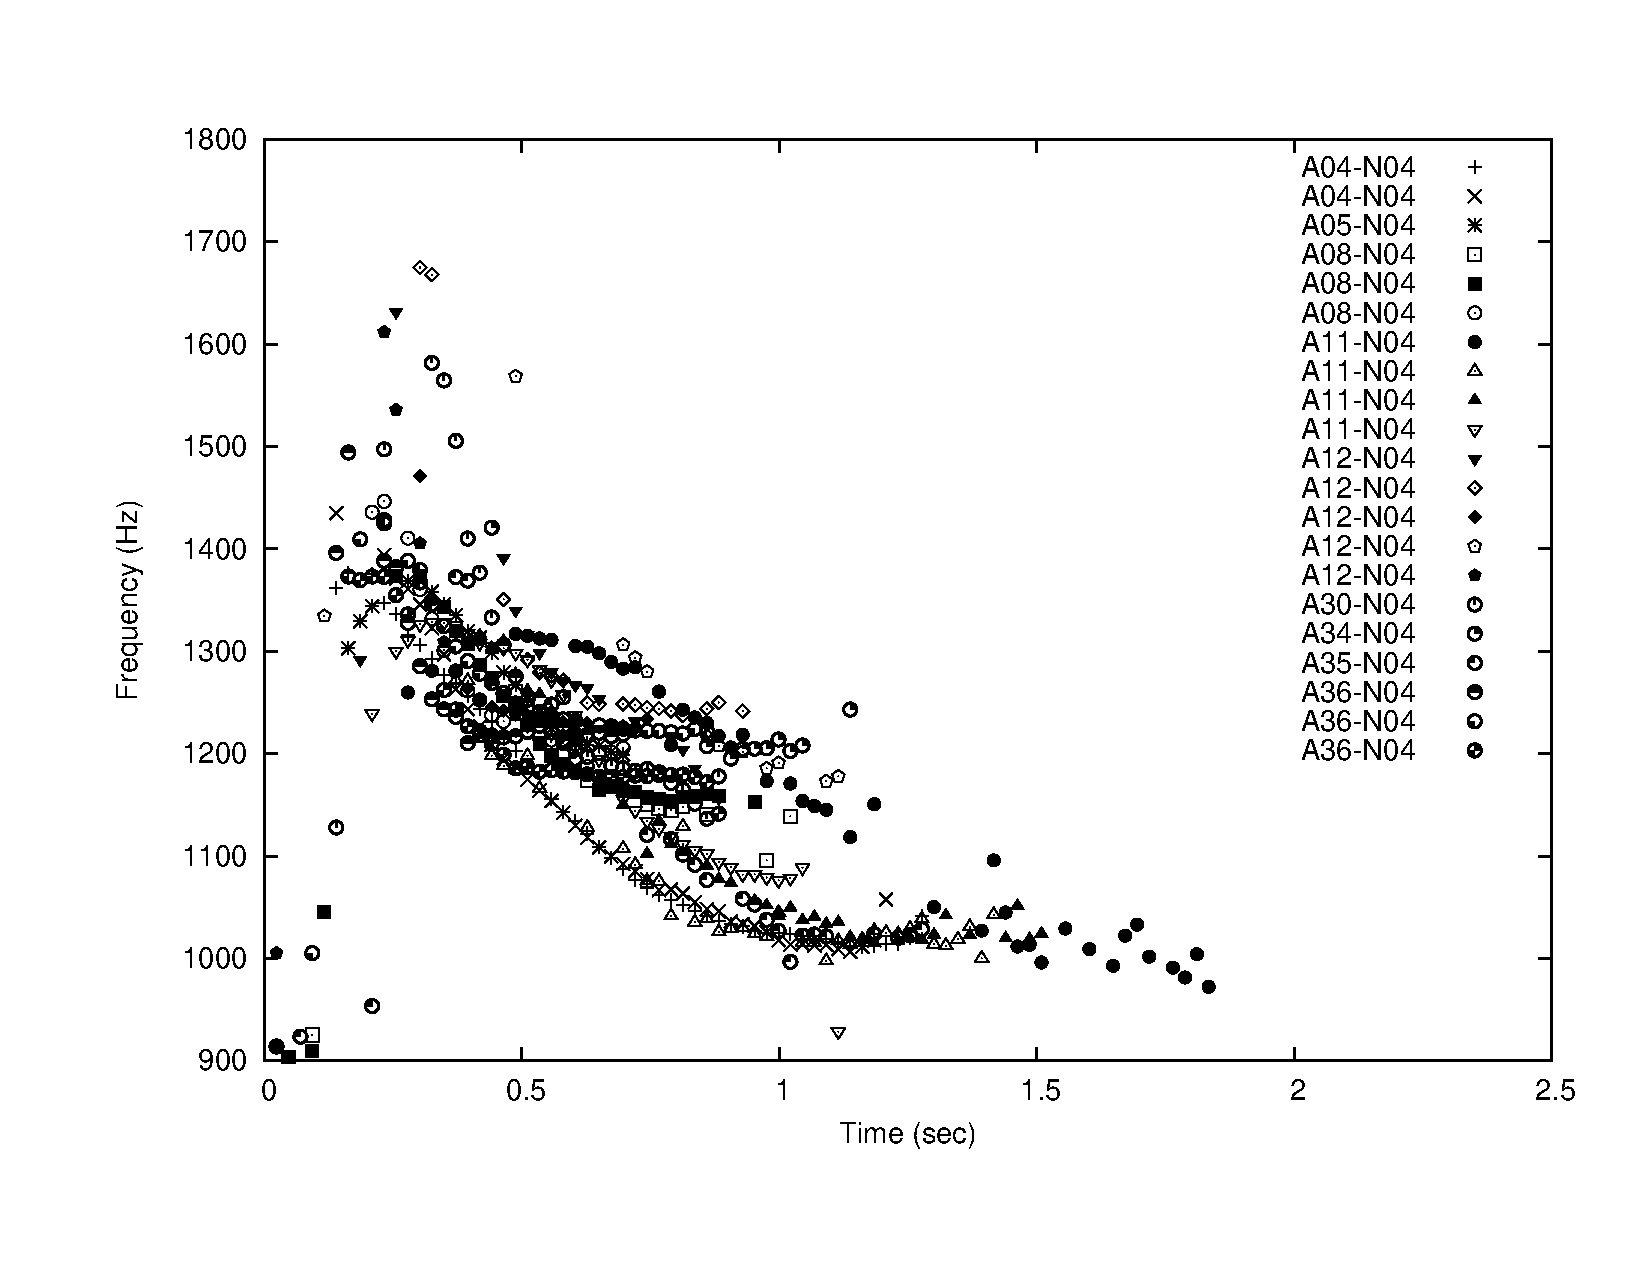
\includegraphics[width=1.0\columnwidth]{figures/pitch-N04}
%% \caption{F0 contour for 21 examples of the N04 call.}
%% \label{fig:pitch-N04}
%% \end{figure}

%% \begin{figure}[h]
%% \centering
%% 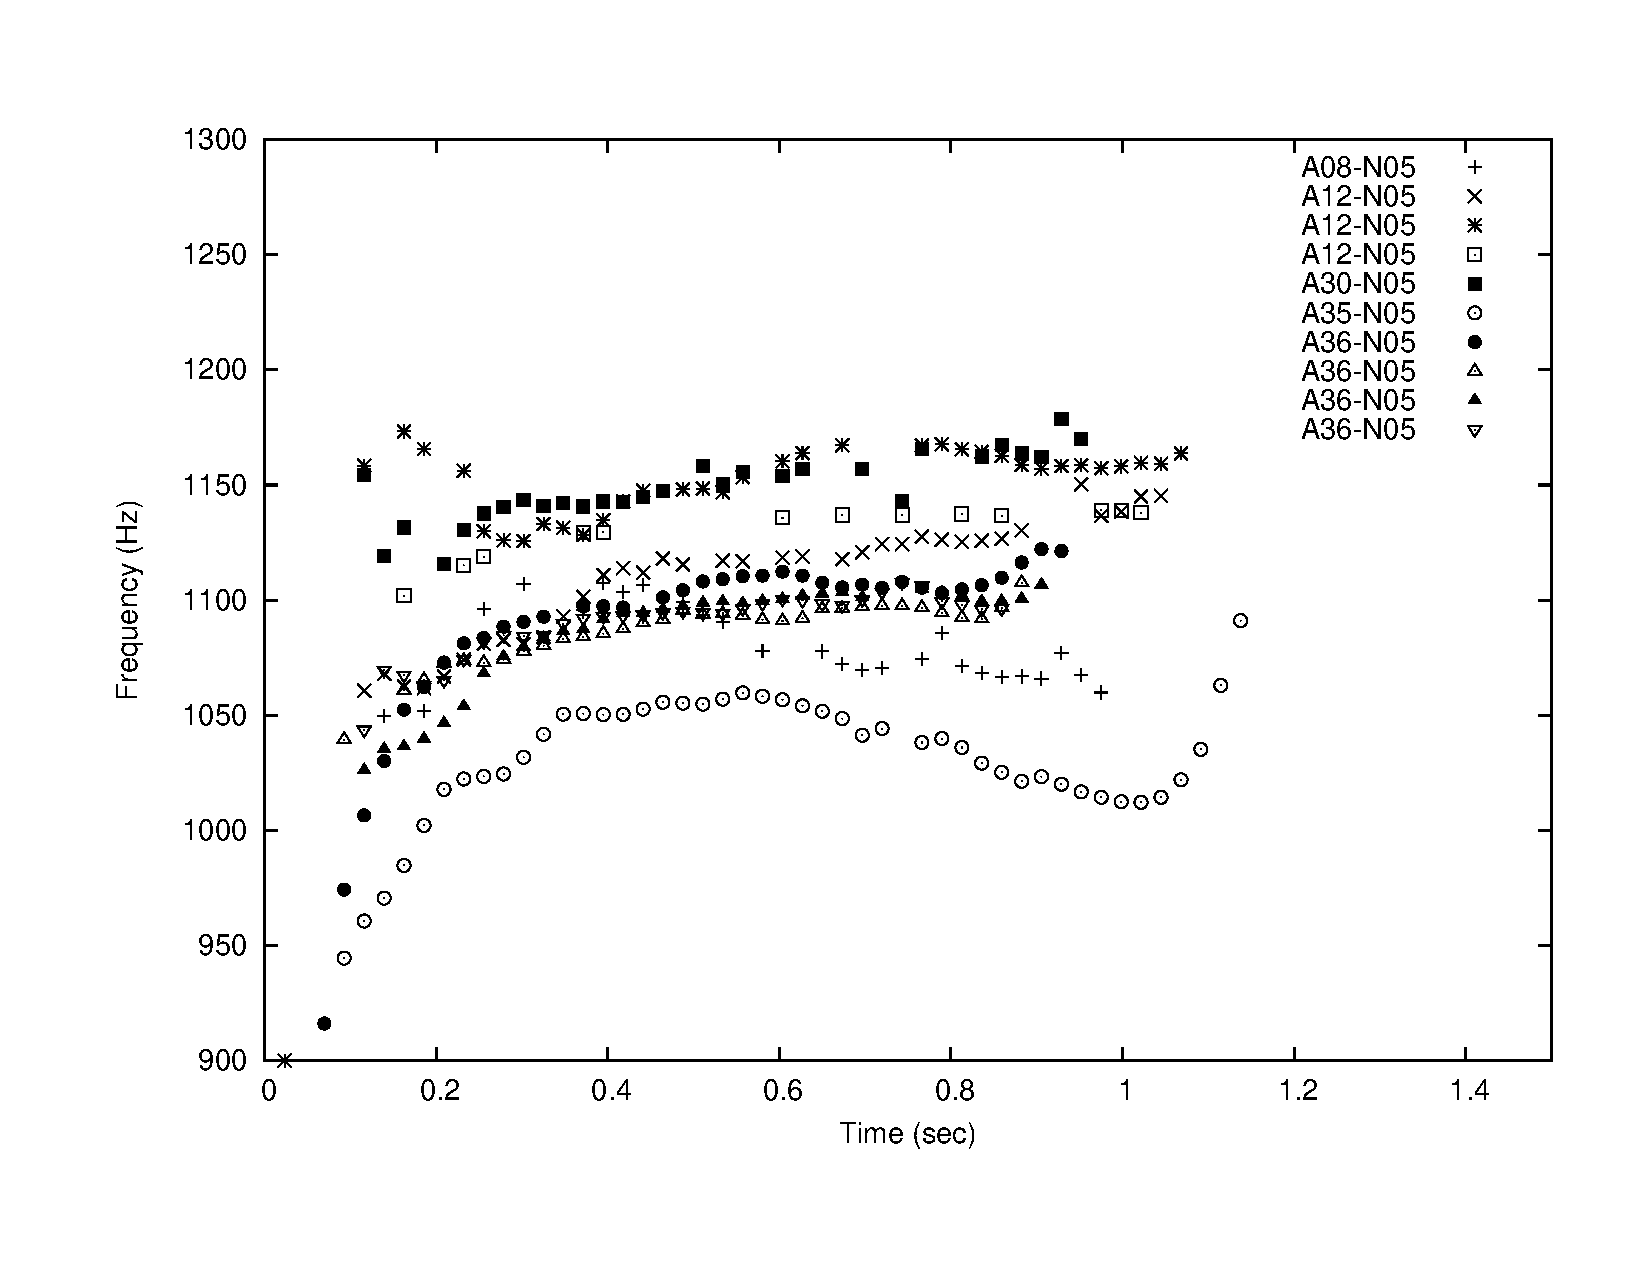
\includegraphics[width=1.0\columnwidth]{figures/pitch-N05}
%% \caption{F0 Contour for 10 examples of N05 call.}
%% \label{fig:pitch-N05}
%% \end{figure}

%% Initialy we tried SAX using the
%% jMotif \footnote{\url{http://code.google.com/p/jmotif/}} Java package
%% but we did not get the results we expected.  For future work, we have
%% begun developing our own Python implementation of SAX to better
%% understand and implement the underlying algorithms.

%% This lead us to develop a different technique which we term
%% Fundamental Frequency Time Series Quantization (FTSQ).  FTSQ is a time
%% series quantization approach that transcribes an audio time series
%% based on an estimate of its fundamental frequency ($F_0$).  In general
%% it is not feasible to analyze Orca vocalizations as a raw time series,
%% since these signals are a complex mixture of sinusoids and noise (see
%% Figure \ref{fig:audio_raw}).  Figure \ref{fig:freqspec} shows a
%% spectrogram representation of the N01 and N09 Orca vocalizations.
%% When comparing Figures \ref{fig:audio_raw} and \ref{fig:freqspec} it
%% is easy to see that the frequency components of the audio signal
%% reveals much more about the structure of the signal than a raw audio
%% time series by itself.

%% \begin{figure}[h]
%% \centering
%% 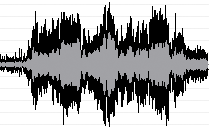
\includegraphics[width=0.4\columnwidth]{figures/audio_raw}
%% \caption{Raw audio signal of Orca vocalization N01.}
%% \label{fig:audio_raw}
%% \end{figure}
%% \begin{figure}[h]
%% \centering
%% 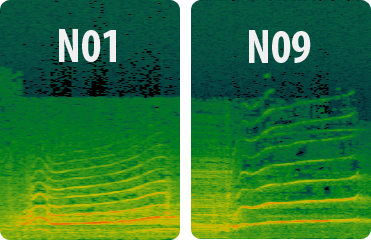
\includegraphics[width=0.60\columnwidth]{figures/freq_N01N09.png}
%% \caption{Frequency spectrum of Orca vocalizations N01 and N09.}
%% \label{fig:freqspec}
%% \end{figure}

%% Quantizing the fundamental frequency of an audio signal is an approach
%% that makes use of the underlying structure in the frequency bands of
%% the audio signal.  Loosely speaking one may think of the fundamental
%% frequency as the pitch of a sound signal.  For our FTSQ technique we
%% use Yin \cite{cheveigne2002yin} a robust fundamental frequency estimation
%% algorithm developed by Cheveigne et al.  Processing the audio waveform
%% from Figure~\ref{fig:audio_raw} with Yin yields the fundamental
%% frequency (in octaves relative to 440 Hz) shown in the top plot of
%% Figure \ref{fig:yin}.  The two plots below the fundamental frequency
%% show the aperiodicity and the period-smoothed instantaneous power of
%% the signal; they give estimate in the confidence on the approximation
%% of $F_0$ and are used to identify meaningful regions of interest
%% within the $F_0$ signal.
%% \begin{figure}[h]
%% \centering
%% 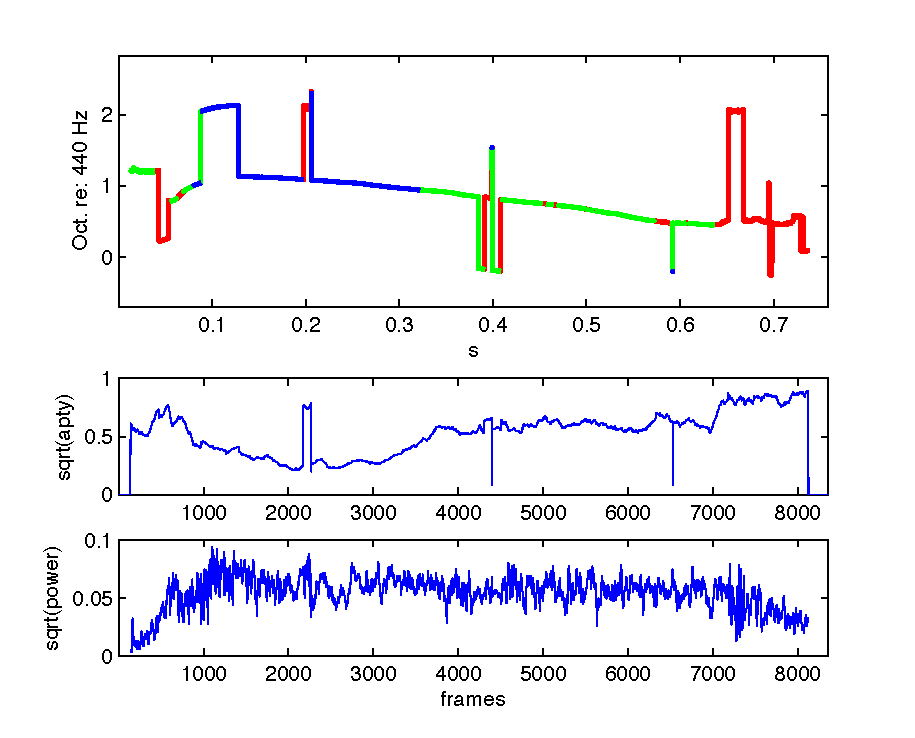
\includegraphics[width=\columnwidth]{figures/yin.pdf}
%% \caption{Frequency spectrum of Orca vocalizations N01 and N09}
%% \label{fig:yin}
%% \end{figure}


%% A further issue that is encountered commonly in the process of
%% determining a pitch contour for an audio recording is the optimization
%% of all the parameters of the pitch detection algorithm to perform well
%% on the particular dataset that is being used.  There are many such
%% parameters for each different algorithm, the important ones in the Yin
%% algorithm include the window size and hop size of the FFT, the high
%% and low frequency cutoffs, the high and low frequencies around which
%% the pitches will be wrapped using modulo arithmetic, the tolerance of
%% the Yin algorithm which determines which peaks in the autocorrelation
%% will be used for the pitch determination, the window size for the
%% median filter, and the number of histogram bins in which to divide the
%% frequency range into.  In our previous work, this was done by hand by
%% plotting points using MATLAB or Gnuplot, which can be a long and
%% labour intensive process.

%% For this project, we added custom visualization tools to our Orchive
%% platform to view the original audio as a spectrogram, to allow the
%% user to listen to this audio, to show a pitch contour with dynamic
%% controls over these various parameters, and an energy display that
%% shows the RMS energy of the audio signal.  This interface is shown in
%% Figure \ref{fig:openmir}.  This software allowed us to quickly iterate
%% over a large number of parameters, and to determine the optimal
%% parameters for the Yin algorithm.  The most important of these was the
%% median filter size, and a median filter of size 11 is shown in Figure
%% \ref{fig:openmir}.

%% \begin{figure}[t]
%% \centering 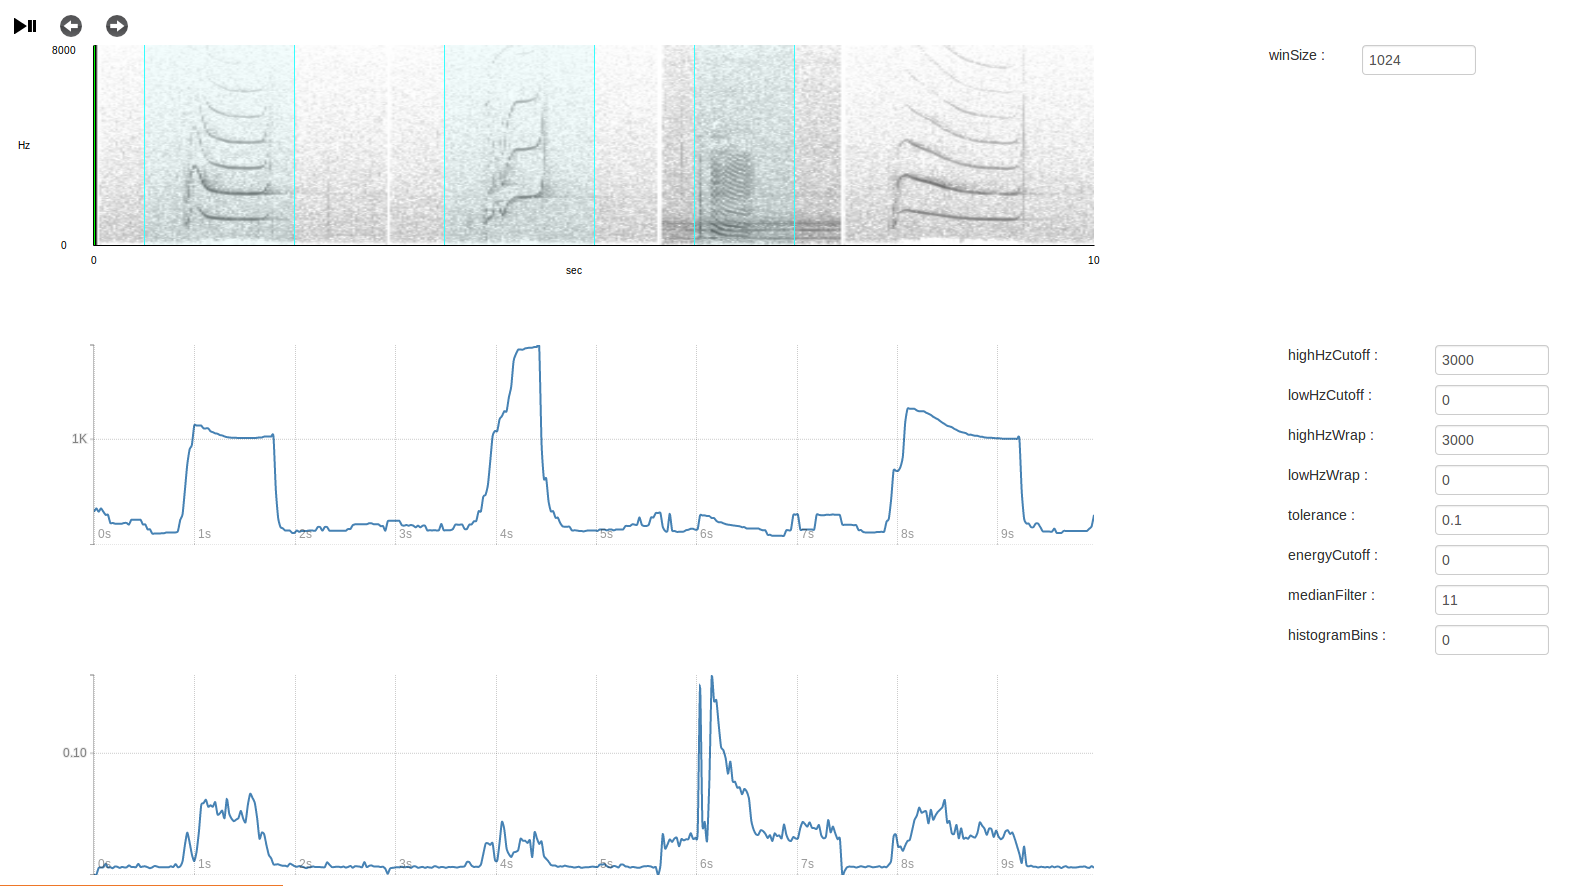
\includegraphics[width=\columnwidth]{figures/openmir}
%% \caption{Spectrogram, pitch and RMS view of a small portion of the Orchive
%% catalog viewed with the OpenMIR interface. }
%% \label{fig:openmir}
%% \end{figure}

%% The output of Yin does not always give a proper estimate of $F_0$.
%% Indeed, the $F_0$ signal in Figure \ref{fig:yin} displays several
%% estimation errors that we herein refer to as \emph{octave errors}.
%% Octave errors manifest themselves as sudden jumps in a multiple of the
%% core $F_0$ frequency. Figure \ref{fig:yin} displays multiple octave
%% errors the first one at about 0.1 seconds. When quantizing the $F_0$
%% signal into a letter representation over a finite alphabet. Octave
%% errors result in mis-mapped letters in the output sequence. To a
%% certain degree we are able to handle octave errors by crafting a
%% custom substitution matrix in our sequence alignment
%% algorithm. However, doing so ultimately lowers the confidence in our
%% alignment score and might confuse legitimate frequency jumps with
%% octave errors and as a result would not penalize mismatches
%% appropriately. Therefore, we have developed a technique that can
%% automatically correct for the majority of octave errors and as a net
%% effect produces a more accurate letter representation.

%% We first run the $F_0$ signal obtained from Yin through a median
%% filter, which smoothes the signal and eliminates small transients that
%% occur due to noise in the original signal. We then threshold the
%% aperiodicity and the period-smoothed instantaneous power to obtain
%% $F_0$ signal regions at which the $F_0$ signal is estimated with high
%% confidence. After down-sampling the signal we obtain the
%% representation shown in Figure \ref{fig:clean_yin}.

%% \begin{figure}[h]
%% \centering
%% 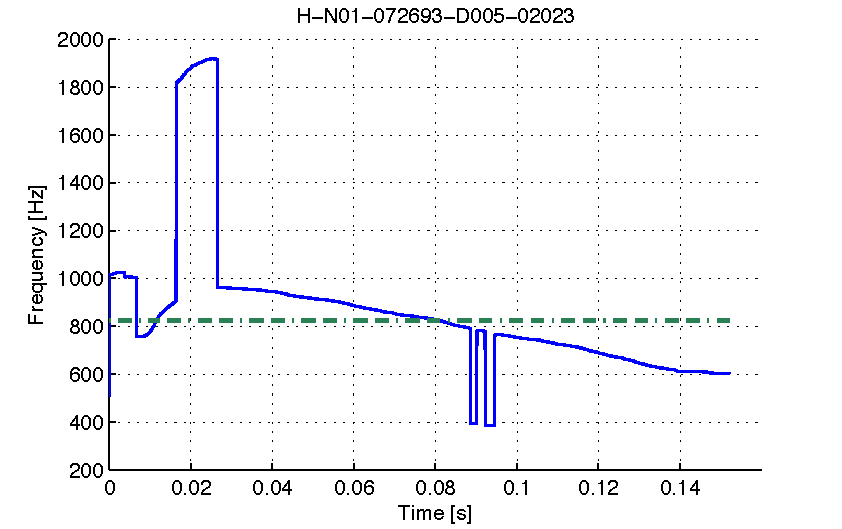
\includegraphics[width=\columnwidth]{figures/yin_clean.pdf}
%% \caption{Thresholded and down-sampled $F_0$ signal of a N01 call.}
%% \label{fig:clean_yin}
%% \end{figure}

%% The green line represents the median of the original $F_0$ signal
%% drawn in blue. The octave errors are clearly identifiable as such in
%% Figure \ref{fig:octave_yin} which shows versions of the $F_0$ signal
%% one octave above (purple) and on octave below (red) the original
%% (blue).  $F_0$ signal. To correct for octave errors we simply piece
%% the portions of the three versions of the $F_0$ signal together
%% according to which ever signal is closest to a slightly upwards biased
%% median of the original signal (blue). This yields the black $F_0$
%% curve wich shows the now automatically corrected version of the $F_0$
%% signal.
%% \begin{figure}[h]
%% \centering
%% 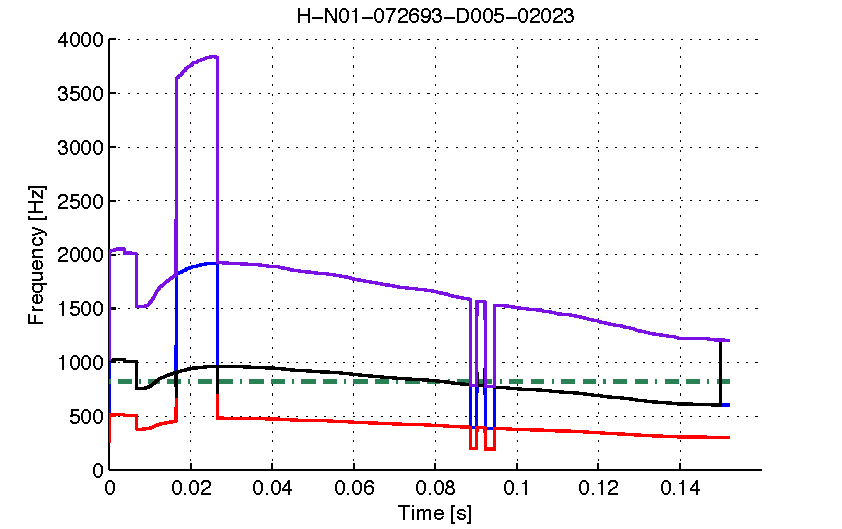
\includegraphics[width=\columnwidth]{figures/octave_fix}
%% \caption{Octave errors within a $F_0$ signal of a N01 call.}
%% \label{fig:octave_yin}
%% \end{figure}

%% When transcribing the $F_0$ signal into a letter representation
%% suitable for sequence alignment tools it is natural to ask how these
%% letters should be assigned over the range of possible $F_0$ frequency
%% values. A naive approach would be to map $F_0$ frequencies to letters
%% in a linear fashion. However, while this approach does work well in
%% practice, we investigated if a non-linear mapping might potentially be
%% more appropriate. For this purpose we plotted the distribution of
%% $F_0$ frequencies over time for the whole catalog of Orca
%% vocalizations in Figure \ref{fig:freq_dist}. The dynamic range of
%% $F_0$ incorporates frequencies from about 80 to 2400Hz, with three
%% high density bands at around 250, 700 and 1200Hz. Ideally one would
%% therefore quantize the $F_0$ signal using a three-modal
%% distribution. However, for simplicity we chose a log-normal
%% distribution (see Figure \ref{fig:log_norm}), which provides us with a
%% fine resolution for the more common $F_0$ frequencies and quantizes
%% high $F_0$ frequencies at a coarser level.
%% \begin{figure}[h]
%% \centering
%% 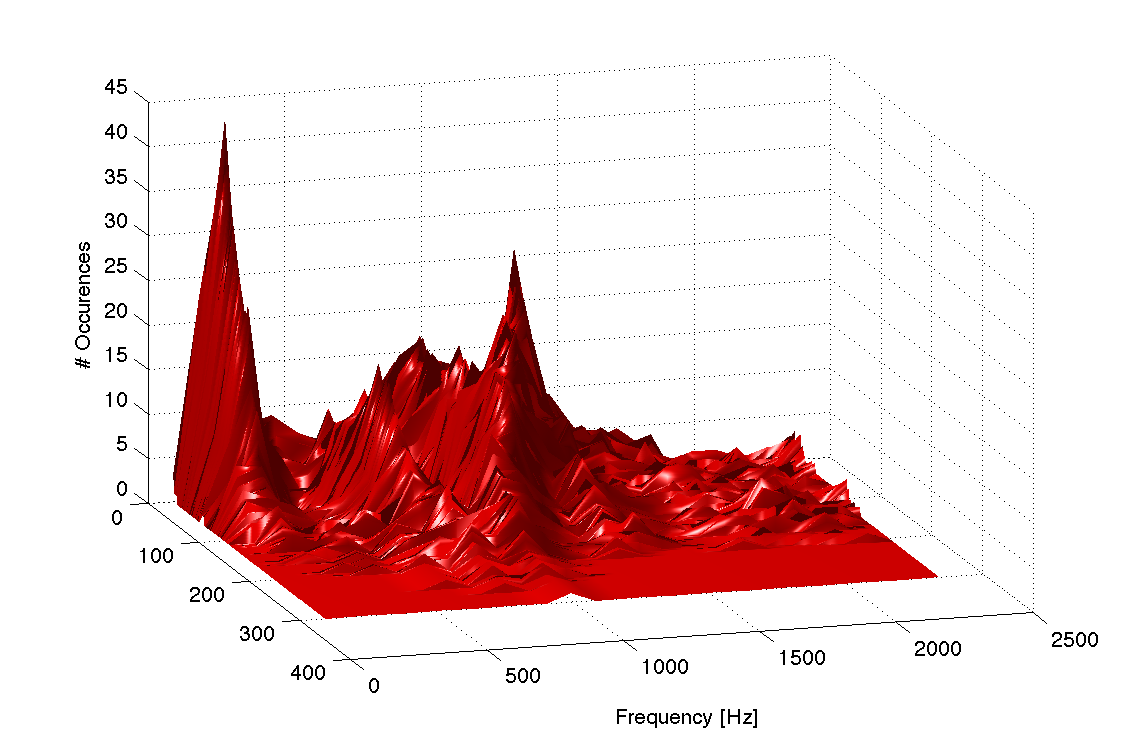
\includegraphics[width=\columnwidth]{figures/freq_dist}
%% \caption{Distribution of $F_0$ frequencies of call catalog.}
%% \label{fig:freq_dist}
%% \end{figure}

%% \begin{figure}[h]
%% \centering
%% 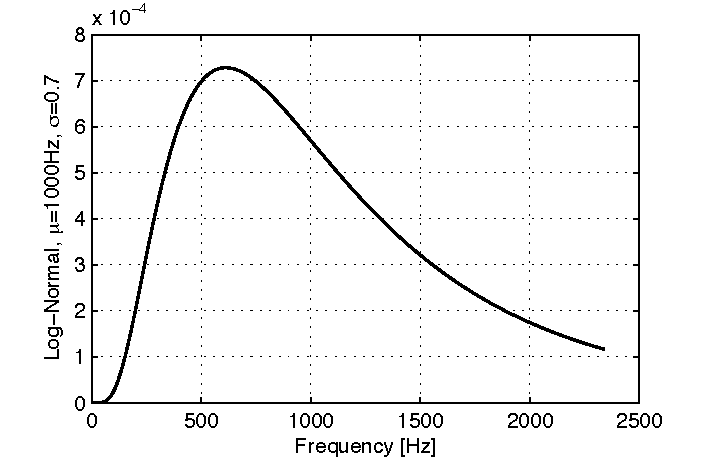
\includegraphics[width=0.7\columnwidth]{figures/log_norm}
%% \caption{Log-normal distribution for quantization}
%% \label{fig:log_norm}
%% \end{figure}

%% The result of log-normal quantization of the $F_0$ trace in Figure
%% \ref{fig:octave_yin} is provided in Figure
%% \ref{fig:letter_curve}. Finally, the resulting letter sequence is
%% given by:

%% \texttt{LLHHJJKKKKKKKKKKKKJJJJJJJII--IIIIIHHHHHHHGGGGGFFFFFF}\\

%% which can readily be consumed by a dynamic programming sequence
%% alignment algorithm.

%% \begin{figure}[h]
%% \centering
%% 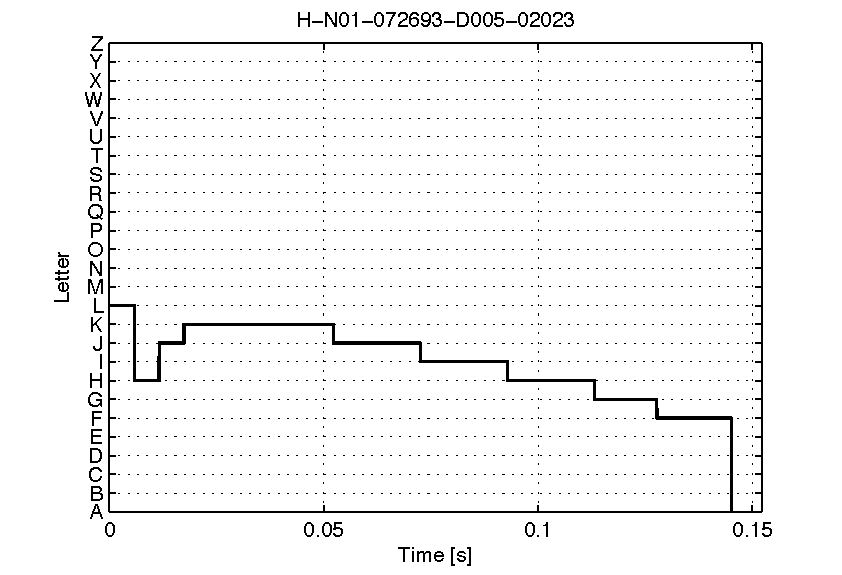
\includegraphics[width=\columnwidth]{figures/letter_curve}
%% \caption{$F_0$ signal of N01 call quantized to a finite alphabet}
%% \label{fig:letter_curve}
%% \end{figure}

%% \begin{table}
%% \centering
%% \begin{tabular}{|c|c|} 
%% \hline
%% Data Set                         &  Global Accuracy  \\
%% \hline
%% Original                         &              64\%  \\
%% Octave Removal - Linear          &              81\%  \\
%% Octave Removal - NonLinear 900   &              80\%  \\
%% Octave Removal - NonLinear 1200  &              81\%  \\
%% J48                              &              58\%  \\
%% Naive Bayes                      &              65\%  \\
%% SVM                              &              75\%  \\
%% \hline
%% \end{tabular}
%% \caption{Global accuracy for different methods of converting a Yin
%%   pitch contour into an alphabet using FTSQ}
%% \label{table:performance}
%% \end{table}

%% \begin{table}
%% \centering
%% \begin{tabular}{|c|c|} 
%% \hline
%%  Call  &  Accuracy  \\
%% \hline
%%  N47   &     0.400  \\
%%  N01   &     0.969  \\
%%  N12   &     0.583  \\
%%  N05   &     0.785  \\
%%  N04   &     1.000  \\
%%  N03   &      0.75  \\
%%  N09   &     0.772  \\
%% \hline
%% \end{tabular}
%% \caption{Global accuracy for different call types using Octave Removal
%%   NonLinear 1200 parameters with the FTSQ algorithm.}
%% \label{table:performance}
%% \end{table}

%% In order for sequence comparison algorithms to work well, it is
%% necessary that the combination of the letters and the scoring matrix
%% are compatible and output meaningful results.  In the two sections
%% below, we show the result of quantizing the signal using the nonlinear
%% histogram approach for two of the more common calls vocalized by
%% A-clan Northern Resident whales.  The first is the very common N4
%% call, which consists of a quick up swing in pitch, followed by a
%% downswing and then a constant tone.  In it we can clearly see long
%% regions of the repeated letters, P,O,N,M,L,K.  Even from a quick
%% visual inspection these repeated letters show that our method of
%% converting frequencies into a discrete alphabet is promising.

%% {\tiny
%% \begin{verbatim}
%% N04 A04 HIKNOOOOOPPPPOOOOOOOOOOOONNNNNNNNNNNNMMMMMMMMMMMMLLLLLLLLLLLLLLLLLLKKKKKKKKKKKKKKK
%% N04 A04 IJNOPPPPPPPPPPPOOOOOOOOONNNNNNNNMMMMMMMMMMMMMMLLLLLLLLLLLLLLLLLLLLLLKKKKKKKKKKKKKK
%% N04 A05 NLKLMNOOOOOOOOOOOOOOOOOOOOOOOOOONNNNNNNNNNNNNNNNNNNNMHGQ
%% N04 A08 RILMNNOOOOOOOOIIOOOOOOOOOOONNNNNNNNNNNNNNNNNNNNNMMMMMMMMMMMMMMMMMMMMMLLLLLLLMLLLLL
%% N04 A08 SIIJJKNPQQRPIIOOOOOOOONNNNNNNNNNNNNNMMMMMMMMMMMMMMMMMMMMMMMMMMDCCCMMM
%% \end{verbatim}
%% }

%% Even more promising were the results for another call, N5, which
%% consists of a constant tone.  These calls are from the A36 matriline
%% of orcas, which now consists of only two whales, the brothers A37 and
%% A46, although the grandmother whale, A12 often now associates with
%% this matriline after A34, her daughter's matriline, grew large in
%% size.  From these calls, we can see that the frequency represented by
%% the letter L is very constant throughout the entire call, and is a
%% clear indication that this is an N5 call.

%% {\tiny
%% \begin{verbatim}
%% N05,A36,A36-N05-070806-D012-13913,IIJJJKKKKKLLLLLLLLLLLLLLLLLLLLLLLLLLLLLLLLLLLLLLLLLLLLLL
%% N05,A36,A36-N05-070806-D012-13917,JJJKKLLFLLLLLLLLLLLLLLLLLLLLLLLLLLLLLLLLLLLLLLLLLLLLLLLL
%% N05,A36,A36-N05-070806-D012-13921,IIJJKKKKKKKKKLLLLLLLLLLLLGLLLLLLLLLLLLLLLLLLLLLLLLLLLLLL
%% N05,A36,A36-N05-071506-D017-11311,IQHJKLLLLLLLLLLLLLLLLLLLLLLLLLLLLLLLLLLLLLLLLLLLLLLLLLLL
%% \end{verbatim}
%% }

%% Most of the existing work in the automatic analysis of Orca calls has
%% focused on detection and classification rather than retrieval. A
%% real-time system with low computational requirements for the detection
%% of Orca vocalizations is described in
%% \cite{luke2010realtime}. Annotation bootstrapping is a technique used
%% to classify/segment hydrophone recordings into three broad categories:
%% voiceover, background, and vocalizations \cite{ness2008chants}.



%% Work done using a system similar to Symbolic Aggregate Approximation
%% (SAX) to transform pitch contours into a string representation, which
%% would allow the use of algorithms from bioinformatics to efficiently
%% search the entire Orchive for repeated patterns.  The highest
%% classfication accuracy for calls obtained with this system was 81\%,
%% which shows the potential utility of this algorithm for finding calls
%% and other repeated patterns in the audio from the Orchive.  This high
%% classification accuracy shows the success of this part of the system
%% described in this thesis.




%% \section{System Overview}
%% \label{section:softwareAndSystems:systemOverview}

%% Given the vastness of this archive, there are certainly many different
%% tasks that bioacousticians and other scientists might want to use it
%% for, but one primary obstacle is that the recordings in the Orchive
%% are currently mostly unlabeled.  After \totalYearsAnnotationsCollected
%% years, there are \totalAnnotations annotations in the Orchive, which
%% represents only a few hours of actual annotated time.  Even with many
%% scientists working on labeling this data, it would take many
%% person-years to label the entire Orchive.  By using a combination of
%% expert users and machine learning software, it is possible to train
%% machine learning classifiers on expert labeled data and from there to
%% predict the location of orca vocalizations.  


%% With these interfaces, we are able to label substantial amounts of
%% data but are still far away from labeling the entire
%% \totalNumberOfOrchiveRecordings hour archive.  In order to do this,
%% researchers have commonly used a combination of the techniques of
%% audio feature extraction and machine learning to classify audio.  In
%% this thesis, we will use a combination of audio feature extraction and
%% machine learning to identify sections of the Orchive where there are
%% clear orca pulsed vocalizations that are distinct and not overlapping
%% with the vocalizations of other orcas and are relatively free of boat
%% noise. These extracted vocalizations will then be made available to
%% the scientific community and will also be used by our lab in future
%% work for answering other scientific questions about this species.

%% In order to do this, we will compare a number of different solutions
%% for doing distributed audio feature extraction and machine learning
%% and will compare not only their performance in classifying audio but
%% also our experience with using these tools.

%% For the evaluation, we will generate two different types of results.
%% The first type will be the output of the audio feature extraction and
%% machine learning task. For this task, we will look at the distribution
%% of orca vocalizations in the dataset, and will train machine learning
%% classifiers that can distinguish regions of the Orchive that have
%% individual orca vocalizations.

%% In order to analyze the audio in large online archives efficiently, a
%% scenario involving distributed computing must be used.  There are many
%% different types of systems that perform machine learning and many of
%% these can distribute their work to different machines.  Some of these
%% systems are better suited for this task than others, and in this thesis,
%% we investigate a few combinations of these tools.

%% One of the possible solutions to the problem of the segmentation of
%% audio into orca vocalizations and other sounds is to use a Machine
%% Learning supervised classifier system.  These systems require hand
%% labeled training data; in our particular case, audio would be labeled
%% as either orca or background.  This training data is then used to
%% train a classifier system that can classify future instances based on
%% features of the training data.  There are a wide variety of
%% classification algorithms that are commonly used, some of the most
%% popular are Support Vector Machines (SVMs)\cite{cortes1995svm}, Neural
%% Nets \cite{hinton2006fast}, Decision Trees \cite{quinlan1993c45} and
%% Logistic Regression \cite{lecessie1992logisitic}.  In our past work
%% \cite{ness2008chants}, we have found good success in using SVMs, and
%% have shown that SVMs typically outperform many other machine learning
%% algorithms.  However, there is current work in this area showing the
%% benefits of many alternate algorithms for different problem domains.

%% There are two steps to the problem of the classification of audio
%% signals.  The first is that of audio feature extraction, and the
%% second is that of classification with machine learning systems.  Sound
%% is a pressure wave in the air, and the variations in pressure over
%% time can be stored in a computer as real number values.  This raw
%% waveform data contains all the information of the signal but because
%% of its extremely high dimensionality is difficult to analyze with
%% machine learning systems.  To take this raw data and to put it in a
%% form more conducive for analysis, we generate a large number of higher
%% level features, including spectral features
%% \cite{tzanetakis2008marsyas}, pitch information
%% \cite{cheveigne2002yin}, chromatic scale information
%% \cite{tzanetakis2008marsyas}.  One can also model the statistical
%% behaviour of these properties as they change over time; an avenue that
%% has been shown to be fruitful \cite{tzanetakis2008marsyas}.  In our
%% system, we investigated the use of a number of audio features, the
%% results of which are discussed in Chapter \ref{chap:evaluation}.

%% The second step is to take these audio features, train and test a
%% machine learning classifier on them, and then run this Machine
%% Learning classifier over all the data.  In some cases, if disk space
%% permits, it is beneficial to pre-calculate the audio features for the
%% data.  Once good parameters can be determined for the audio feature
%% extraction engine, such as the window size, hop size for the spectrum
%% calculation and the memory size for the texture window statistical
%% calculations, these features can be saved and reused in multiple
%% machine learning experiments with different parameters.  One example
%% of this is the recent release of the Echonest audio features for the
%% Million Song Dataset \cite{bertinmahieux2011million}.  This collection
%% of audio features for one million popular songs took a considerable
%% amount of time to process, and one approach commonly used in the
%% machine learning community is to save these audio features and run
%% different machine learning algorithms and different sets of parameters
%% for these algorithms on them.  Another point that should be made here
%% is that the form of the features that are extracted in this step can
%% have a direct relation to the performance of the subsequent Machine
%% Learning step.  Matching appropriate audio features with suitable
%% algorithms often requires an extensive search process and is
%% facilitated by experience on the part of the individual researcher.

%% It should be noted that both of these steps, the audio feature
%% extraction and the machine learning, could be carried out in the same
%% executable.  There are a number of advantages to this as well as some
%% disadvantages.  One major advantage is that the intermediate audio
%% feature data does not have to be saved on disk.  This intermediate
%% data can be very large in size and can be many times larger in size
%% than the original audio data depending on the type of compression
%% used for the original audio.  In many cases in the real world, it is
%% less expensive to just recalculate the audio features each time that a
%% new machine learning run is carried out rather than saving them on
%% disk.  This also can help to overcome any versioning problems, where
%% different versions of audio features are combined together in the
%% training, testing or predicting stages.  It will be a balance between
%% these two poles for production systems to manage.

%% For this work, Marsyas was used for doing audio feature extraction.
%% There are other Music Information Retrieval toolkits for extracting
%% audio features, but the audio features output by Marsyas are typically
%% amongst the most robust and high performing in the literature
%% \cite{tzanetakis2008marsyas}.  We have implemented this feature
%% extraction using native filesystem operations loading data off of NFS
%% or a local disk depending on the cluster setup.

%% The primary task that will be investigated in this project will be the
%% identification of regions of the Orchive with distinct orca
%% vocalizations that are nearby to hydrophones and isolated from other
%% orca vocalizations and to assign them classes based on the Ford
%% \cite{ford1989acoustic} call catalog.  The software system described
%% in this chapter is instrumental in both the collection of the data to
%% train the machine learning classifiers and to validate the
%% classifications using citizen scientists and experts.  By the end of
%% this thesis, one version of the ORCACALL and ORCAOBV datasets will be
%% created and evaluated, but it will be an ongoing community project to
%% correctly label all of the audio in the Orchive.

%% There are a number of large bioacoustic archives that have been
%% described in the literature, and as computer storage grows ever
%% larger, more of these archives are being created.  In this work, we
%% describe a large bioacoustic dataset, the Orchive, which is an archive
%% of sounds collected by a network of stationary, permanently mounted
%% hydrophones, and the primary sound that was of interest to the
%% researchers was that of Orcas.

%% The majority of the audio recordings consist of three broad classes of
%% audio signals: background noise caused mainly by the hydrophones,
%% boats, background noise containing orca vocalizations and voice over
%% sections where the observer that started the recording is talking
%% about the details of the particular recording. In some cases there is
%% also significant overlap between multiple orca vocalizations. The orca
%% vocalizations frequently can be categorized into discrete calls
%% \cite{ford1991vocal} that allow expert researchers to identify their
%% social group (matriline and pod) and in some cases even allow
%% identification of individuals.

%% Even when the data is digitized, locating a particular segment of
%% interest in a long monolithic audio recording can be very tedious as
%% users have to listen to many irrelevant sections until they can locate
%% what they are looking for. Even though visualizations such as
%% spectrograms can provide some assistance, this is still a task that
%% requires much manual effort. In this thesis, we describe experiments for
%% the automatic classification and segmentation of the orca recordings
%% for the purposes of locating segments of interest and facilitating
%% interaction with this large audio archive.

%% The main task in this work is to develop machine learning systems to
%% first segment recordings into the classes orca/background/voice.
%% These systems should discriminate between the many kinds of background
%% noise that can be found on the recordings, all different orca calls
%% and voice notes.  Once we have identified clips containing orca
%% vocalizations, the second task is to classify these calls based on a
%% previously existing call catalog, in this case the one developed by
%% John Ford \cite{ford1989acoustic}.

%% Over the past \totalYearsAnnotationsCollected years, a number of orca
%% researchers using our website have added \totalAnnotations clip
%% annotations to our database.  A small section of annotated audio from
%% the Orchive is shown in Figure \ref{fig:dm_orchive}.  These clip
%% annotation are of two main types: The first is clips that
%% differentiate background noise from orca calls and from the voice
%% notes of the researchers that collected the data.  The second type of
%% clip annotations classify orca vocalizations into different calls.

%% \section{Machine Learning}
%% \label{section:softwareAndSystems:machineLearning}

%% In addition to the presentation and collaborative annotation that the
%% Orchive supports, we have also developed a set of Music Information
%% Retrieval and machine learning tools that are available for
%% researchers to run on the data in the Orchive. All of these tools are
%% part of the Marsyas \cite{tzanetakis2008marsyas} MIR framework.

%% There exist a large number of algorithms in the field of Music
%% Information Retrieval (MIR)\cite{futrelle2002mir} that could be
%% successfully used for the study of orca vocalizations.  Some of these
%% include the FFT and Power Spectrum, measures of the shape of this
%% spectrum including Centroid, Flux and Rolloff and statistics of the
%% change in these quantities over time.

%% One important design goal in this project is to make our system as
%% flexible and extensible as possible.  To this end, we have come up
%% with a keyword-based system that allows researchers to construct their own
%% ontologies.  Some of these ontologies would overlap, like ``orca'' or
%% ``voiceover'', and some would be distinct to different areas of study.
%% By allowing a user defined structure to emerge, we empower individual
%% research communities to ask and answer the questions most pertinent to
%% them.  The obvious drawback to this is that within communities
%% researchers must agree on the same language and syntax to annotate
%% calls.  We hope to provide tools within and external to the site to
%% help encourage the collaboration necessary to converge on the same
%% vocabulary.

%% \section{System Overview}
%% The system developed in this paper includes a web-based interface to
%% allow researchers to listen to, view and annotate this audio, tools to
%% extract and view audio features from this data, and tools to run
%% machine learning software and view the results of this analysis.

%% In order to further add to the training data for the machine learning
%% classifiers, we have also built simple iPad and web-based casual games
%% with a serious intent, which we call serious casual games.  Casual
%% games are those like the well known Solitaire, which take a short
%% amount of time to play and do not require all the users attention.  By
%% allowing these citizen scientists to assist us, we are able to collect
%% larger amounts of data and to sort through data we have generated
%% quickly.  In fact, one of the main users of this game software has
%% been ourselves; we find the game interface a quick and effective way
%% to label training data.

